%!TEX root = ../thesis.tex

\chapter{Challenges in ASR and Role of AI in \\ Speech Technology}    % (fold)
\label{cha:why_asr_difficult}

There are more than 6,000 languages globally out of which, only in Europe, 24 are official languages, 5 semi-official languages, and more than 100 additional regional or minority languages with more than 50 million language speakers in Europe if we rank the top 50 languages. Currently, 3,000 different languages are considered to be endangered. The figure \ref{fig:lang-vocab-1} and \ref{fig:lang-vocab-2} show the number of unique and new words in various languages \cite{creutz_morph-based_2007}. Each Language requires a separate language model for Speech Recognition which in turn requires big data. Hence ASR for Low-Resource Language is a serious challenge in this field \cite{besacier_automatic_2014}. 

\begin{figure}[h]
    \centering
    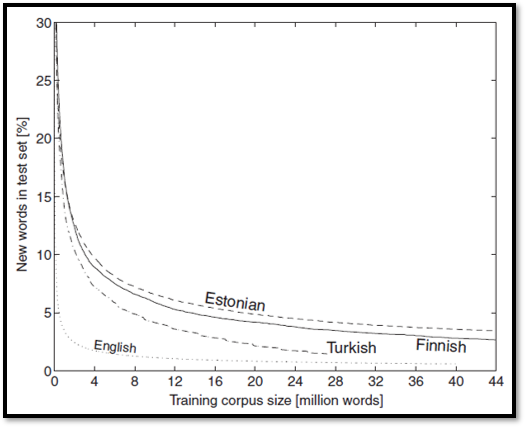
\includegraphics[width=0.5\textwidth]{img/Creutz.png}
    \caption{Languages and Vocabulary (New words) \cite{creutz_morph-based_2007}}
    \label{fig:lang-vocab-1}
\end{figure}

\begin{figure}[h]
    \centering
    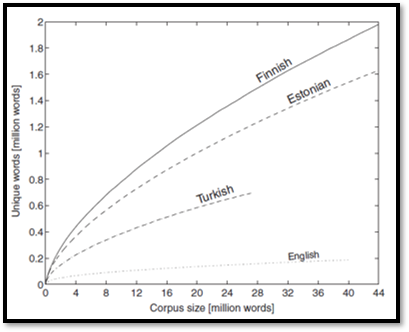
\includegraphics[width=0.5\textwidth]{img/Creutz2.png}
    \caption{Languages and Vocabulary (Unique words) \cite{creutz_morph-based_2007}}
    \label{fig:lang-vocab-2}
\end{figure}

Although ASR research has progressed significantly, but has not reached perfection. Speech recognizers are not very robust and make mistakes for a variety of reasons. We will delve deeper into each type of problem in the ensuing subsections.

\section{Speaker Variation Problems}
\label{sub:speaker_variation}
There are factors with regard to type of speaker which affect the audio information. Following must be catered with regards to Speaker Variation which affects Acoustic Modelling:
\begin{itemize}
    \item \textit{Vocal range} e.g. fundamental frequency, and pitch range \cite{vipperla_ageing_2010}. 
    \item \textit{Speed and length of speech} e.g. This must be planned when training data-set i.e. whether we want to train on isolated or continuous speech \cite{markus_forsberg_why_2003}. 
    \item \textit{Quality of Voice} like whisper, grunt, growl, physiological elements e.g. nasality, adenoidality, etc \cite{shrawankar_adverse_2013}. 
    \item \textit{Accent and dialects}, e.g.vowel systems, consonants, allophones, etc.) which may make it difficult of ASR to recognize words \cite{shrawankar_adverse_2013}. 
    \item \textit{Health, emotional state} etc which can be problematic in speaker verification systems \cite{backstrom_introduction_2022}.
    \item \textit{Speech style} - It is more difficult to build a speech recognizer that recognises only formally read speech than the one that allows the user to speak spontaneously because spontaneous speech is characterised by incomplete sentences, false starts, extended words, poor pronunciation quality, and an infinite vocabulary. \textit{Disfluencies} in spontaneous speech like long pauses, fillers, false starts, hesitations, ungrammatical constructions, and mispronunciations are the primary cause of the difference in recognition error rates between spontaneous and read-out speech. Hence, acoustically and grammatically it is difficult to recognise spontaneous speech \cite{shrawankar_adverse_2013}.
    \item \textit{Prosody} – Stress, intonation, and rhythm convey critical information for word recognition and the user's understanding. These stresses can cause the words to change e.g. in Arabic, the "shad" notation means more stress \cite{shrawankar_adverse_2013, markus_forsberg_why_2003}. So the word Becca with stress on "cc" part will sound different. ASRs face issues recognizing these differences.
    \item \textit{Type of Utterance} -  Every word recognised by a speech recognizer may be recognised independently. It might ask the user to speak each word of the sentence with a fake pause in between, or let them speak normally. There are two different systems in this way:
    \begin{itemize}
        \item \textit{Isolated word recognition system} is the most fundamental recognition strategy which is possible to develop without an LM by using word-based acoustic models. Sentences made up of isolated words become more difficult to recognize as the vocabulary grows, necessitating the usage of sub-word based language and acoustic models \cite{backstrom_introduction_2022}.
        \item \textit{Continuous speech recognition systems} enables users to express themselves in a comparatively or fully unrestricted manner. These recognizers, in presence of all co-articulatory effects, must give a good performance. As a result, development of Continuous Speech Recognition is arduous because word boundaries are ambiguous, and co-articulatory effects are much stronger in continuous speech \cite{markus_forsberg_why_2003}.
    \end{itemize}
   
\end{itemize}

\section{Linguistic Issues}
\label{sub:linguistic-issues-asr}
Linguistic issues make ASR difficult as in this domain following must be catered for:

\begin{itemize}
    \item \textit{Out-of-vocabulary (OOVs)} - Jargon, slang etc are OOVs which are are hard problems of ASRs. 
    \begin{itemize}
        \item The most advanced ASRs on the market today have limited vocabularies and cannot recognise words outside of their training vocabulary.
        \item  For HMM-GMM and neural ASR systems, special techniques for handling OOV words are available for deployment. \cite{zhang_strategies_2019}.
    \end{itemize}       
    \item \textit{Homophone Substitution} - Generally, a well-functioning language model should be able to distinguish homophones based on context. Homo-phonic substitution errors can occur where multiple lexical entries with the same pronunciation or phone sequence called homophones exist. During decoding, homophones cause confusion with one another, resulting in errors, such as the distinction of disambiguation homophones such as "their" and "there" or "hear", "here", "hare" and "hair" \cite{vasilescu_cross-lingual_2011}. %Homophonic substitution in an input utterance confuses the system with a similar word or homophones in its own vocabulary leading to misunderstandings. 
    \item Recognition of \textit{children’s speech} and of \textit{people with speaking disorders} is sub-optimal with standard corpus or any regular kind of training data \cite{kumar_leveraging_2020}.
    \item \textit{Consideration for linguistic structure} i.e. phonetics, morphology, graphemes, etc \cite{creutz_morph-based_2007, backstrom_introduction_2022}. 
    \begin{itemize}
        \item Many languages have a greater morphological richness than English, which has an impact on vocabulary construction and language modelling.
        \item Compounding is used in languages such as German in which compound words are decomposed into constituent parts and then pronunciation and language modelling are performed on the decomposed parts.
        \item All morphology-based approaches aim to reduce ASR errors by reducing the OOV rate through modelling at the morph level, while also accounting for the lack of broad-vocabulary data, as we are not always able to arrange an audio data-set for every word in the dictionary. 
        \item Morphs are used instead of words in morph-based language modelling, but the context may need to be extended because multiple morphs are related to a single word \cite{creutz_morph-based_2007}.
    \end{itemize}  
    \item \textit{Code-Switching} - Often in many areas, no one speaks the particular language purely which is why we need a mix of out-of-language words in the lexicon from other languages \cite{farooq_enhancing_2020}. E.g. in Pakistan, Urdu may be the official language but no one speaks pure Urdu. It is often mixed with some words from English, Panjabi, Hindi, Sindhi and Pashto. This is an issue which we will discuss further in Section \ref{sub:code-switching-problem}. 
\end{itemize}

\subsection{Code-Switching Problem}
\label{sub:code-switching-problem}

Code-Switching is spontaneous use of more than two languages in a single sentence or the whole conversation. It a linguistic phenomenon prevalent in multi-cultural societies as well as in the countries where official language and native language are different e.g. in Pakistan its English and Urdu and in case of Algeria and Tunisia it is French and Arabic etc. It is also an active research area in ASR \cite{farooq_enhancing_2020}.

The following sentence is an example of what types of calls we get in CPLC call center which can be referred to as Urban or code-switched Urdu: 
\begin{quote}
\textit{"Assalamualaikum mujhe urgently aik report darj karani he"}    
\end{quote}

The sentence can be translated in English as \textit{"Peace be on You. I want to urgently file a report."}
\vspace{11pt}
\par
Let us observe the original sentence that has multiple code switches. The first word \textit{"Assalamualaikum"} is a common Muslim greeting that is basically an Arabic word. The next word \textit{mujhe} is an Urdu word followed by an English word, Then urdu, then English and last three words again are Urdu words. For transcription  we kept Roman script instead of Nastaliq for Urdu and Roman for English so that we do not have to do separate language modeling for every language word that occurs in the corpus.

\section{Model Training and Deployment Challenges}
\label{sub:model-training_asr_difficult}

Every language needs a different language model. There are approximately 7,000 languages in the world, the majority of which have limited training resources, code-switching issues, and language change issues, and we cannot create a one-size-fits-all model for them. That requires us to train model for each language as per the scenario \cite{pironkov_hybrid-task_2020}.

Some more factors we need to cater are:
\begin{itemize}
    \item \textit{Robustness} i.e. ability to work despite small errors, having graceful degradation and not catastrophic failure \cite{shrawankar_adverse_2013}.
    \item \textit{Portability} i.e. ease of deployment, independence of computing platform etc \cite{kincaid_state_2018}.
    \item \textit{Adaptability} to changing conditions e.g.  telephonic environment, gender, different speaker, mic, noisy conditions, or even new language etc \cite{kincaid_state_2018}.
    \item \textit{Confidence} Measures i.e. methods to evaluate correctness of hypothesis \cite{backstrom_introduction_2022}.
    \item \textit{Computational} power requirement like GPU, Processors, Electricity availability \cite{kincaid_state_2018}.
    \item \textit{Financial Costs} including hardware, software and HR. Apart from the scale of data, we also need to consider the cost of building applications which are mostly fixed, and don’t scale with the size of our profit. The scale at which we can break even will tend to decrease over time, as the algorithms get better, and the software becomes easier to use but the cost of the training data will still be less than what is paid to ASR engineers \cite{kincaid_state_2018}.
    \item \textit{Availability of Skills} which includes data-scientists and AI Engineers for Speech Processing \cite{kincaid_state_2018}.
    \item \textit{Speaker-independent or Speaker Tuned for a particular speaker} e.g. in case of speaker dependent system, adaptation to speaker characteristics is key \cite{shrawankar_adverse_2013}.
    \item \textit{Hierarchical and Compositional nature of speech production and comprehension} makes it difficult to handle with single model. The decoder may be forced to reject the true hypothesis in favour of a spurious candidate with high language model probability due to an undue Language model bias caused by a high relative weight on the language model. These errors could occur in tandem with analogous acoustic model bias \cite{backstrom_introduction_2022}.     
    \item \textit{Spectral Bandwidth} i.e. with decrease in bandwidth, the performance of the trained ASR system will also decrease, and vice versa.
    \item \textit{Variable Environmental noises} reduce accuracy of ASR \cite{misra_spectral_2004}.
    \item \textit{Overlapping speech} is still a hard problem for ASR system in production environment \cite{chen_progressive_2018}.
    \item \textit{Type Of ASR Approach} to be taken is an important consideration \cite{georgescu_performance_2021}. On lesser data Deep Learning is not as effective as traditional but on larger data-set, we find Deep Learning to improve the accuracy indefinitely (See figure \ref{fig:comparison-all-asr-approach}). 
    \item ASR as a \textit{classification problem} has very high dimensional output space \cite{jurafsky_speech_2009}. 
    \item ASR as a \textit{sequence-to-sequence problem}, has a very long input sequence although limited reordering between acoustic and word sequences \cite{jurafsky_speech_2009}.
\end{itemize}

\section{Data-set Challenges}
\label{sub:data-set-asr_difficult}

\begin{itemize}
    \item \textit{Availability of Data-set} - This is one of the biggest issue for ASR researchers especially in case of low-resource languages. Data available on internet e.g. on Kaggle, GitHub, YouTube etc wouldnot work in every scenario. Sometimes we need Code-switched dataset which adds to problem of availability of dataset \cite{besacier_automatic_2014}.
    \begin{itemize}
        \item Availability of big data is often thought as having a huge database of audio files and it is a common misconception. Big data refers to availability of high quality labelled big amount of data. 
        \item Not everyone will have the access to big amount of Labelled data. Often people consider availability of data as big data without considering if it is labelled accurately or not.  
        \item If the system depends on ten thousand hours of data, it is not deployable every where because the right data type is usually not available at large scale. There are various papers claiming great performance on Switchboard Eval2000 corpus i.e. with thousands of hours of data but it does not really take the field of ASR forward. 
        \item For an application requiring have a well-labelled training data, which is the case with most applications, best plan is to make it work well when trained with 10 hours of data, so that we can build a prototype with reasonable performance allowing us to scale our data up or to get funding, investment or sponsorship \cite{kincaid_state_2018}.
    \end{itemize}   
    \item \textit{Vocabulary Size} - The number of words in a speech recognition system's vocabulary is a limitation \cite{zhang_strategies_2019}. 
    \begin{itemize}
        \item \textit{Small Vocabulary Systems} have around 1-99 words
        \item \textit{Medium Vocabulary Systems} have around 100-999 words
        \item \textit{Large Vocabulary Systems} have 1000-plus words and there are some challenges with these systems: 
        \begin{itemize}
            \item LVCSR systems performs worse than small vocabulary systems due to factors like word confusion which increases with the number of words in the vocabulary. 
            \item A small vocabulary recognizer can individually model each word, but training acoustic models for thousands of words at once is impractical due to lack of training speech data and storage for necessary speech parameters, due to which sub-word units are required to be used which degrade performance because they cannot capture co-articulatory effects like words-based units do \cite{backstrom_introduction_2022}. 
            \item The search process in a large vocabulary recognizer implements pruning (model size reduction by removing non-critical and redundant portions for better classification) rather than a full search \cite{backstrom_introduction_2022}.
        \end{itemize}               
    \end{itemize}    
    \item Machine-directed commands, scientific language, colloquial expressions, and other more nuanced words and expressions like emojis continue to pose difficulties for Speech Recognition Systems \cite{jurafsky_speech_2009}. 
    \item \textit{Multiple acoustic problem} - This is a broad category of errors that include those caused by bad pronunciation entries in the data-set; speaker mispronunciation, disfluency or acoustic models' errors, possibly because of data mismatch between training and usage or data mislabelling, acoustic noise etc \cite{backstrom_introduction_2022}.
    \item \textit{Data specific to environment} - At times we need environment specific data in addition to clean data like in a call centers scenario, we require noisy/telephonic audio data \cite{shrawankar_adverse_2013, schuller_recognition_2009}. 
    \begin{itemize}
        \item In comparison to text-based NLP, there is a scarcity of training data (in terms of words). 
        \item Data is quite often noisy, with numerous nuisance factors of variation. 
        \item Even if a large audio data bank is available, it must be labelled for training purposes. 
        \item Manual speech transcription is extremely costly (10x real-time). 
    \end{itemize}
    \item Open source Projects like Mozilla Common Voice may be collecting audio data in various languages including Urdu and providing it for free. This is a very noble cause and can help many beginners to learn ASR, but it is not a one size fits all data. It may make a good voice command system for voice assistants but if we want to build a recognizer to process call center conversations in code-switched Urdu, Panjabi, Hindi, and Indian-accented English, or one that can deal with commands inside a car, the Mozilla Common Voice or Kaggle data-set is not going to help \cite{kincaid_state_2018}.
    \item \textit{Noisy Dataset Problems} - ASR may require that the speech be free of environmental noises, mic sounds, transmission channel and acoustic distortions, or it may be able to deal with any of these issues \cite{schuller_recognition_2009}.
        \begin{itemize}
            \item A critical issue for ASR system when working in a telephonic call centre environment is distinguishing speech from background noise which includes speech from other speakers, equipment sounds, fans, air conditioners, background voices, a bad microphone, speaker making noise by smacking his or her lips, coughing, or sneezing 
            \item ASRs presently are usually tested clean or controlled environments where they perform well but their performance rapidly degrades in noisy environments. 
            \item Speech overlapping is another key issue which is caused by multiple people speaking over each other at the same time. In presence of cross-talk in a speech signals ASR performance decreases significantly \cite{alharbi_automatic_2021}.
        \end{itemize}     
\end{itemize}

\subsection{Security and Privacy in Speech Research}
\label{sub:security_privacy_asr_research}

Scientific research is founded on evidence-based arguments. In the Science and Technology of Speech, audio recordings of speech are the evidence and the data. Hence, for any Speech Technology researcher, access to speech data is elementary and in our case, we had the access to telephonic audio data. 

To obtain consistent and accurate results, various independent researchers must be able to verify each other’s results. This requires that they have access to the same or nearly identical data sources; otherwise, we will be unable to demonstrate reproducible research. While shared data is regarded as the gold standard for reproducible research, sharing speech data can be problematic due to speaker privacy concerns \cite{noauthor_spsc_nodate}.

Data sharing is permissible if an individual is not uniquely identifiable in a data set. As a result, we kept our model speaker-independent so that it could be deployed anywhere without fear of information leakage. However, in the context of what constitutes identifying data, it is unclear what makes that data "uniquely" identifying. When new information is published and new technologies emerge, the nature of unique identifiability can change over time. This means that previously adequately protected data-sets become vulnerable to privacy issues over time. Hence, it is critical that researchers monitor their published data-sets over time so that they can take appropriate action if new threats emerge like withdrawing a data-set entirely.Reasonable approaches to implementing this could include \cite{backstrom_introduction_2022}:

\begin{itemize}
    \item \textit{Expiry date} - All data-sets should have a clearly defined shelf-life, after which the use of that data should be prohibited. If no new threats are discovered, the data-set's manager could update the expiry date. Consequently, academic papers based on expired data-sets should be rejected.
    \item\textit{Controlled data-sets access} - For enforcement of purpose binding and enabling of data-set withdrawal, the data manager can mandate that all users register and sign a formal contract outlining accepted uses.
    \item \textit{On-site processing of highly sensitive data} - We can construct a computing architecture in which data is stored on a secure server and researchers have access to it via a secure API. Data never leaves the server, ensuring that privacy is always maintained. Data can be stored on an air-gapped computer system for an even higher level of security, i.e. access to the data requires researchers to come physically to the computer, with no network access. Military Grade Systems use this grade of security \cite{backstrom_introduction_2022}.
\end{itemize}

Thus, in the context explained above, the Open source audio data-set is very limited for ASR training and the problem worsens for Low Resource Languages. 

\section{ASR for Low Resourced Languages}
\label{sec:ASR_for_Low_Resourced_Languages}

Languages having less web presence, linguistic expertise and digital resources like acoustic and text corpora, labelled audio data, pronunciation-lexica etc. are be defined as Under-Resourced or Low-Resourced Languages \cite{besacier_automatic_2014}. There are challenges with Low resource languages which are (not limited to) as follows:
\begin{itemize}
    \item Training acoustic and language models with sparse training data.
    \item Knowledge transfer between languages.
    \item The difficulty of creating a pronunciation lexicon.
    \item Language-specific characteristics e.g. morphology \cite{besacier_automatic_2014}.
\end{itemize}

%Urdu is Pakistan's "lingua franca," connecting people who speak regional languages such as Balochi, Pashto, Punjabi, and Sindhi with various dialects. It is spoken by over a hundred million people in Pakistan, India, Bangladesh, and parts of Europe. 

%Despite all this, Urdu is a low resource language because there is very little publicly available transcribed speech data, text corpus, and pronunciation lexicon. A robust speech recognition system generally requires hundreds of hours of transcribed speech data, as well as a massive text corpus and lexicon. As a result, Urdu speakers are excluded from the benefits of ASR.

%Under-Resourced Languages have recently been given some attention as highlighted by \cite{besacier_automatic_2014}. Before 2000s, HMM-GMMs were popularly used technique for developing acoustic models for speech recognition systems. However, with the resurgence of deep learning in 21st Century, the paradigm has shifted toward acoustic and language models based on Deep Neural Networks (DNN) in which HMM-generated alignments are used to train DNN-based acoustic models.

%Furthermore, RNNLMs are replacing widely used n-gram Language Models (LMs). \cite{meyerjosh_multi-task_2019} provides some interesting solutions methods to improve accuracy of under-resourced language ASR which involved use of knowledge of linguistic structure, improving ASR pipeline, using unsupervised clustering, reducing dependencies to structure using E2E Methods and Multi-Task Transfer Learning. 

\subsection{Why ASR for Low Resourced Languages need to be built from scratch?}
\label{sub:ASR_from_scratch}

Customized ASR solutions are very expensive and not every organization can afford them. Google’s ASR models are very good, but they won’t customize their models for any specific scenario. Their service is costly, and sometimes there are privacy issues \cite{zhou_security_2010} that preclude the use of a cloud service \cite{kumar_systematic_2020}, \cite{karimov_cloud_2021}. We also cannot expect them to cater for every scenario since no ASR is a one size fits all solution \cite{kincaid_brief_2018}. 

In case of Urdu, specifically, the type spoken in the Urban area also referred to as code-switched Urdu, there is no Model available which can be readily deployed in a noisy Telephonic Environment easily. While work may be available in Languages similar to Urdu like Hindi Language but it is not the optimum solution to implement in the Urdu environment although work on Hindi has been widely done. It’s hard to build a general-purpose model that will work as well as a model built for our specific task i.e., Code-switched Urdu ASR for call center/ telephonic environment \cite{kincaid_state_2018}. 

Organizations like Linguistic Data Consortium \cite{garofolo_john_s_csr-i_2007} and Al-Khwarizmi CLE \cite{noauthor_center_nodate} have data available with them but they are not open-source due to various concerns mentioned in Chapter 2. CommonVoice \cite{noauthor_mozilla_nodate} and Kaggle \cite{noauthor_kaggle_nodate} have some open source labeled Urdu data available but it does not suffice for our uses. However, it will be incorporated into our data-set to add as much depth and variety of vocabulary as possible.

Since there are no pre-built solutions available for Low Resourced Language (especially for Urdu) for noisy call center scenario, ASR System for Under-Resourced Languages need to be built from scratch.

%%%%%%%%%%%%%%%%%%%%%%%%%%%%%%%%%%%%%%%%%%%%%%%%%%%%%%%%%%%%%%%%%%%%%%%%%%
%%%%%%%%%%%%%%%%%%%%%%%%%%%%%%%%%%%%%%%%%%%%%%%%%%%%%%%%%%%%%%%%%%%%%%%%%%
%%%%%%%%%%%%%%%%%%%%%%%%%%%%%%%%%%%%%%%%%%%%%%%%%%%%%%%%%%%%%%%%%%%%%%%%%%
%%%%%%%%%%%%%%%%%%%%%%%%%%%%%%%%%%%%%%%%%%%%%%%%%%%%%%%%%%%%%%%%%%%%%%%%%%

%\chapter{AI in Speech Recognition}

\section{Artificial Intelligence in Speech Processing}

%We will now discuss role of Neural Networks and AI in Speech Recognition followed by the three mainstream categories of ASR training approaches \cite{georgescu_performance_2021, backstrom_introduction_2022} i.e. Statistical or Traditional ASR, End to End ASR and Hybrid HMM-DNN.

Early ASRs were built using Statistical Techniques out of which HMM-GMM were most used till end of 1990s. However there were some limitations to the traditional method \cite{backstrom_introduction_2022}:

\begin{itemize}
    \item \textit{Complex Training and global optimization process -} Traditional HMM-based models frequently use a variety of training methods and data sets to train various modules, each of which is independently optimised with its own optimization objective functions which are generally distinct from the true LVCSR performance evaluation criteria. As a result, the optimality of each module may not result in global optimality, and joint loss optimization is not included \cite{naeem_subspace_2020}.
    \item \textit{Conditional independence assumptions -} Traditional HMM models use conditional independence assumptions within HMM and between various modules to simplify model construction and training which does not correspond to the actual LVCSR situation. \cite{backstrom_introduction_2022}.
    \item Language and Acoustic model optimizes only their own local output, requiring a lot of manual engineering to obtain good performance overall \cite{naeem_subspace_2020, backstrom_introduction_2022}.
    \item GMMs are inefficient for nonlinear class boundaries because they assume each frame is generated by a single component of the mixture \cite{bell_adaptation_2021}
\end{itemize}

Neural networks in ASR were first applied to build HMM-NN hybrid systems, which estimated or scaled likelihoods that act as the HMM state observation probabilities using Neural Network. Hybrid systems in 90s used feed-forward networks and recurrent neural networks (RNNs) achieving almost state-of-the-art results \cite{morgan_continuous_1995}. 

In Traditional Acoustic Modelling, the observation probability is generally represented by GMM where as the DNN method in Hybrid HMM-DNN can compute the posterior probability distribution of the hidden state. These two distinct calculations yield two distinct models i.e. HMM-GMM and HMM-DNN. These systems were largely context-independent although context-dependent NN-based acoustic models were also available. Due to limitation of Computational Power at that time, it was not possible to achieve the precise modelling levels attained by context-dependent HMM-GMM systems, which became the dominant approach.

The availability of higher computational power through CPUs and GPUs allowed usage of Deep Neural Networks with context-dependent modelling while using the same number of context-dependent HMM tied states or Senones as GMM-based systems which resulted in the development of systems that could outperform GMM-based systems. It also allowed for the use of more powerful neural network models, such as TDNN, CNN, CNN-TDNN, LSTM, RNNs, and bidirectional LSTM \cite{bell_adaptation_2021} which led to development of End-to-End Models which were able to bypass the traditional requirement of building lexicon, language models to train ASRs. These concepts will now be explained in the ensuing subsection.

\subsection{What are Neural Networks}

An Artificial Neural Network (ANN) is a mathematical model consisting of basic building blocks called artificial neuron which is a mathematical function that attempts to simulate the structure and functionalities of biological neural networks. ANNs are primarily static and symbolic whereas biological neurons are dynamic and analogue \cite{backstrom_introduction_2022}.

\subsection{Deep Neural Networks}
Deep Neural Network (DNNs) are ANNs with multiple layers between the input and output layers unlike Shallow Neural Network which has only one layer. Each layer performs certain specific varieties of sorting/ ordering in a process called feature hierarchy. Dealing with unlabeled or unstructured data is one of the key applications of these sophisticated neural networks, which is why they are the foundation of End to End systems. The term Deep learning describes these deep neural networks representing a certain form of ML in which technologies use aspects of AI to classify and order information in ways that go beyond simple input/output protocol \cite{backstrom_introduction_2022}.
 
\begin{figure}[h!]
    \centering
    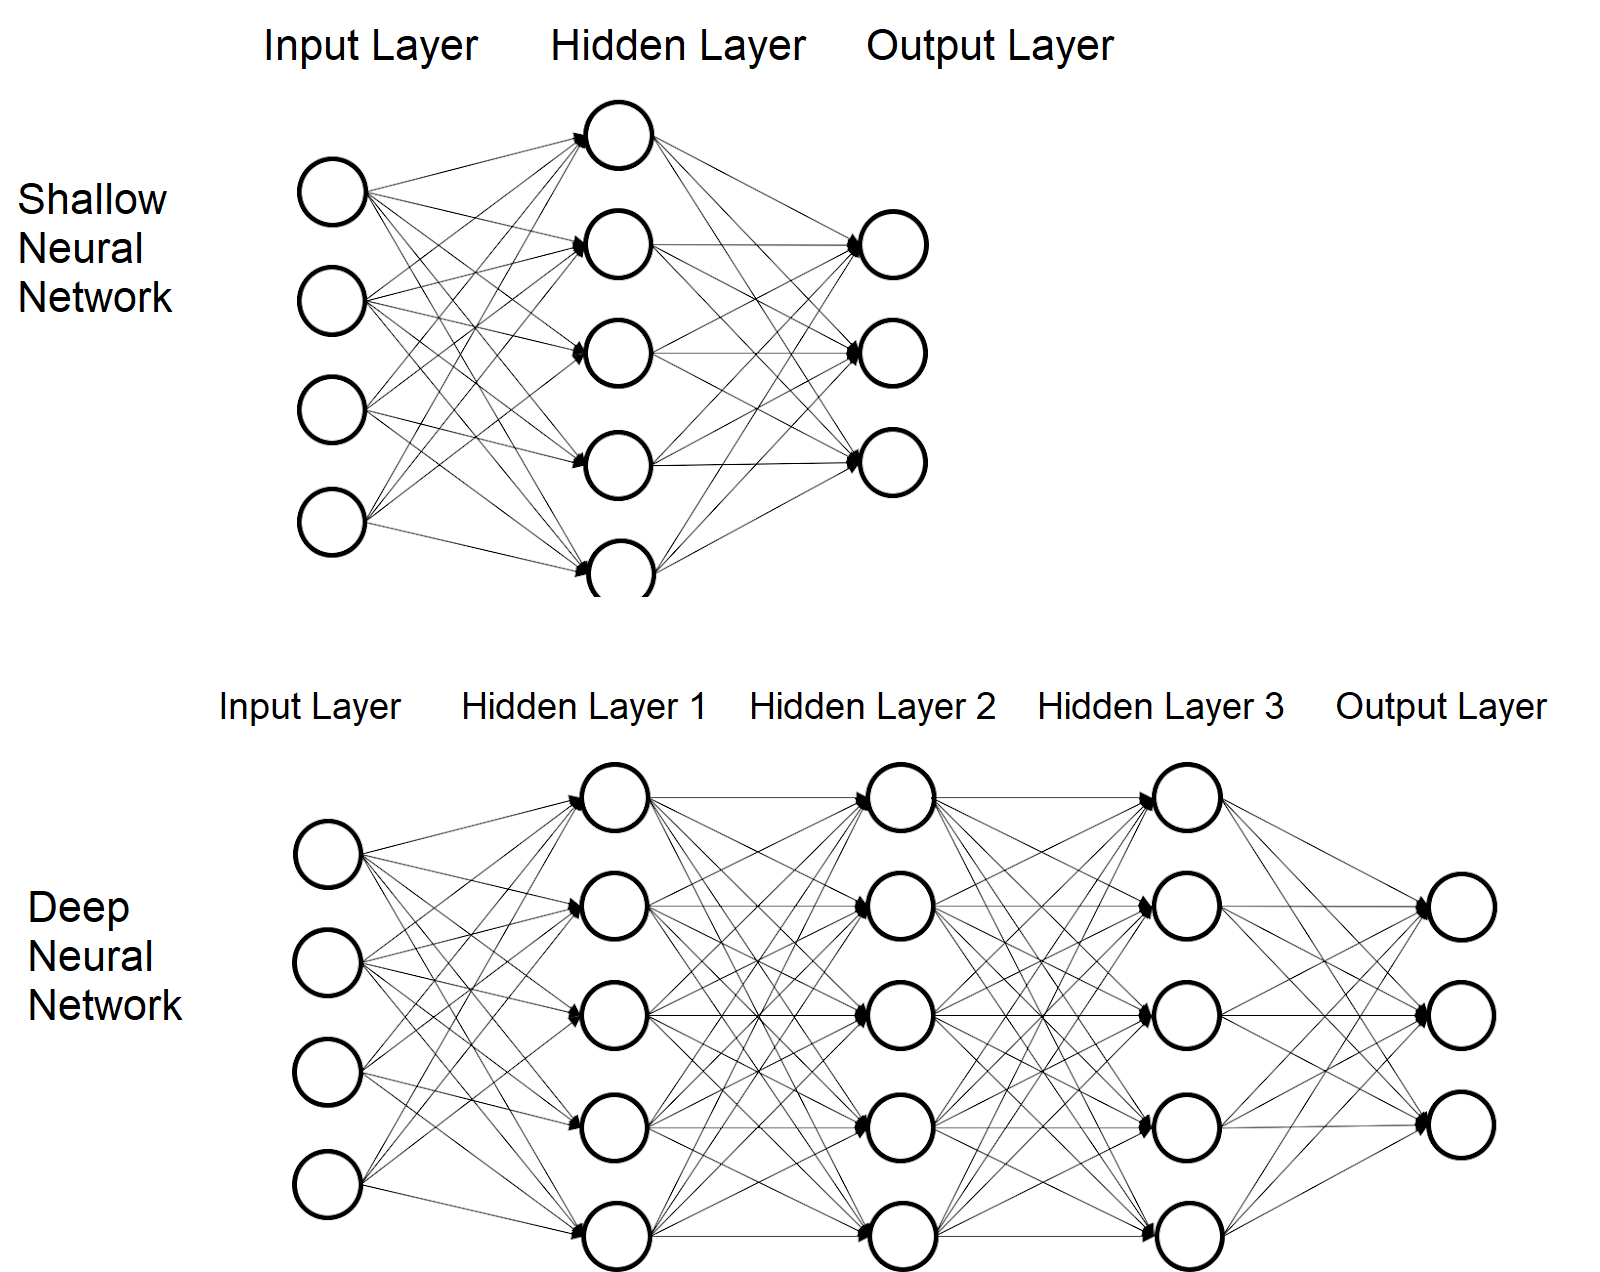
\includegraphics[width=0.7\textwidth]{img/DNN.png}
    \caption{Shallow vs Deep Neural Networks}
    \label{fig:shallow-deep-NN}
\end{figure}

\subsection{Convolutional Neural Networks}
\label{sub:CNN}
This was first proposed by \cite{fukushima_neocognitron_1988} and used by \cite{lecun_gradient-based_1998} for document recognition. It is very popular for image classification but is also used in Speech technology \cite{abdel-hamid_exploring_2013} \cite{ghahremani_acoustic_2016} \cite{dua_developing_2022}. 

CNNs perform better than DNNs due to the fact that they are highly optimised for processing 2D and 3D features like in images and are effective at learning and extracting of 2D features abstractions. Furthermore, CNNs have far fewer parameters than a similarly sized fully connected network. CNNs are made up of feature extractor and classifier modules. Each network layer in the feature extraction module receives the output from the previous layer as its input and passes it on to the next layer \cite{backstrom_introduction_2022}. %The CNN architecture mainly consists of three types of layers: convolution, pooling, and classification.

\begin{figure}[h!]
    \centering
    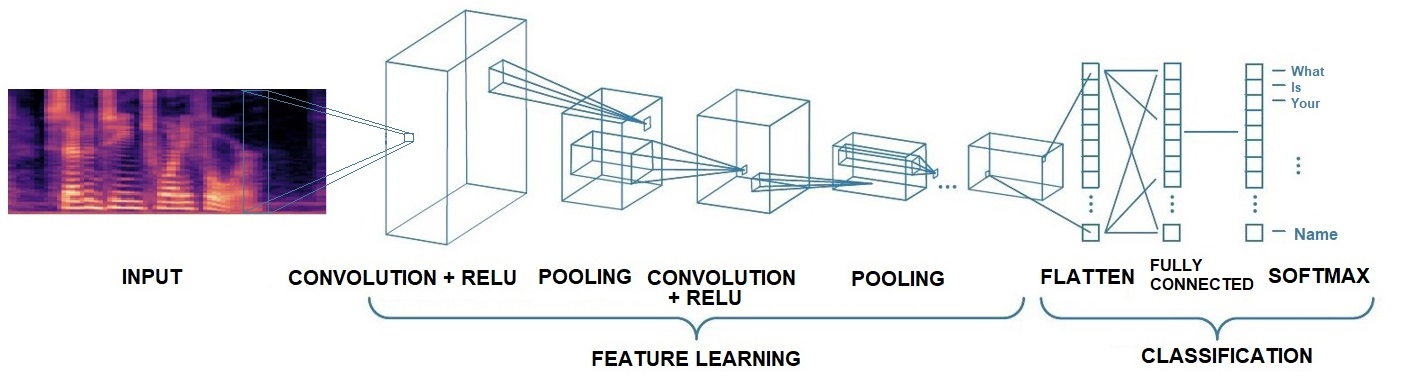
\includegraphics[width=0.95\textwidth]{img/CNN.jpg}
    \caption{CNN Architecture}
    \label{fig:cnn-arch}
\end{figure}

Convolutional Neural Networks consists of mainly following layers \cite{fukushima_neocognitron_1988}:
\begin{enumerate}
    \item \textbf{Convolutional layer:} A filter scans the image a few pixels at a time, to create a feature map predicting the class each feature belongs to. %Thus the feature mappings from previous layers are convolved with learnable kernels in this layer. To form the output feature maps, the kernel output is passed through a linear or non-linear activation function such as sigmoid, hyperbolic tangent, Softmax, rectified linear, and identity functions. Each output feature map can be combined with multiple input feature maps.
    \item \textbf{Pooling layer:} It preserves the most crucial information while reducing the amount of information in each feature obtained from convolution layers. There are typically several convolution and pooling rounds.
    \item \textbf{Fully connected input layer:} It flattens the output of the preceding layers into a single vector that can be used as an input for the following layer.
    \item \textbf{The first fully connected layer:} It applies weights to the feature analysis inputs in order to predict the right label.
    \item \textbf{Fully connected output layer:} Provides the final probabilities for each label.
\end{enumerate}

Higher-level audio features in CNNs are derived from lower-level layer features. As the convolution and pooling operations propagate to the highest layer or level, the dimensions of the features decrease depending on the size of the kernel. To ensure classification accuracy, the number of feature maps typically rises in order to represent the input images' better features. A fully connected network receives its input from the CNN's final layer of output. Since they perform better, feed-forward neural networks are utilised as the classification layer \cite{abdel-hamid_exploring_2013}.

CNNs performance depends on multiple hyper parameters like number of layers, number of feature maps in each layer, the use of dropouts, batch normalization, etc which is why the model must be fine-tuned on the hyper-parameters by conducting multiple experiments to find the right setting of hyper-parameters values after which the model is trained for for a certain given number of epochs \cite{backstrom_introduction_2022}.

\subsection{TDNN}

\begin{figure}[htb]
    \centering
    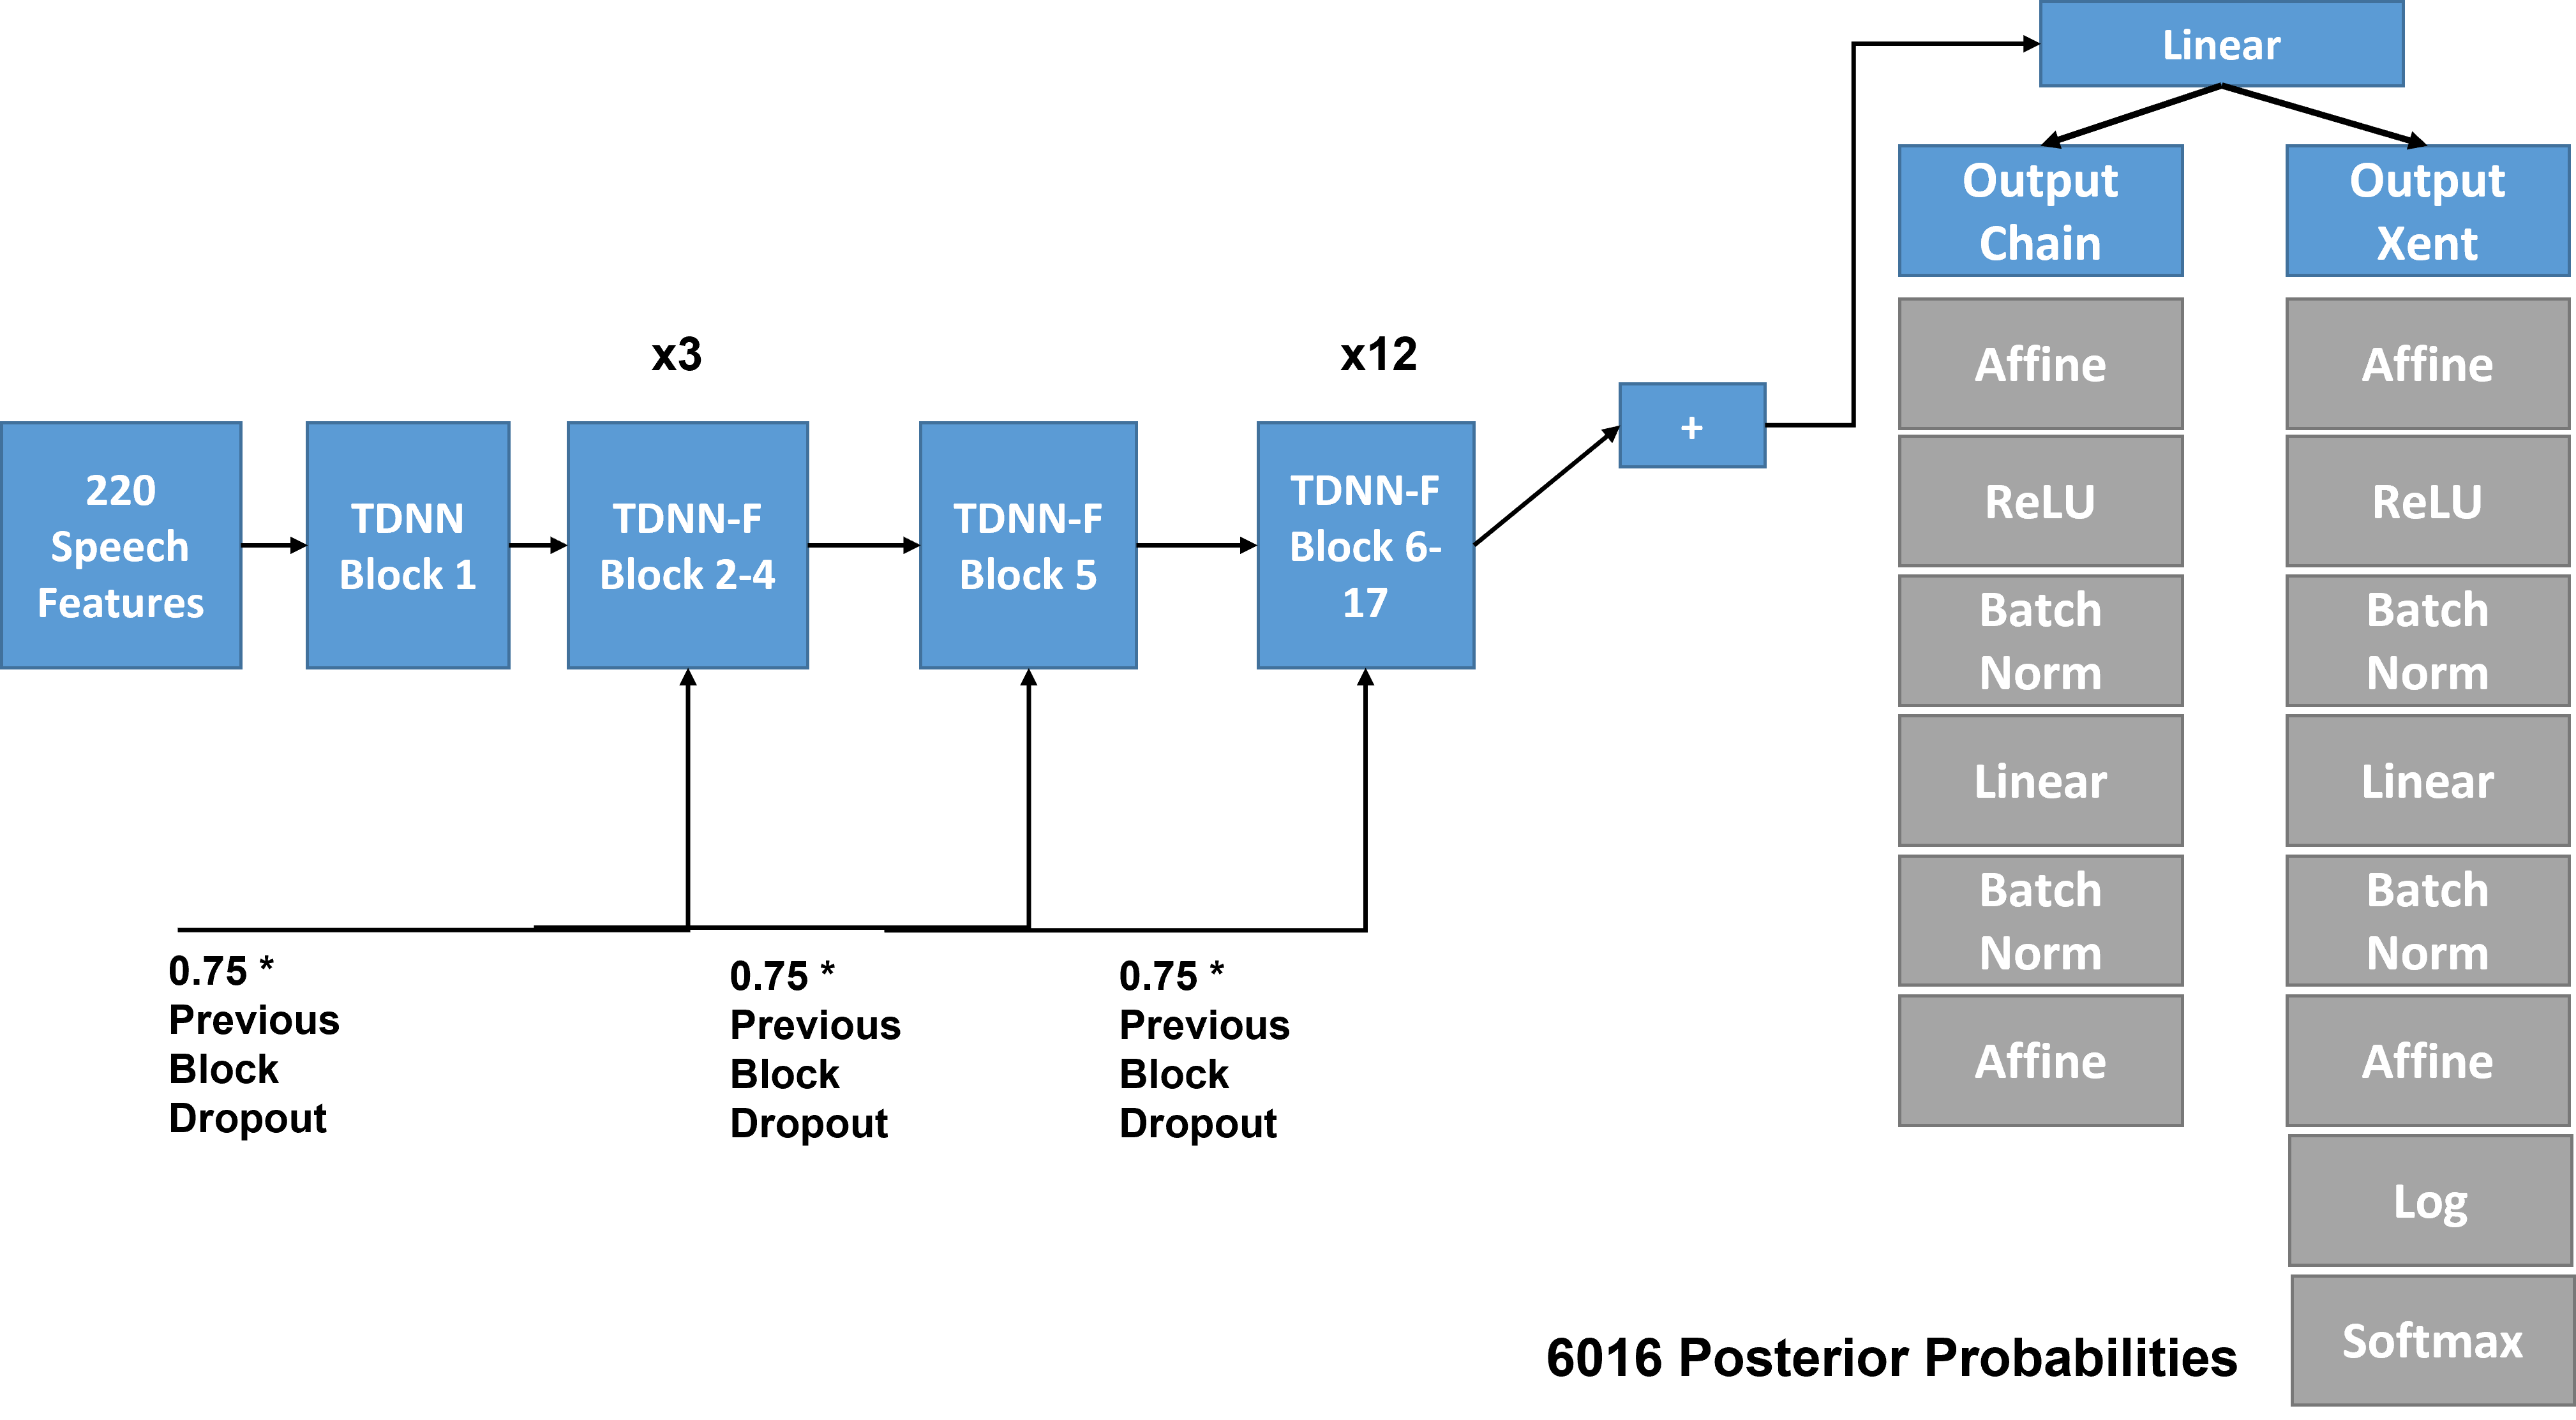
\includegraphics[width=0.9\textwidth]{img/TDNN2.png}
    \caption{TDNN Architecture Basic Layout}
    \label{fig:TDNN-arch}
\end{figure}

Time-Delay Neural Network (TDNN), originally invented by Alex Waibel and Geoffrey Hinton, captures long term temporal correlations between speech frames i.e they are time-dilated 1-Dimensional CNNs. It is a time-domain convolutional network that models temporal dependencies which is easier to parallelize in contrast to a recurrent network and is comparable to feed-forward DNN in terms of training time \cite{noauthor_tdnn_nodate}. It has special characteristics of shift in-variance just like CNN. TDNN can learn short intervals contexts between input features like MFCC and of longer intervals in upper layers i.e. lower layers learn short input contexts, and higher layers learn long input contexts \cite{liu_time_2019}.

\begin{figure}[h!]
    \centering
    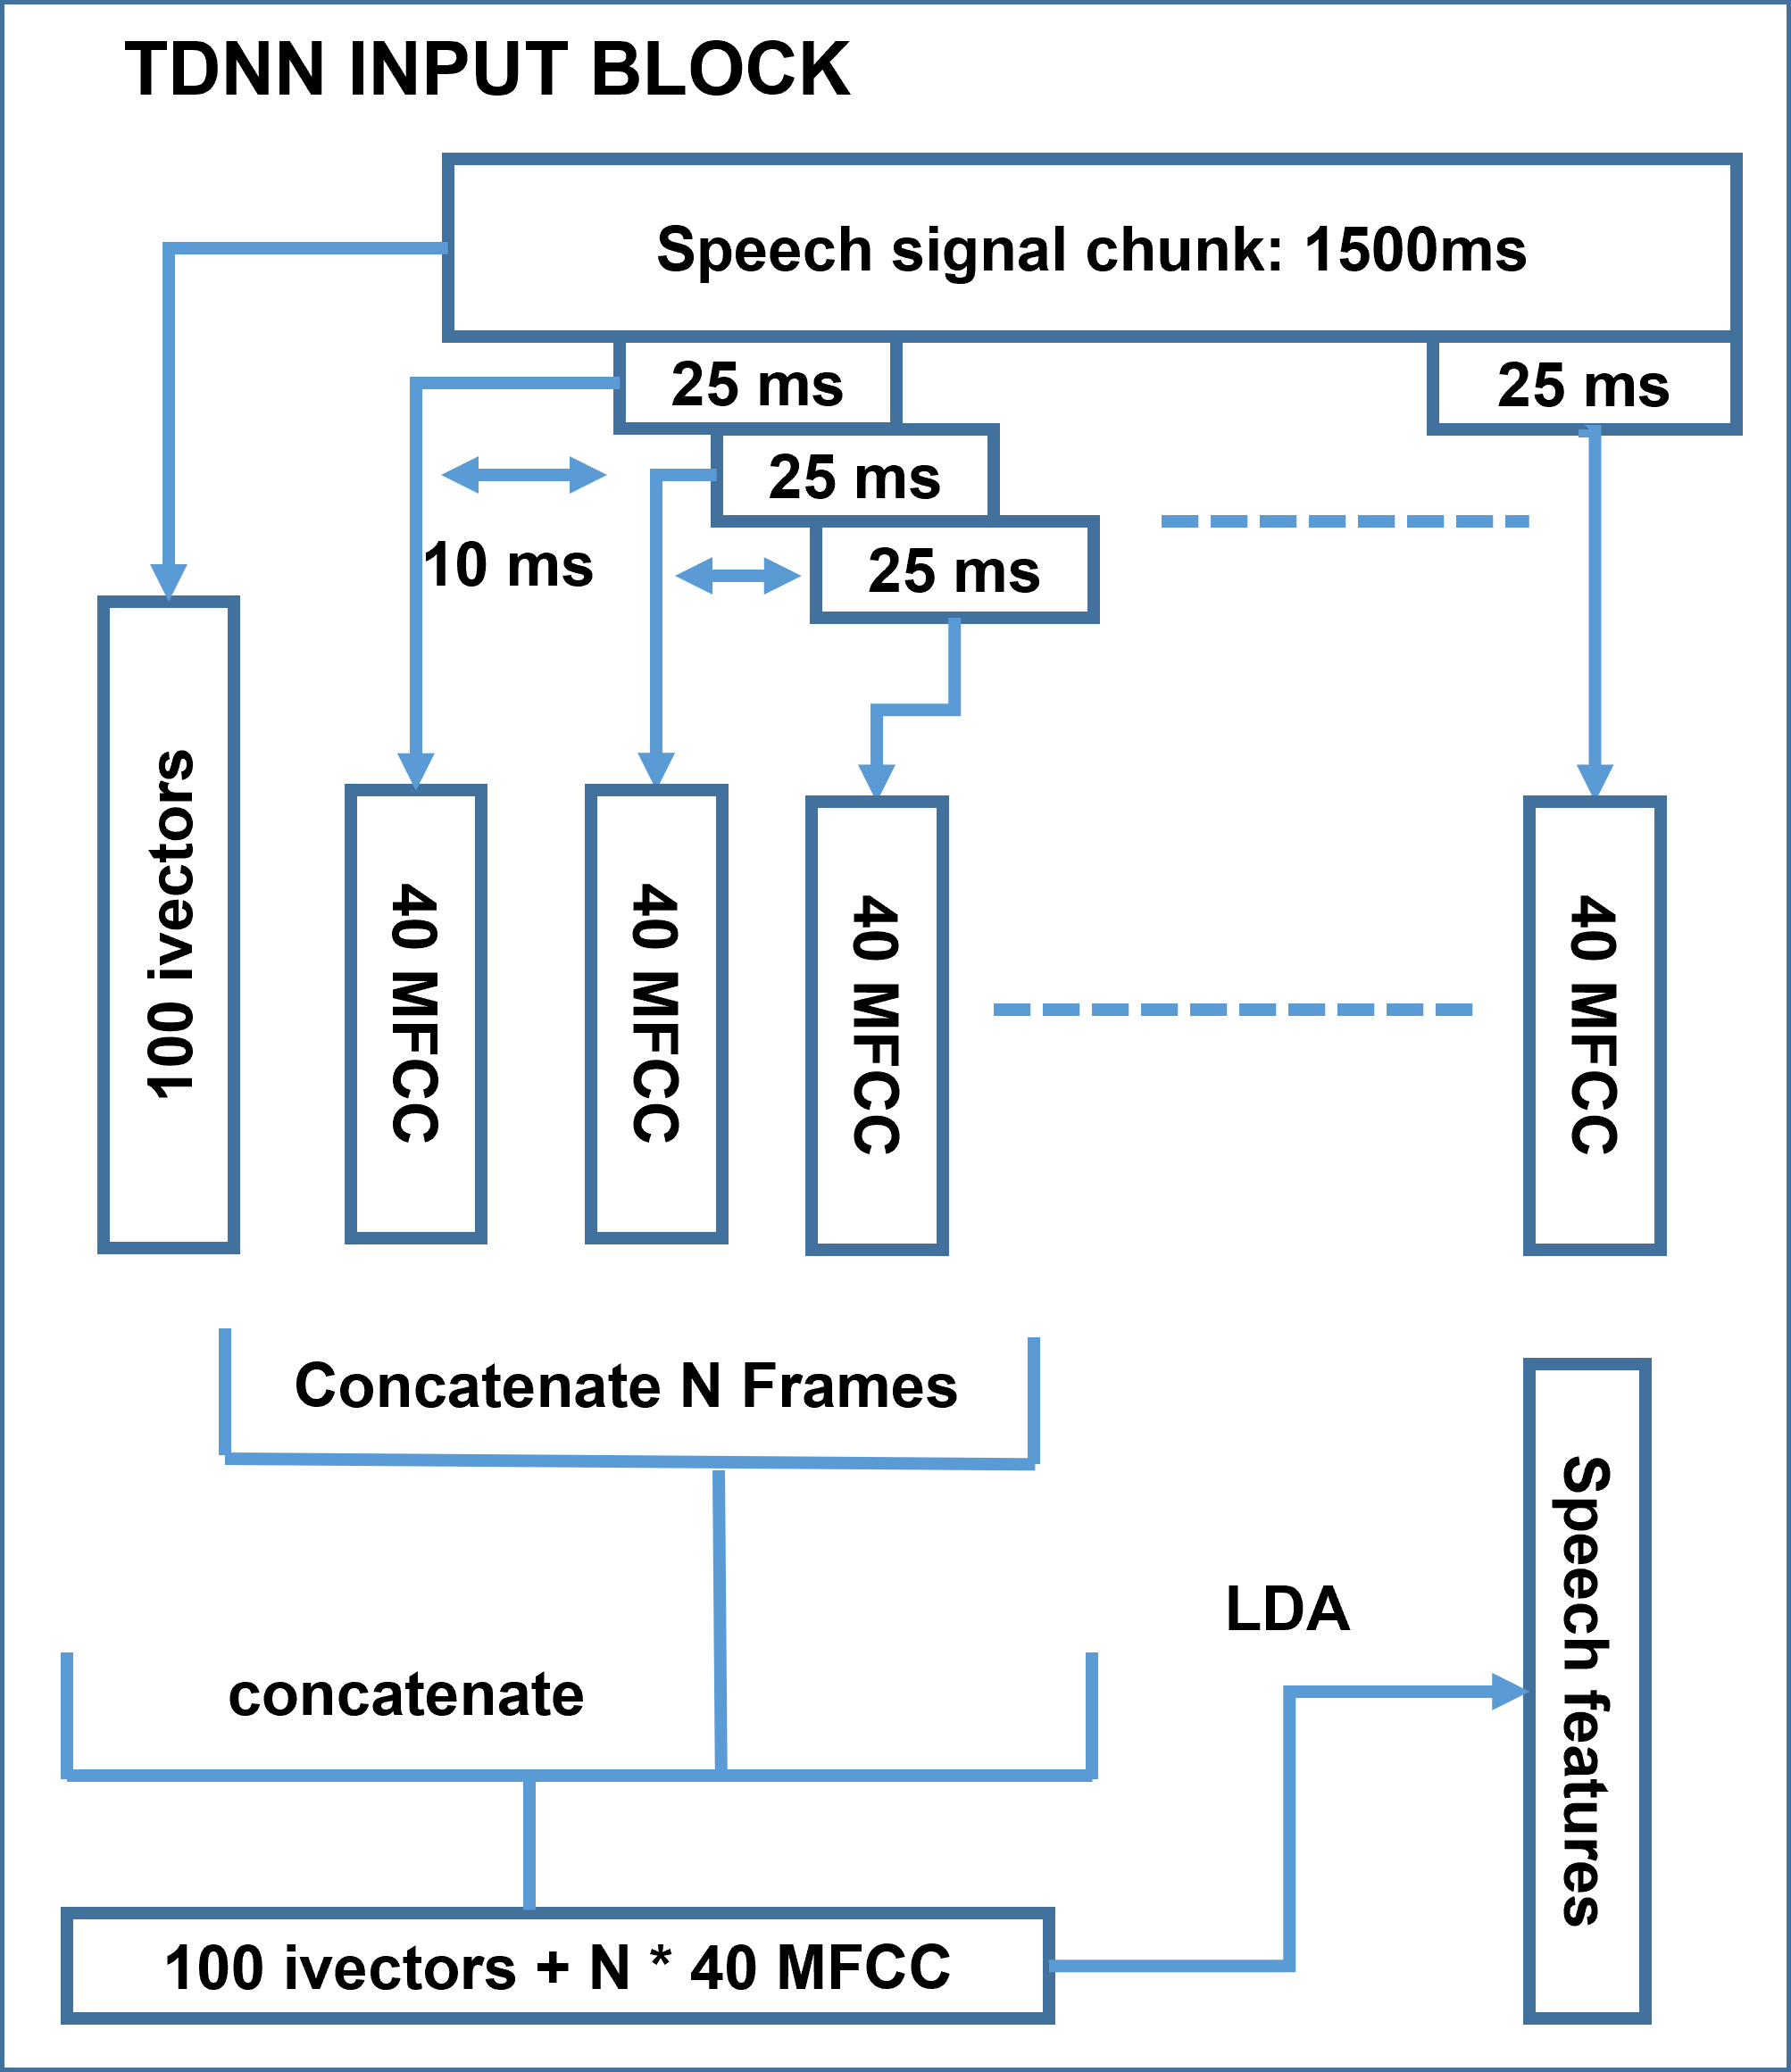
\includegraphics[width=0.4\textwidth]{img/TDNN INPUT.png}
    %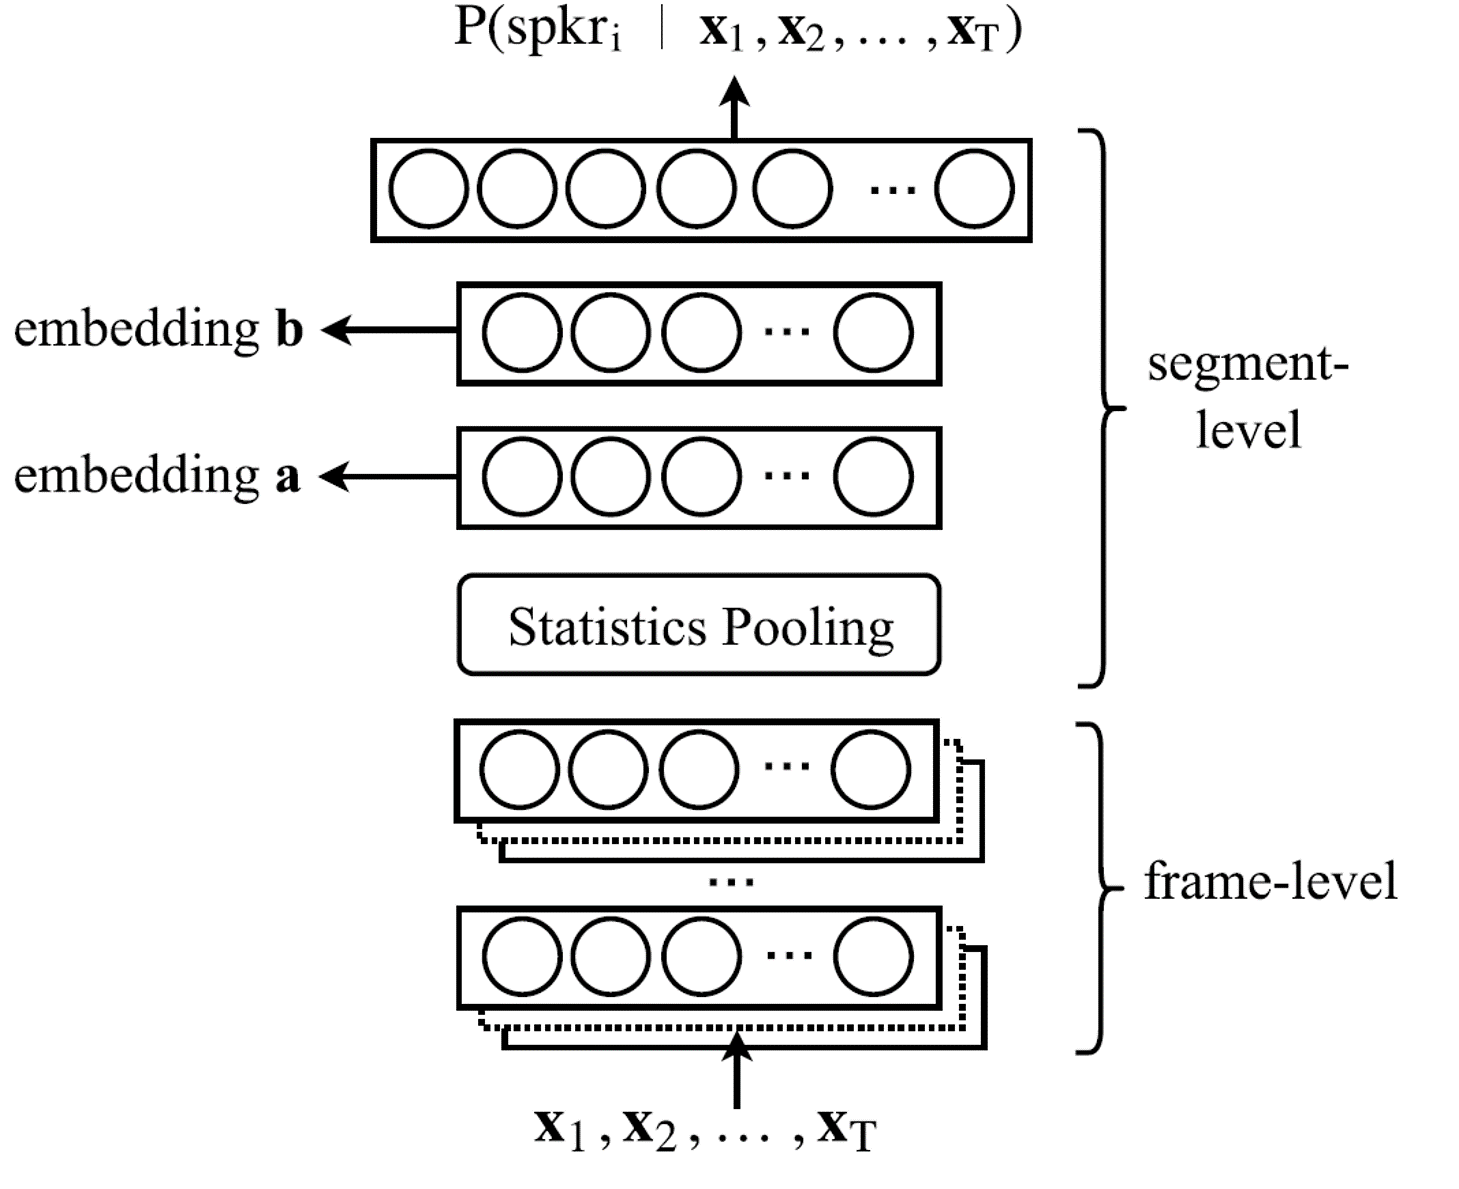
\includegraphics[width=0.4\textwidth]{img/tdDNN frame and segment.png}
    \caption{TDNN Input}   
    \label{fig:TDNN-INPUT}
\end{figure}

Each unit's input is spatially expanded out in a couple of sequential units from the previous TDNN layer. Hence, the lower layers learn a narrow-context and higher layers process a broader temporal-context activations. Each layer's input-context length represents the TDNN hyperparameter \cite{kreyssig_improved_2018}.

All features and frames are correlated in speech. We simply make a 25ms window and take 40 MFCCs of that window or segment. We need previous and next frames to predict next frame in actual. In streaming where we want to predict more on based on past frames instead of future frames, TDNN make better sense \cite{liu_time_2019}. 

\begin{figure}[h!]
    \centering
    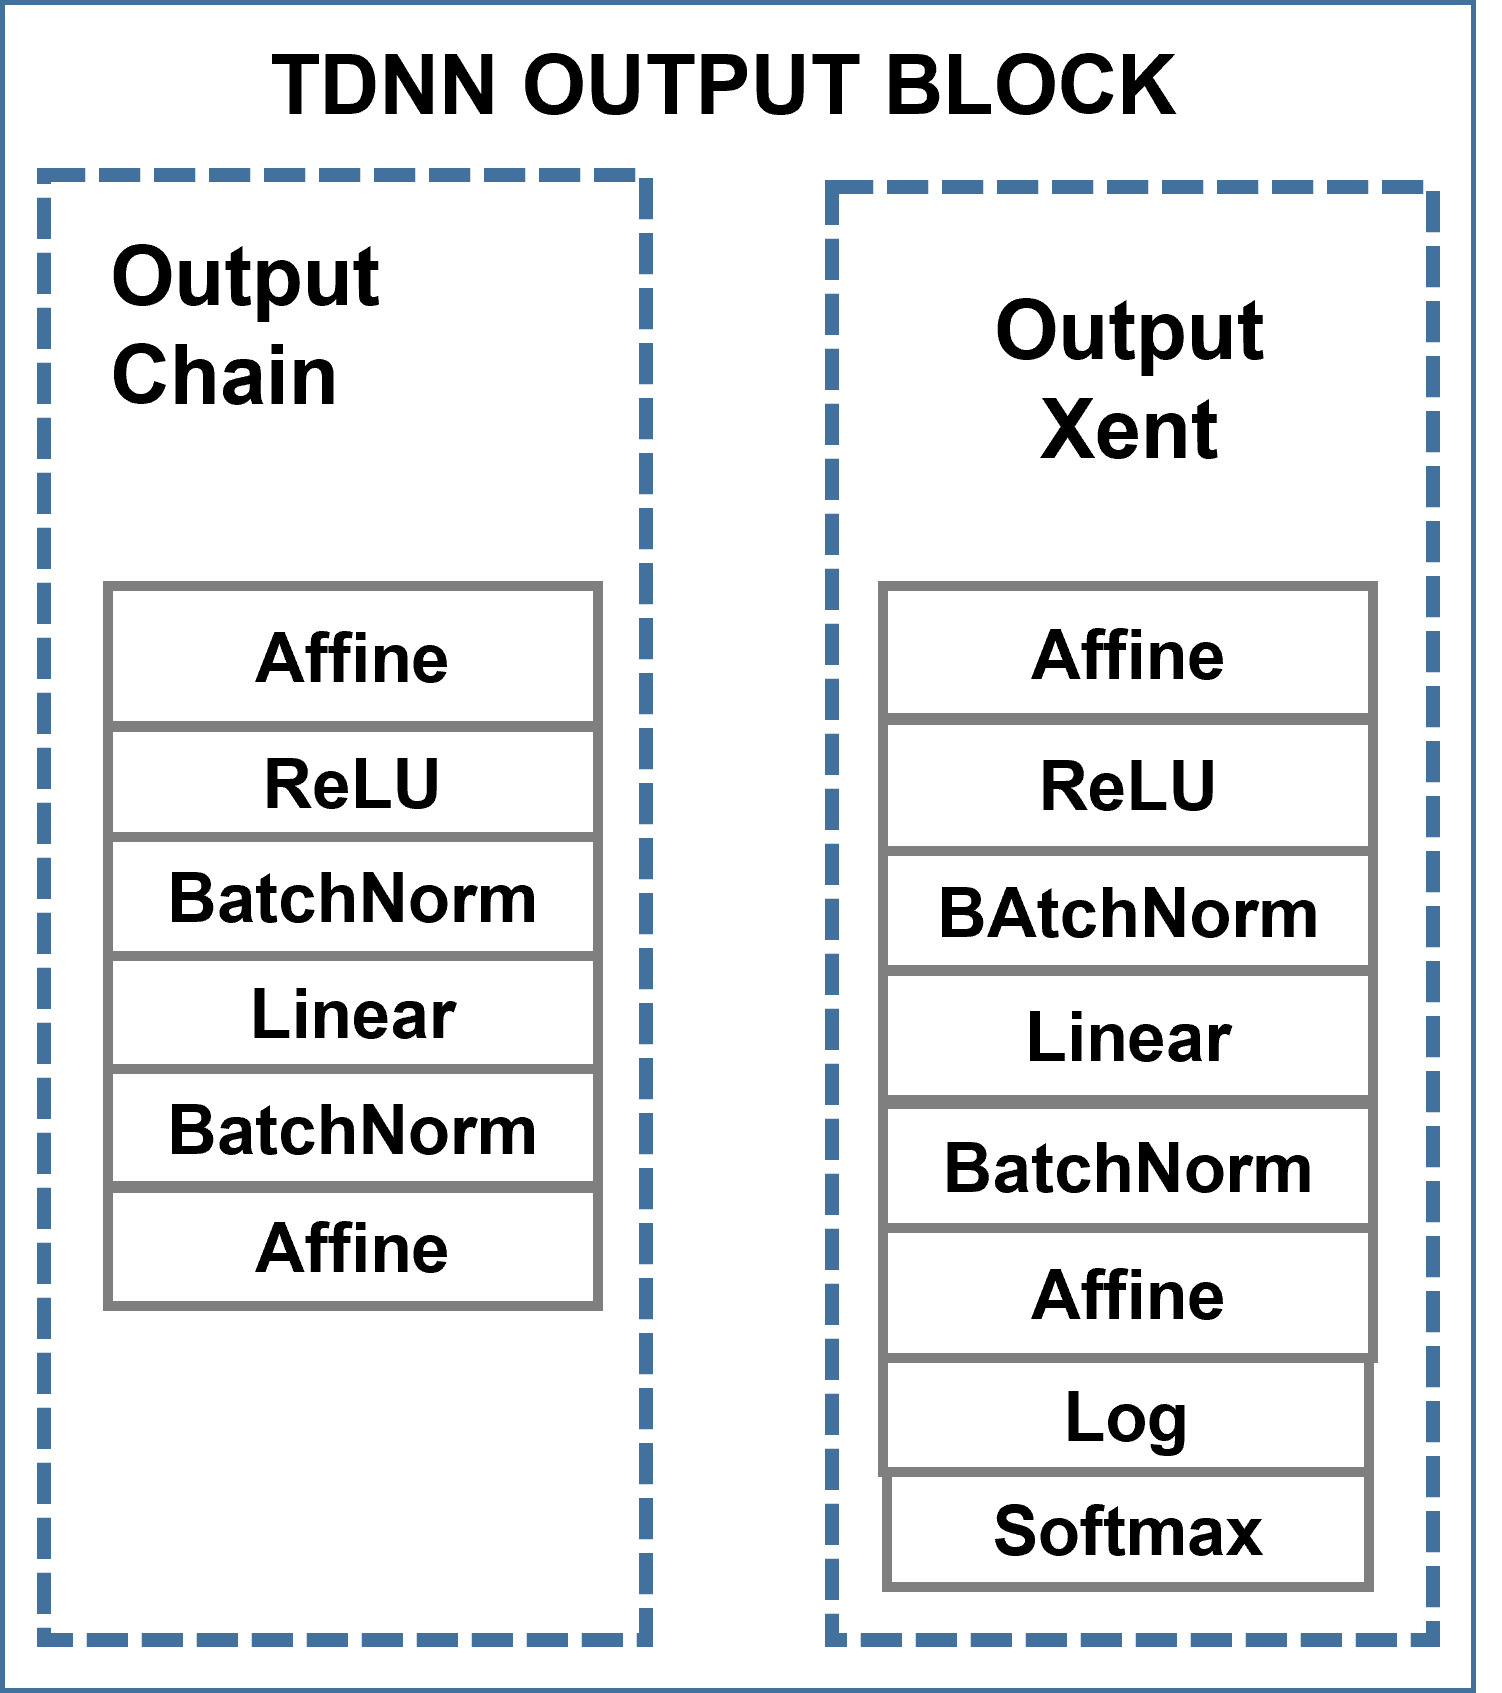
\includegraphics[width=0.3\textwidth]{img/TDNNOUTPUT.png}
    \caption{TDNN Output Block}
    \label{fig:TDNN-OUTPUT-BLOC}
\end{figure}

%\begin{figure}[h!]
%    \centering
%    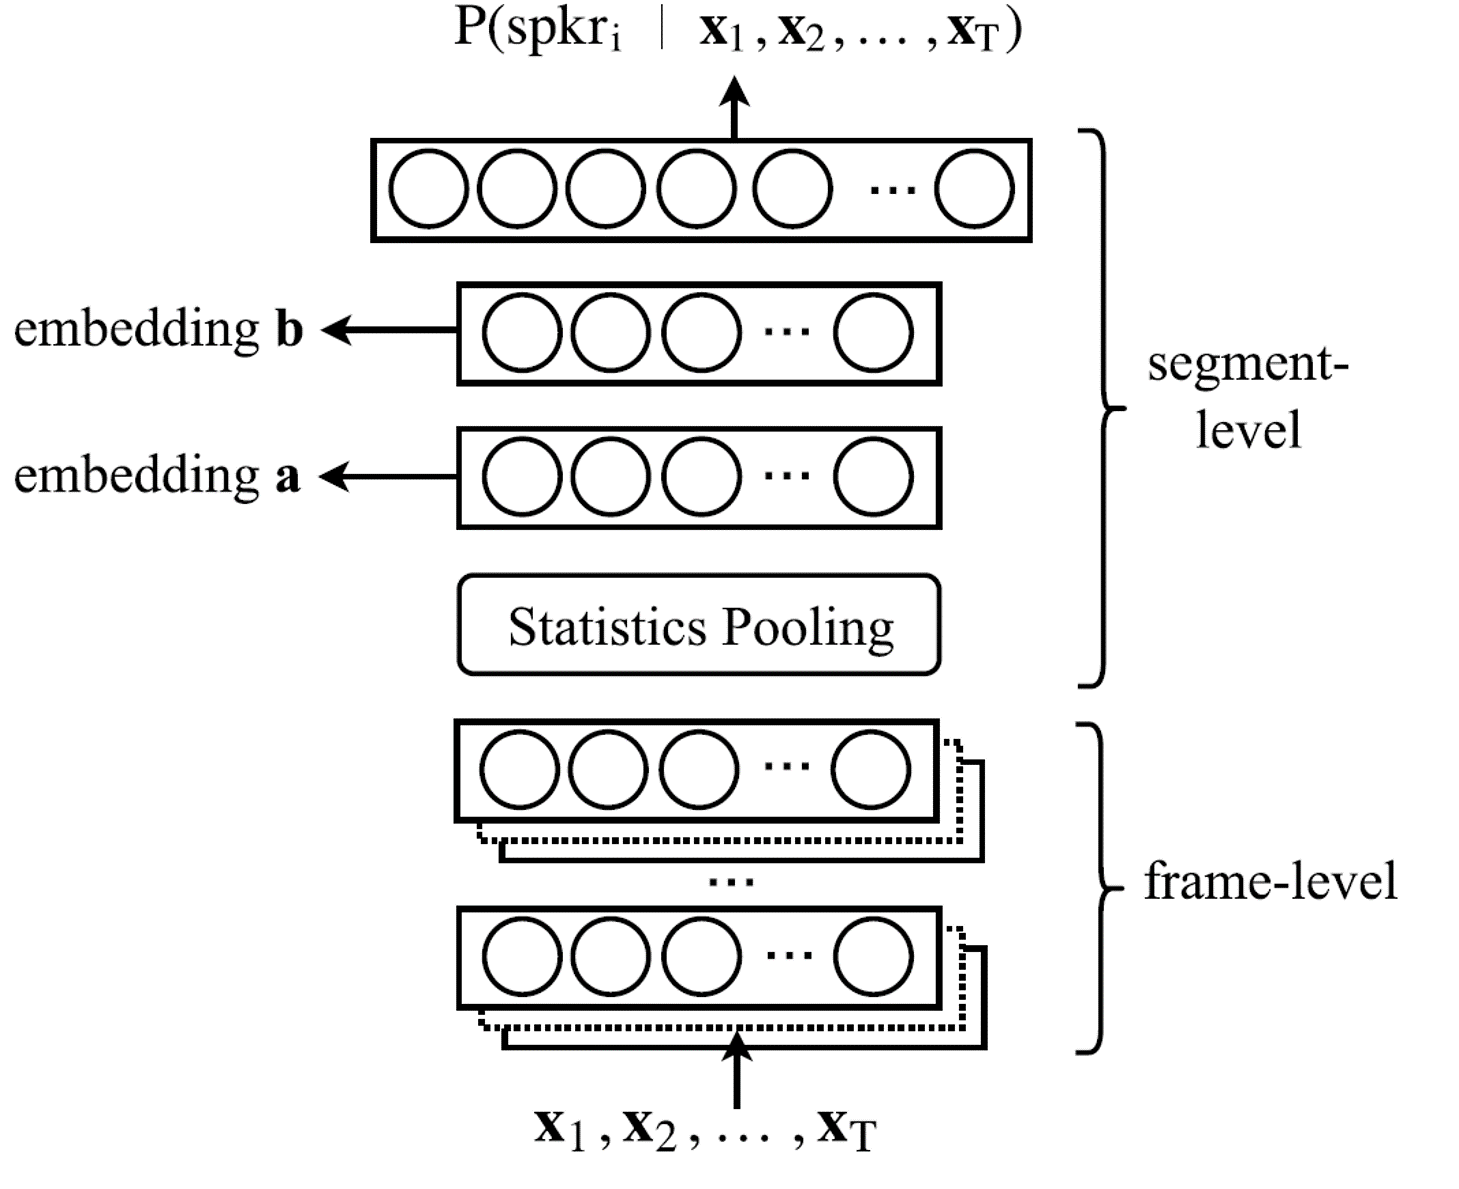
\includegraphics[width=0.5\textwidth]{img/tdDNN frame and segment.png}
%    \caption{TDNN Layers at frame and segment level}
%    \label{fig:TDNN Layers}
%\end{figure}

Input patches consist of fixed number of feature vectors as input to which processes them with fixed local temporal context. The context width increases as we go to upper layers. Finally the last layer representation is pooled by statistics pool layer. The network consist of TDNN which operates at frame level. The last layer output representations from TDNN goes to Statistics pooling layer at every time step. Statistic pool layer computes mean and standard vectors for all the representations from frame 1 to T. Finally these pooled representation goes to next layer which applies affine transformation followed by softmax which can be used for Speech to text of identifying speakers \cite{liu_time_2019}. 

The TDNN architecture is learned on narrow contexts and the upper layers of the networks process wider contexts of the input features, whereas the general Feed Forward Neural Network learns entire input features for processing contexts. Each TDNN layer is updated by a different resolution, which increases as the network layers. By removing duplicated weights from the networks, the TDNN is optimised. A standard Feed Forward Neural learns overlapping features, and removing these duplicated updates reduces training time \cite{yeh_taiwanese_2020}. 

A subsampling is used to reduce duplicated inputs as shown in \ref{fig:tdnn-subsampling} in which nodes and weights (shown by dashed line) are updated only upon application of sub-sampling. The technique does not connect multiple inputs in a hidden layer by allowing space between frames. Since TDNN has a long context going up to the upper layer, the model can learn all input features if the interval between frames is allowed \cite{ritter_neural_2019}. 

\begin{figure}[h!]
    \centering
    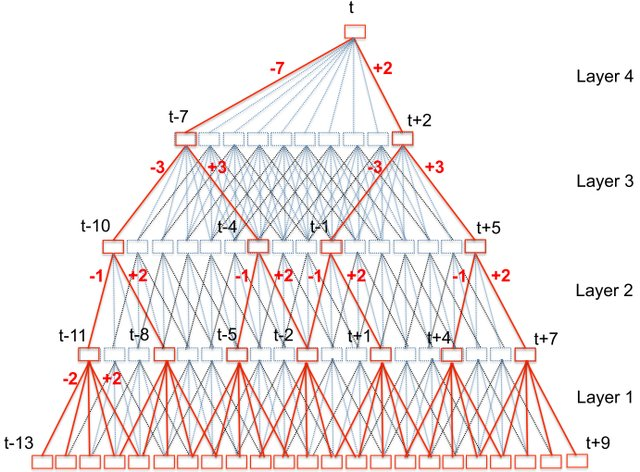
\includegraphics[width=0.8\textwidth]{img/Tdnn-subsampling.jpg}
    \caption{TDNN subsampling \cite{ritter_neural_2019}}
    \label{fig:tdnn-subsampling}
\end{figure}

Furthermore, minimizing the number of edges and nodes in the network reduces the number of parameters that represent the model. Long-term temporal dependencies are better captured by TDNN architecture than by feed-forward DNN. In comparison to baseline DNN model in interactive personal assistant (IPA) domain there is a relative improvement of 7.3\%.  The TDNN is also used to remove reverberation effects in robust acoustic modelling. Using iVectors as input helps TDNN to perform instantaneous speaker and environment adaptation potentially improving 10\% WER \cite{yeh_taiwanese_2020}.

Increasing TDNN layers enables the network to capture features for a longer time period. Deepening the number of network layers of TDNN helps yield better results. However, deeper network tends to cause degradation, hence, the increasing depth of the neural network reduces accuracy for which a different TDNN architecture is used  in order to achieve better speech recognition performance in which Matrix Factorization training of the network makes neural network training stable \cite{povey_semi-orthogonal_2018}.

\subsection{CNN-TDNN}

CNN-TDNN \cite{ghahremani_acoustic_2016} is a variant of simple TDNN model and it is part of a multi-component system comprising of a hybrid HMM-TDNN based acoustic, phonetic and n-gram language model. It has CNN blocks before the TDNN blocks and takes Mel Filterbanks as input instead of MFCCs. The detailed working of CNN-TDNN is given in Section \ref{sec:LFMMI-chain}.

\begin{figure}[htb]
    \centering
    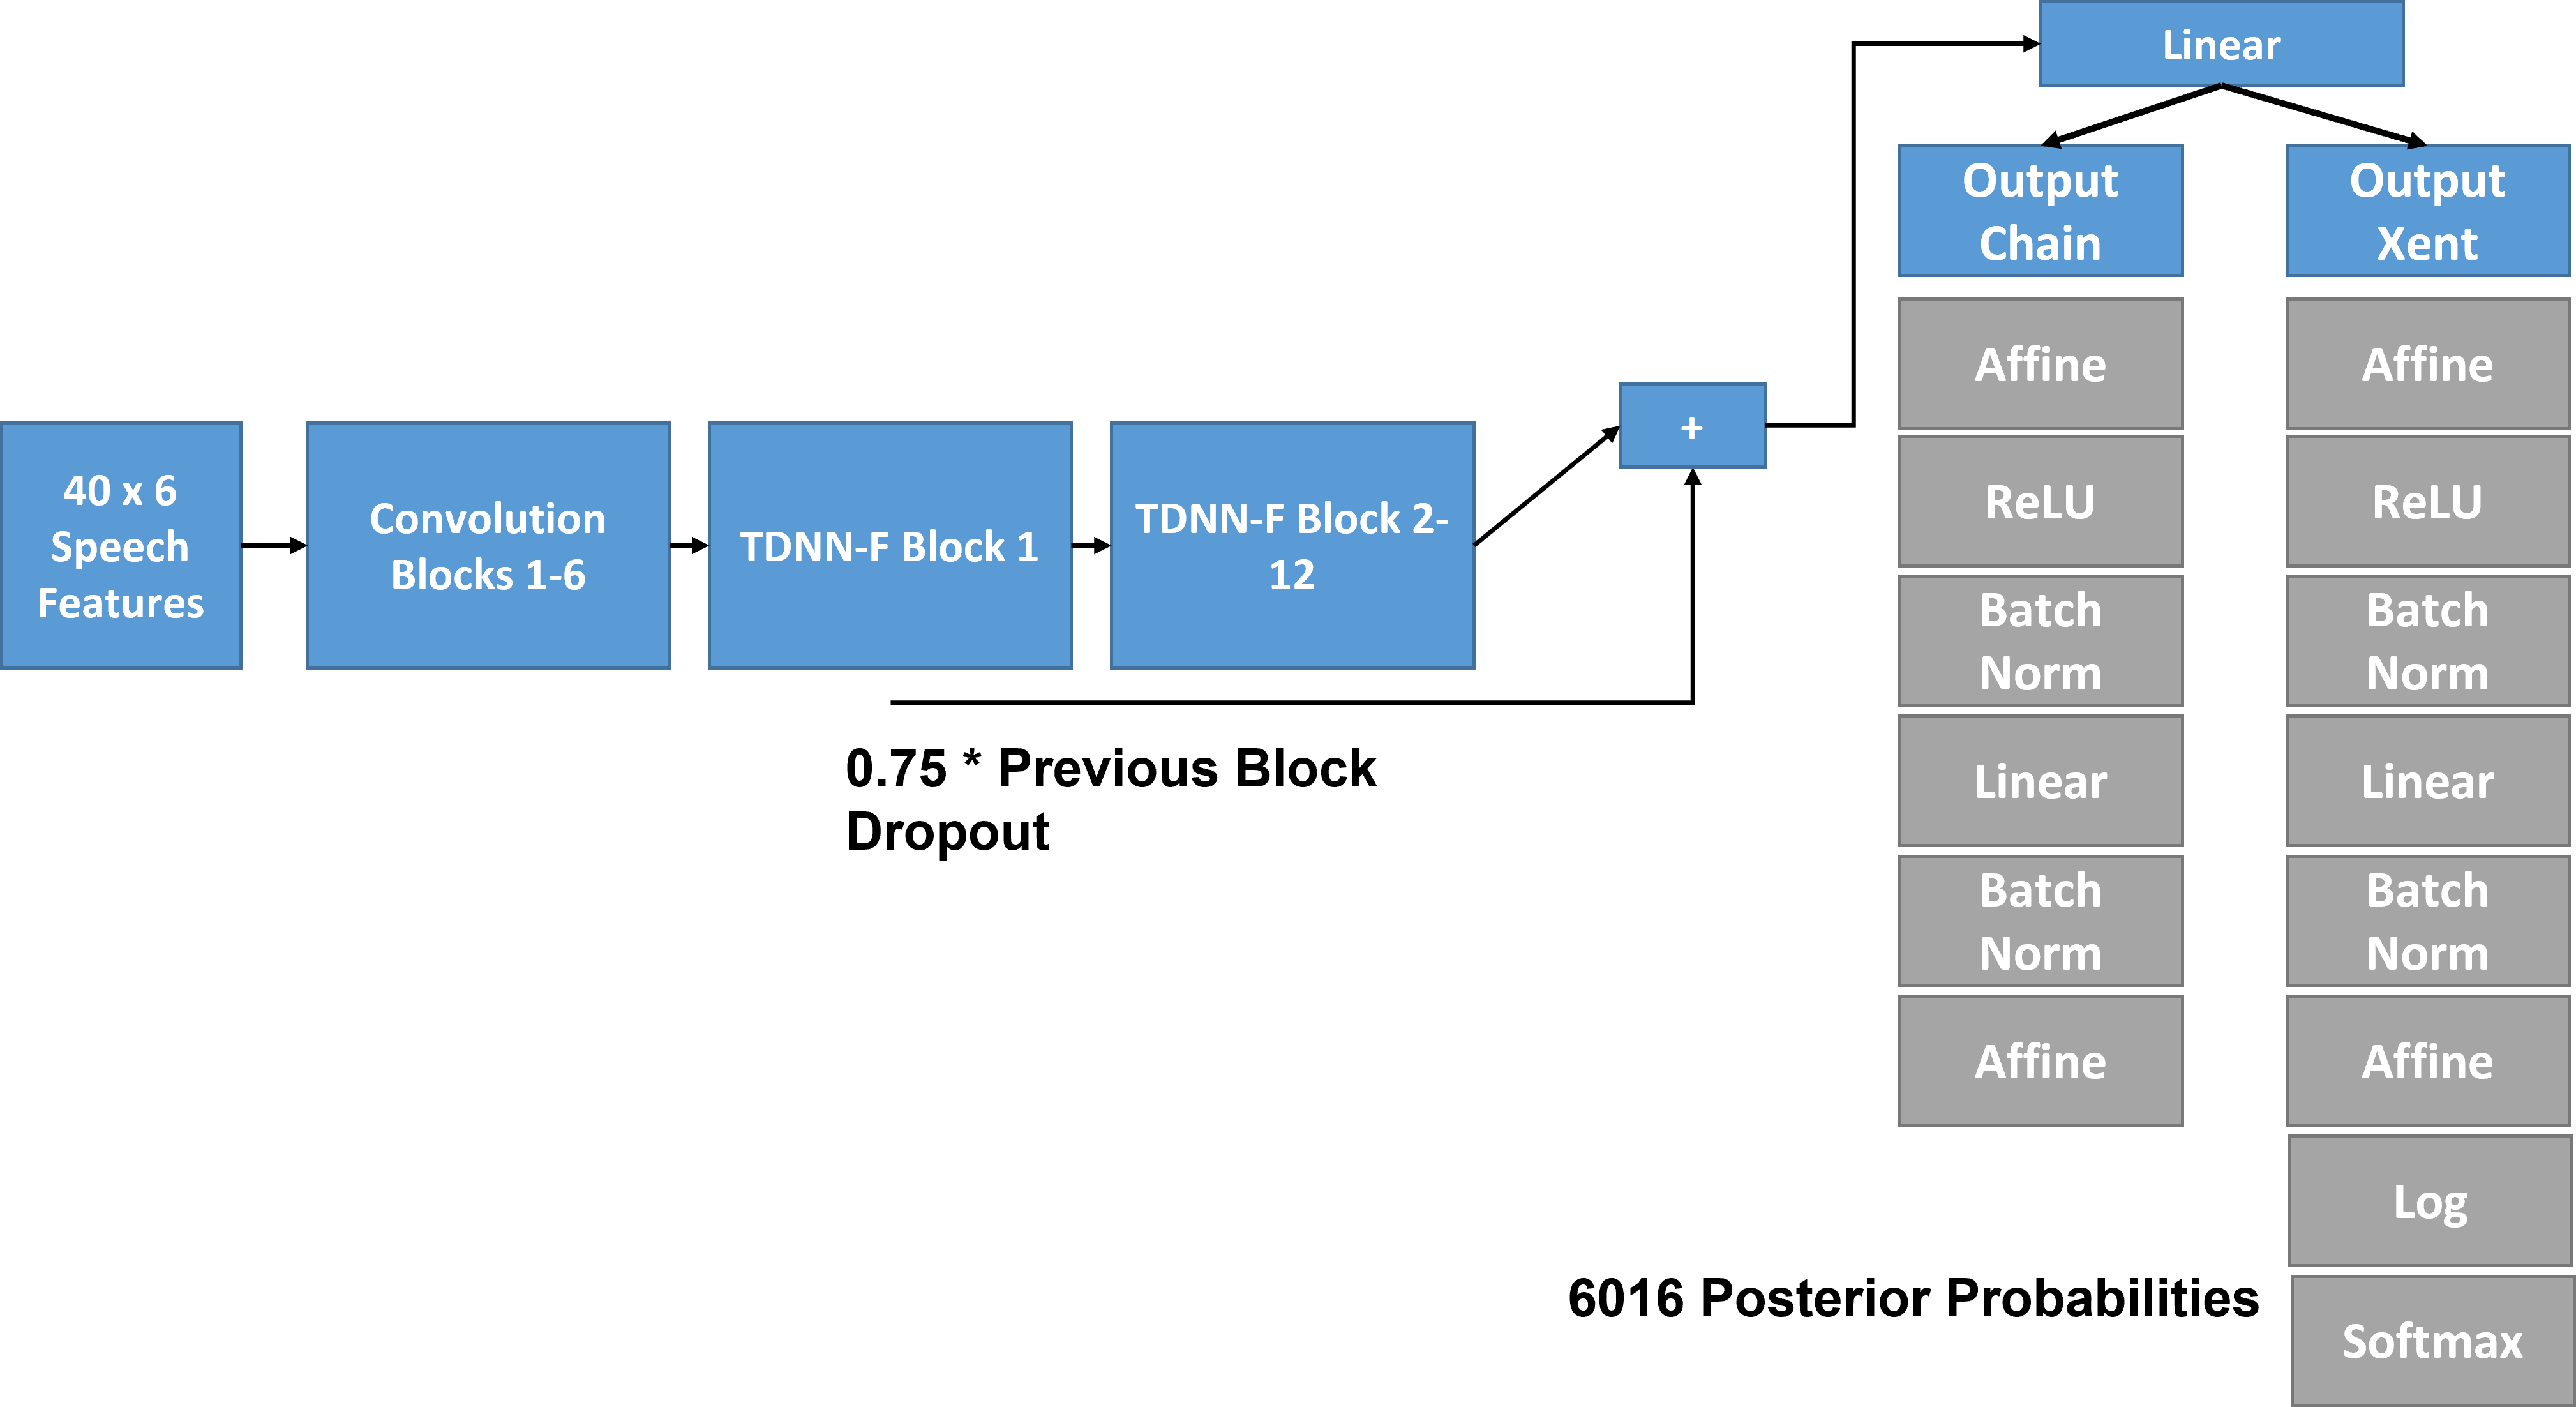
\includegraphics[width=0.7\textwidth]{img/CNNTDNN2.png}
    \caption{CNN-TDNN Basic Layout}
    \label{fig:CNNTDNN-Layout}
\end{figure}

\begin{figure}[h!]
    \centering
    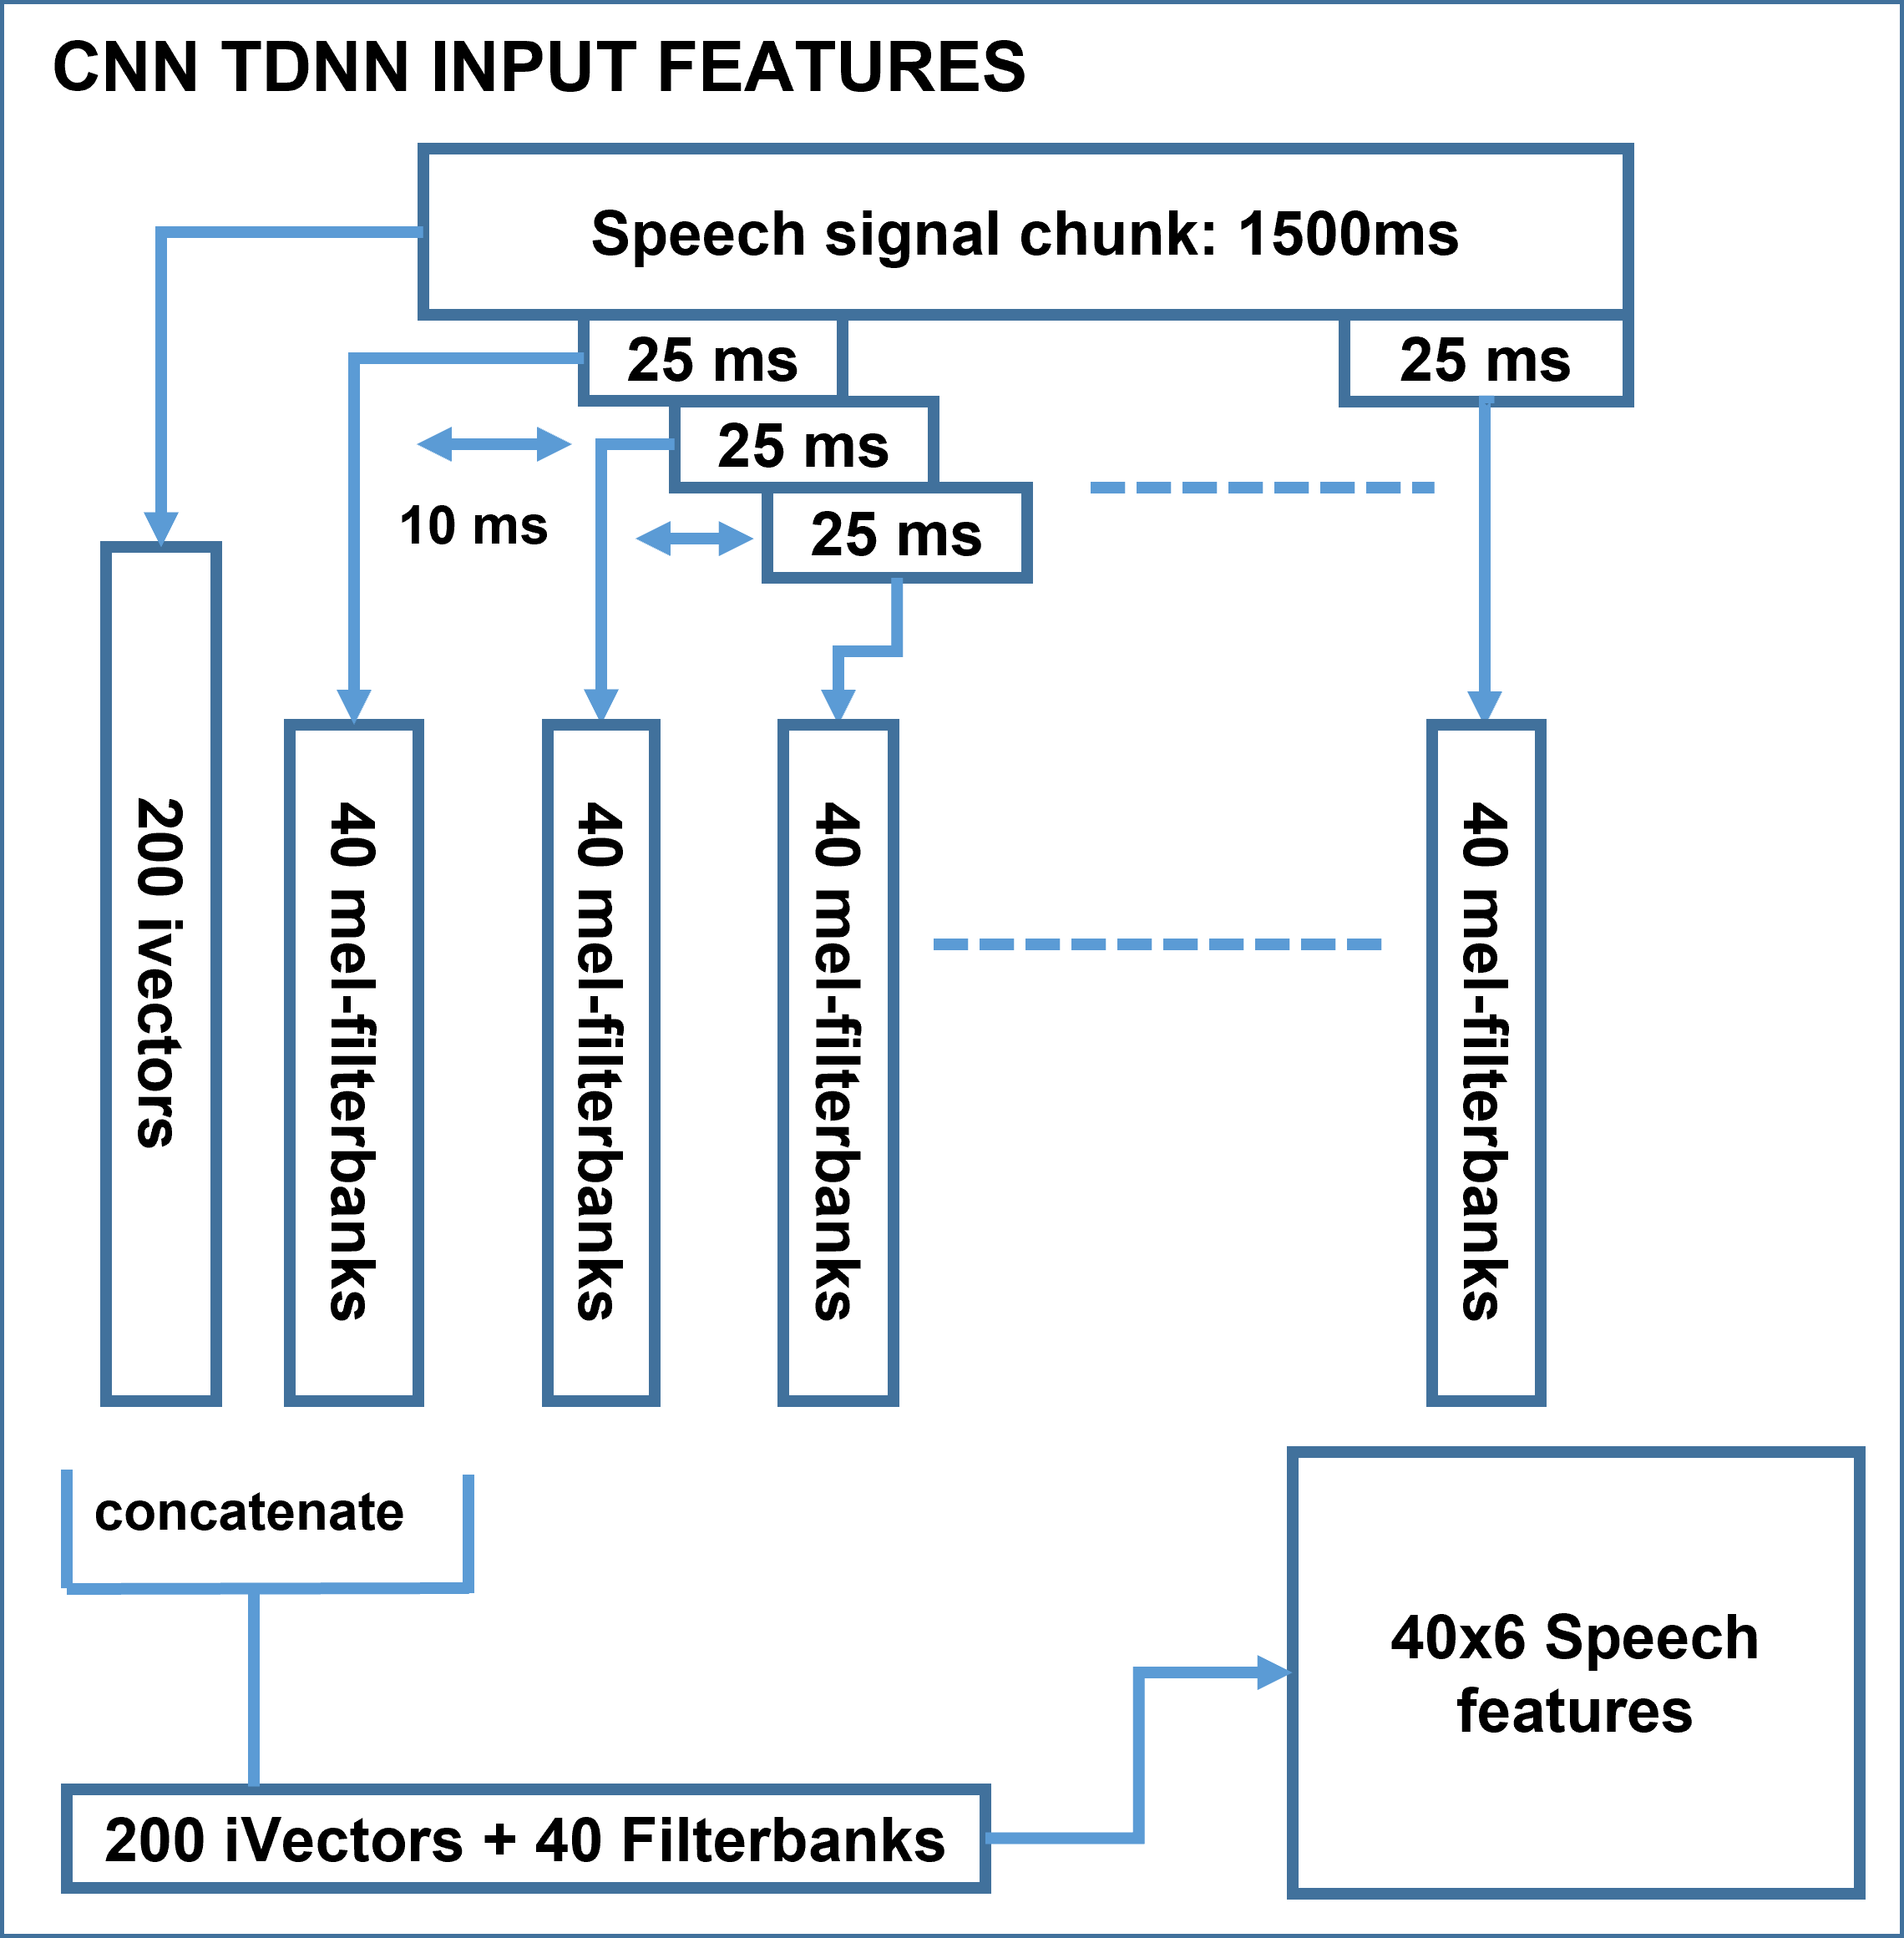
\includegraphics[width=0.4\textwidth]{img/CNNTDNN-INPUT.png}
    \caption{CNN-TDNN Input}
    \label{fig:CNN-TDNN-INPUT}
\end{figure}



\begin{figure}[h!]
    \centering
    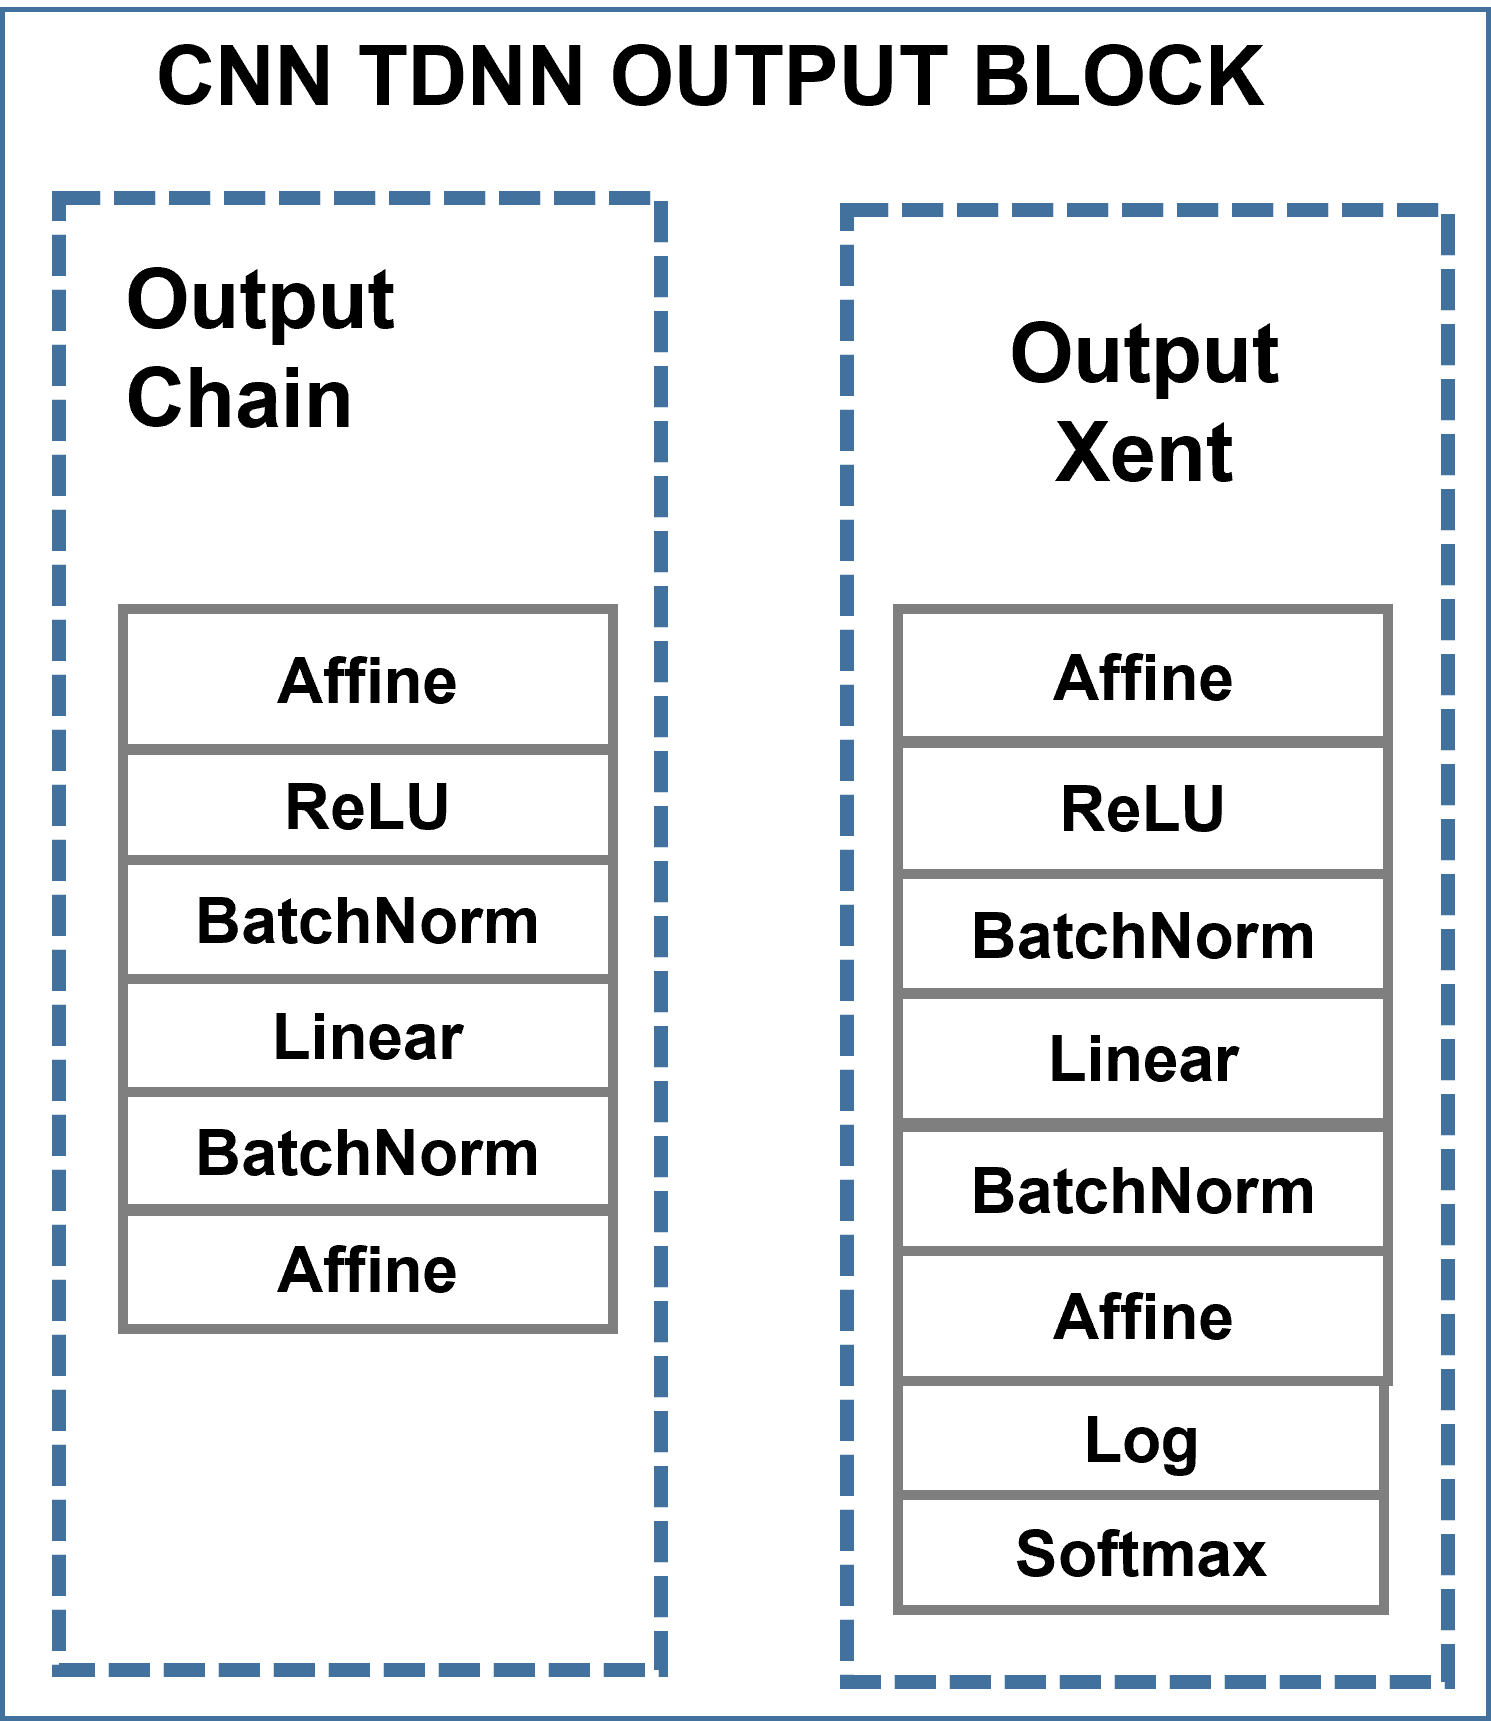
\includegraphics[width=0.4\textwidth]{img/CNNTDNNOUTPUT.png}
    \caption{CNN-TDNN Output}
    \label{fig:CNNTDNN-output}
\end{figure}

%Ghahremani \cite{ghahremani_acoustic_2016} proposed a CNN-TDNN-based raw waveform setup with a repeated network-in-network structure that aggregates time information from convolution filter outputs.

%It introduces Network in Network layer which is a group of micro neural network blocks applied to non-overlapping patches of input with each block being a nonlinear transformation from m dimensional space to n-dimensional space. NIN is a many-to-many non-linearity comprising of two block diagonal matrices, with repeated blocks, inter-leaved between layers of ReLU or Rectified Linear Units. To stabilize training we always add a normalization layer after the NIN non-linearity.

%If the micro neural network block parameters are shared across the NIN, each column of the block $U_{1}$ can be interpreted as a one dimension convolution filter with a filter size \textit{m} and a filter shift \textit{m}. Thus, the same filter is applied to non-overlapping patches and this models local connectivity. The shared parameters in the NIN non-linearity keeps its total parameter count low relative to the size of its input and output, and allows it to be trained faster \cite{ghahremani_acoustic_2016}.

%\begin{figure}[h]
%    \centering
%    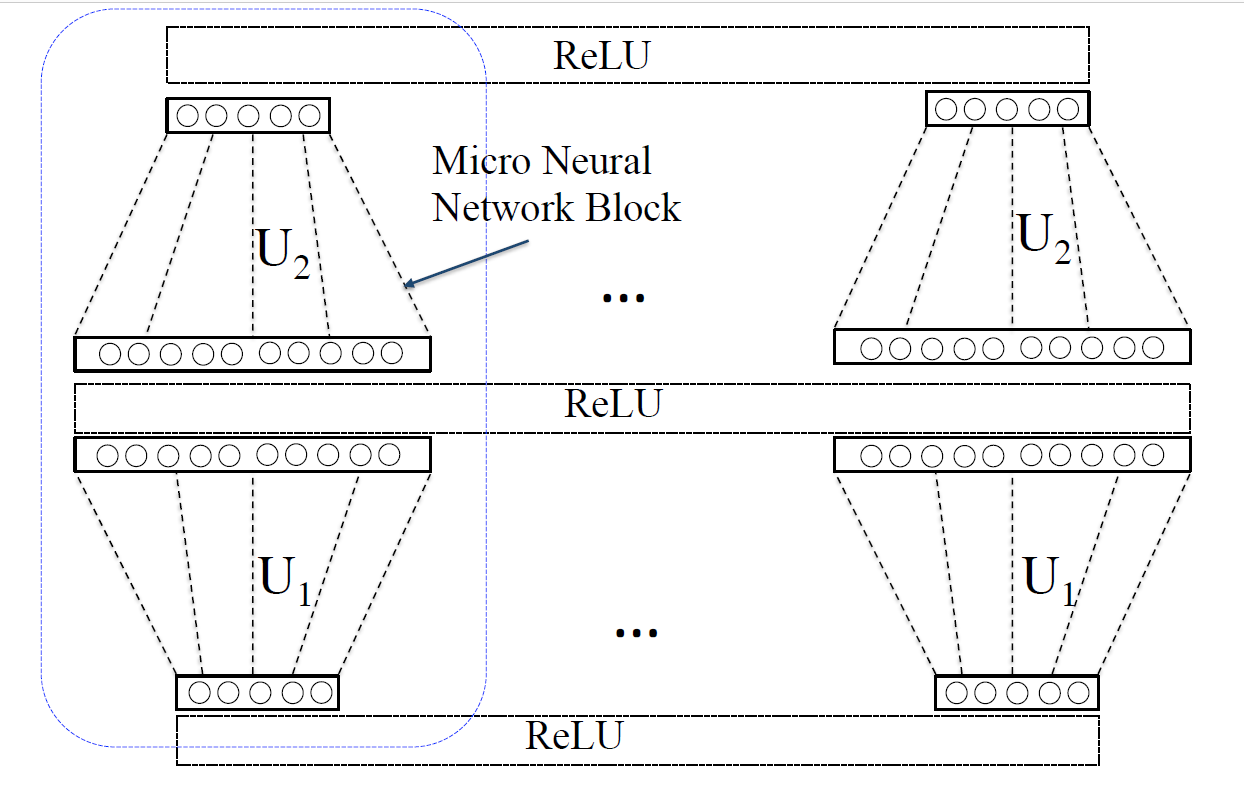
\includegraphics[width=0.6\textwidth]{img/NIN.png}
%    \caption{NIN structure}
%    \label{fig:NIN}
%\end{figure}

%If this Network In Network (NIN) non-linearity replaces the conventional ReLU hidden layer in the DNN, the results improve. 

\section{Training ASRs Completely on Deep Neural Networks}

Due of the shortcomings of the Statistical HMM-based model and coupled with the promotion of deep learning technology, more and more works began to study end-to-end LVCSR. The goal was to bypass the complex structuring of Traditional ASR to achieve a joint language and acoustic model of sorts in one model using Deep Learning.

\begin{figure}[h]
    \centering
    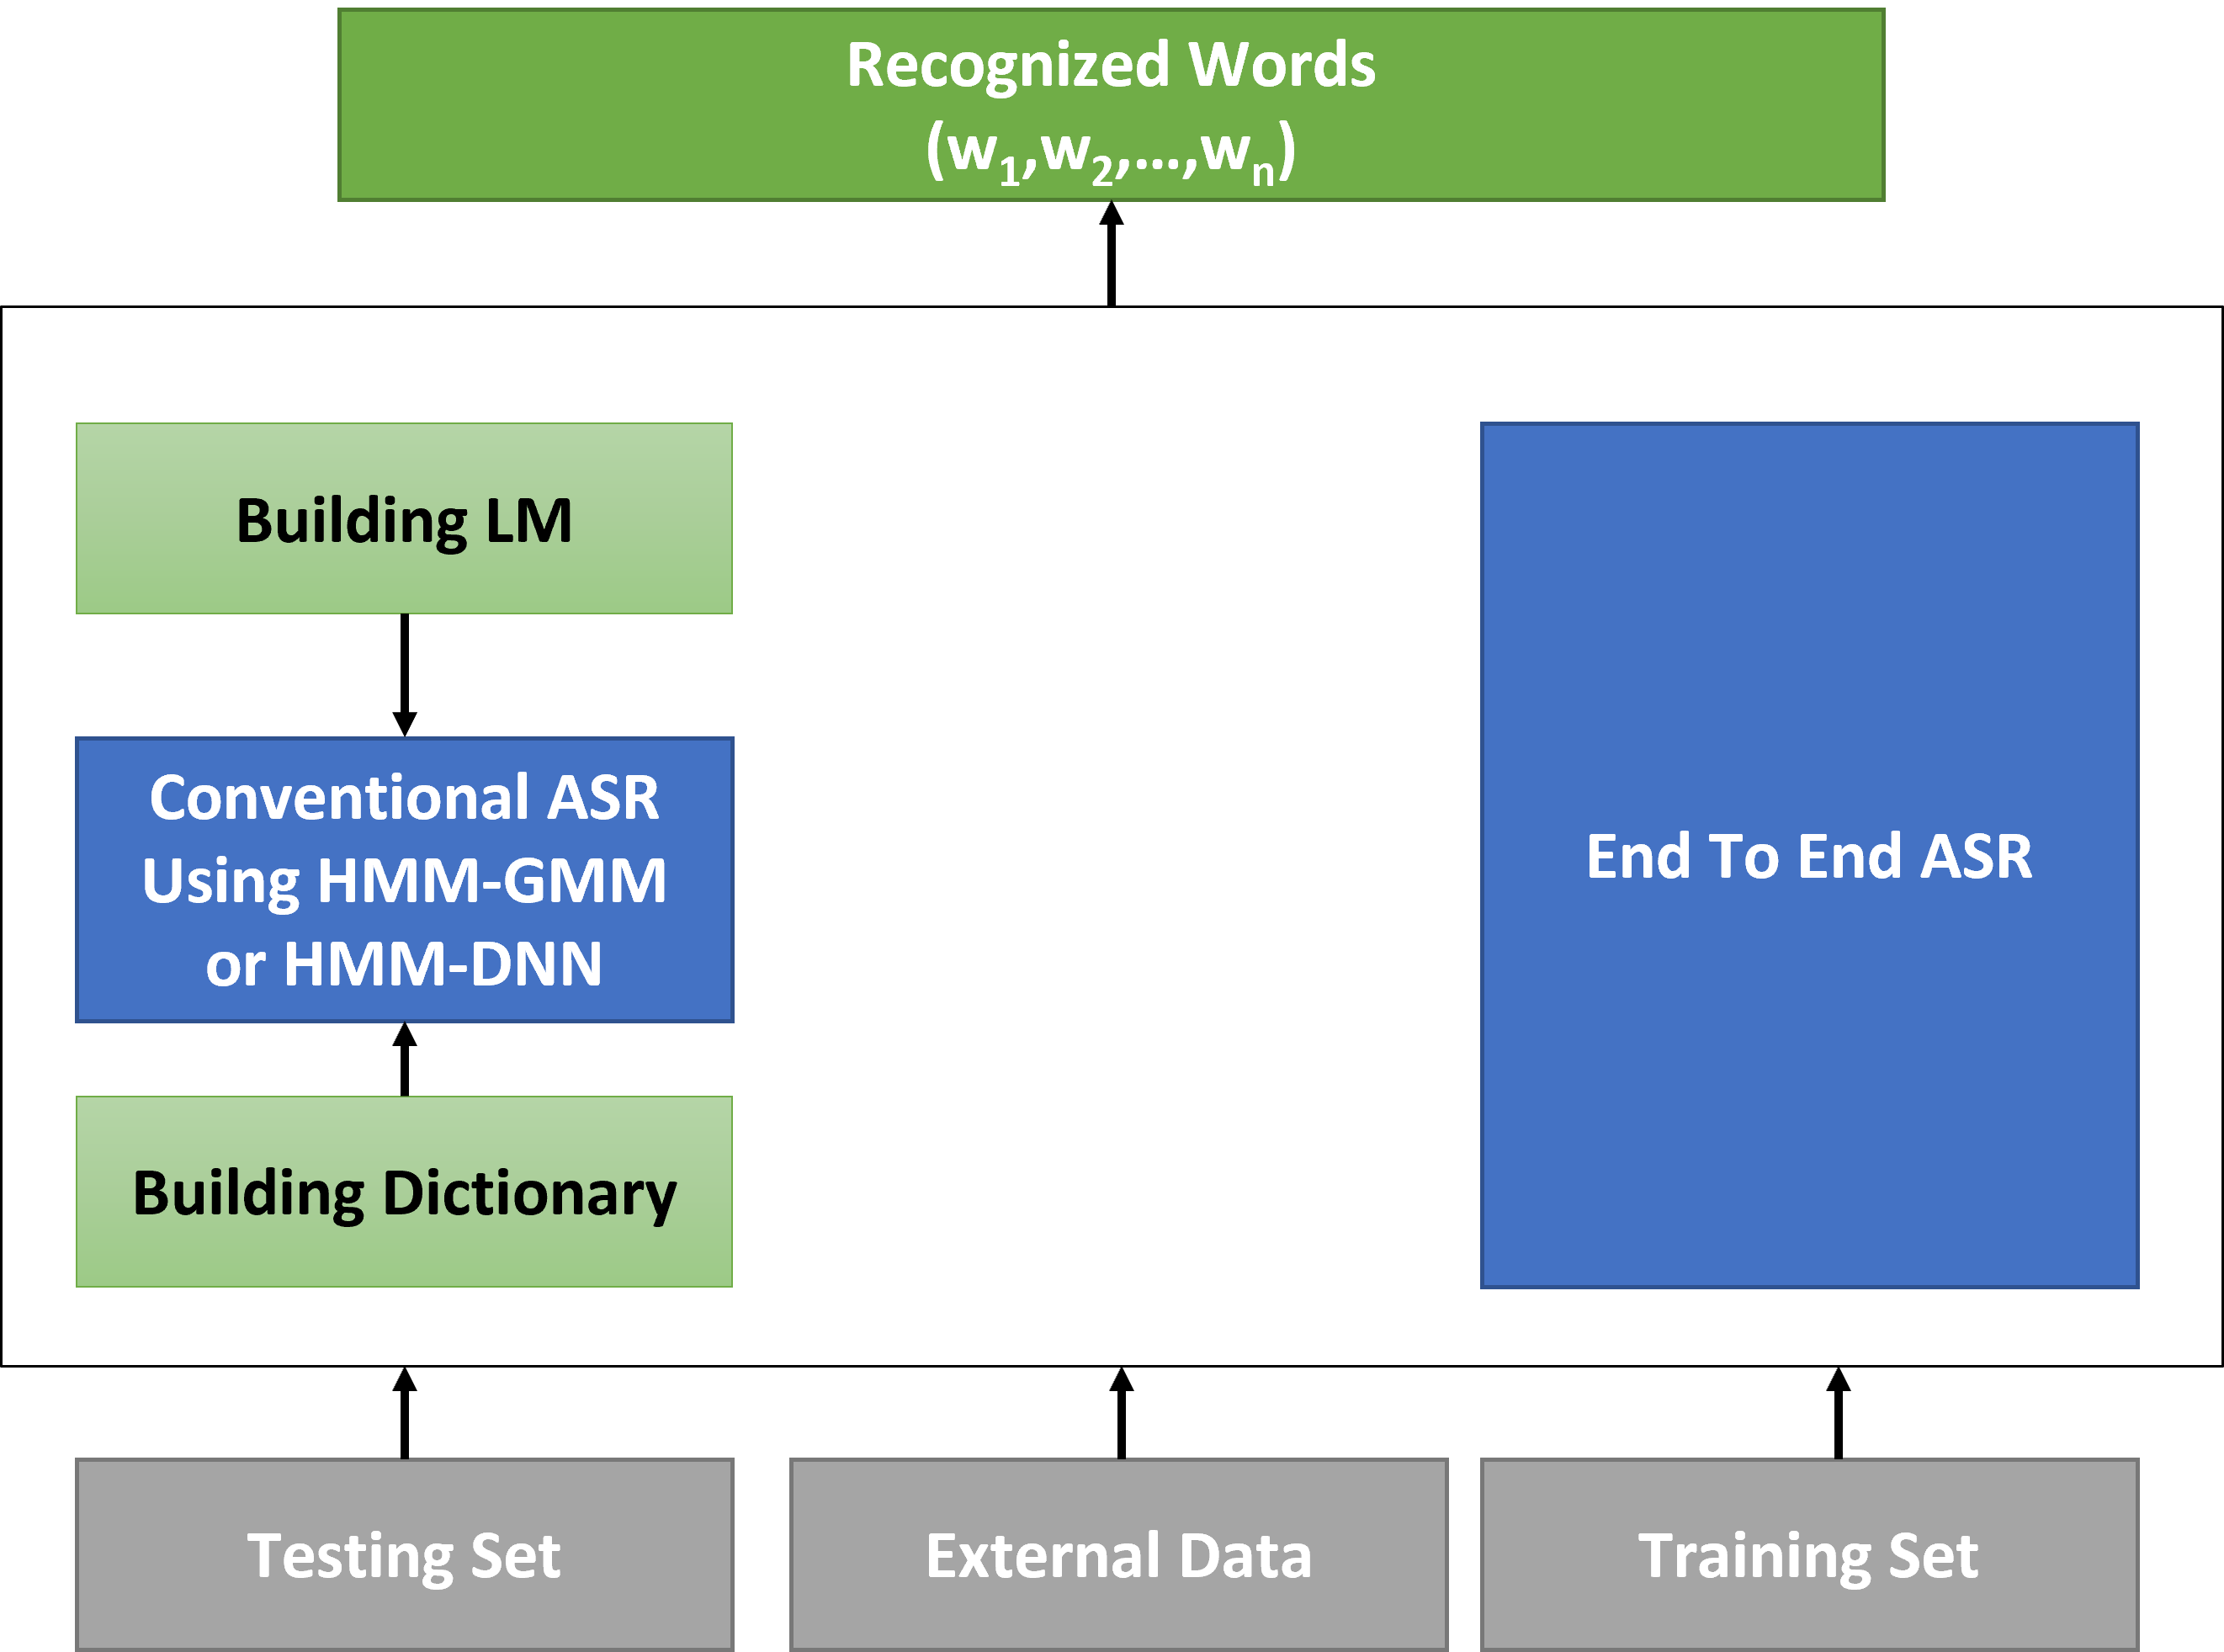
\includegraphics[width=0.6\textwidth]{img/E2EvsConventional.png}
    \caption{E2E ASR Architecture vs Conventional}
    \label{fig:e2e-asr}
\end{figure}

The E2E model \cite{eeckt_continual_2021} is a system that directly maps input audio sequence to sequence of words or other graphemes \cite{amodei_deep_2015-1, bell_adaptation_2020} using Deep Neural Networks like RNN \cite{sak_long_2014}, CNN \cite{abdel-hamid_exploring_2013}, TDNN \cite{kreyssig_improved_2018} and CNN-TDNN \cite{ghahremani_acoustic_2016}.

\begin{figure}[h]
    \centering
    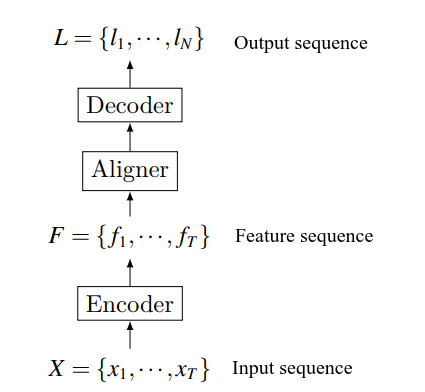
\includegraphics[width=0.4\textwidth]{img/E2E.png}
    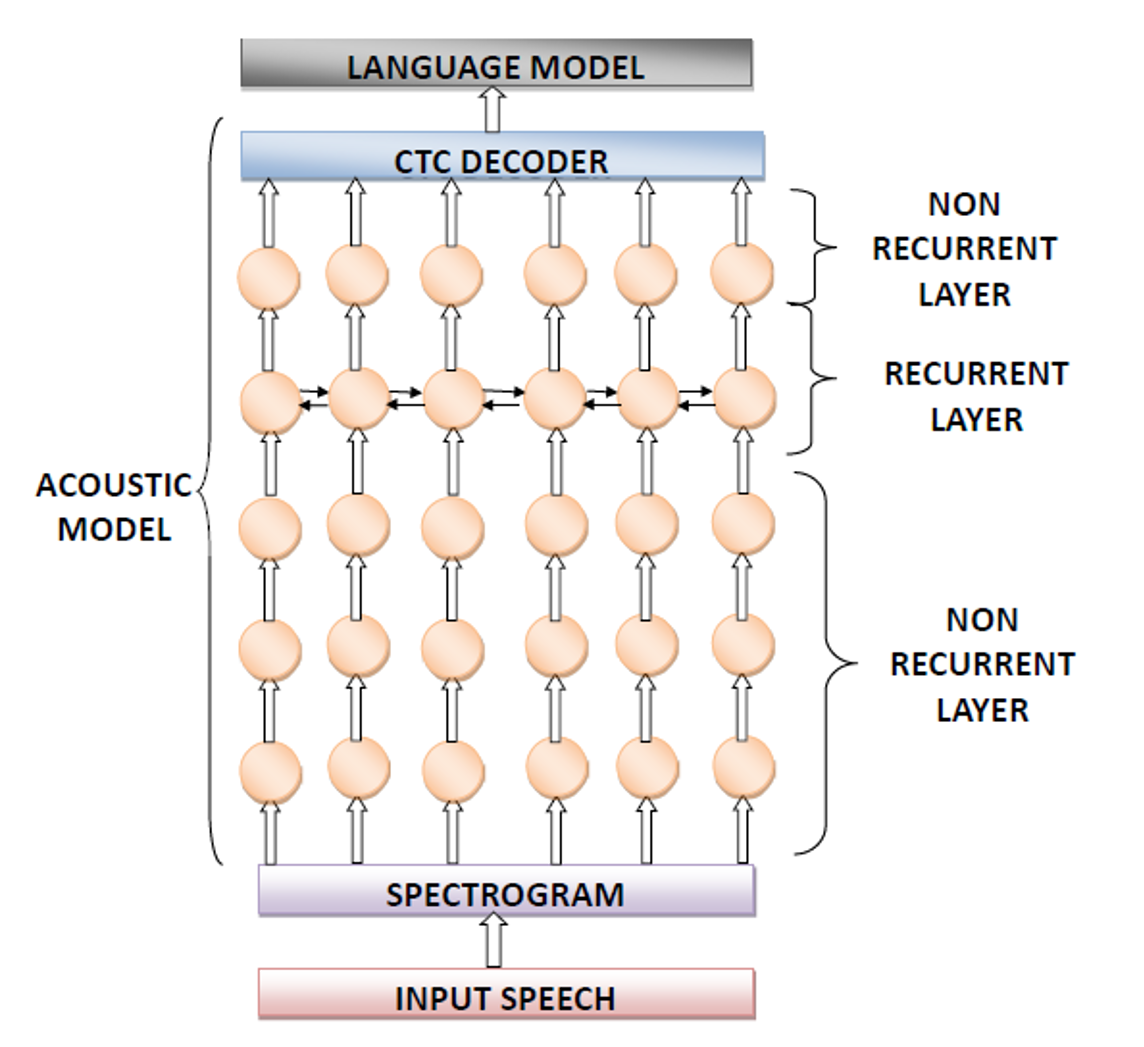
\includegraphics[width=0.4\textwidth]{img/e2est.png}
    \caption{End to End Model}
    \label{fig:e2e-model}
\end{figure}

Despite its triumphs, the use of DNNs in speech processing has the following drawbacks \cite{backstrom_introduction_2022}:

\begin{itemize}
    \item DNN training on a specific dataset does necessarily improve the understanding of the problem. It's a black box because the model's reliability is not known. Although the design process gives some insights about languages, a trained speech recognizer on language "A" does not tell much about speech recognition on language "B" \cite{backstrom_introduction_2022}.
    \item DNN training is highly dependent on the data used to train it e.g. Models can be vulnerable to hidden biases, resulting in poor performance for OOVs or in a different scenario \cite{zhang_strategies_2019}.
    \item A trained DNN solves a specific problem, but does not tell how good the solution is. If a data set represents a circle in the 2D plane, that dataset can be accurately modelled with Sigmoids as non-linearities with a neural network. The neural network only needs to be large enough to handle the task at hand. The network, on the other hand, is several orders of magnitude more complex than the circle equation, which means that even though the network was successfully trained and the model is reasonably accurate, it gives no indication of whether the network's complexity is comparable to the problem's complexity \cite{backstrom_introduction_2022}.
    \item E2E models that are primarily DNN based typically require a large amount of training dataset, 1000 to 100,000 hours of speech to achieve peak performance. Such information is rarely available while also necessitating the purchase of costly hardware and computational resources \cite{kincaid_state_2018}.
    
\end{itemize}

To tackle these issues, the recent model design trend has been to return to classical design paradigms, in which models are based on a in-depth understanding of the problem, particularly in the case of Low-Resource Languages and the parameters of those models are then trained using ML methods \cite{backstrom_introduction_2022}.   

\section{Training ASRs using Statistical Methods with Neural Networks}

Different modules in the HMM-based model employ various technologies and serve different roles. HMM is primarily used at the frame level to perform dynamic time warping, while GMM and DNN are used to compute the emission probability of HMM hidden states \cite{georgescu_kaldi-based_2019}. The HMM-GMM model served as the foundation for many speech recognition systems, but with advancement in deep learning technology DNN was used to calculate the posterior probability of the HMM state instead of the traditional GMM observation-probability. DNN is now used for language and acoustic modelling instead of HMM-GMM model because HMM-DNN outperforms HMM-GMM in terms or accuracy. \cite{dahl_context-dependent_2012}. %and thus becomes the state-of-the-art ASR model.

\begin{figure}[h]
    \centering
    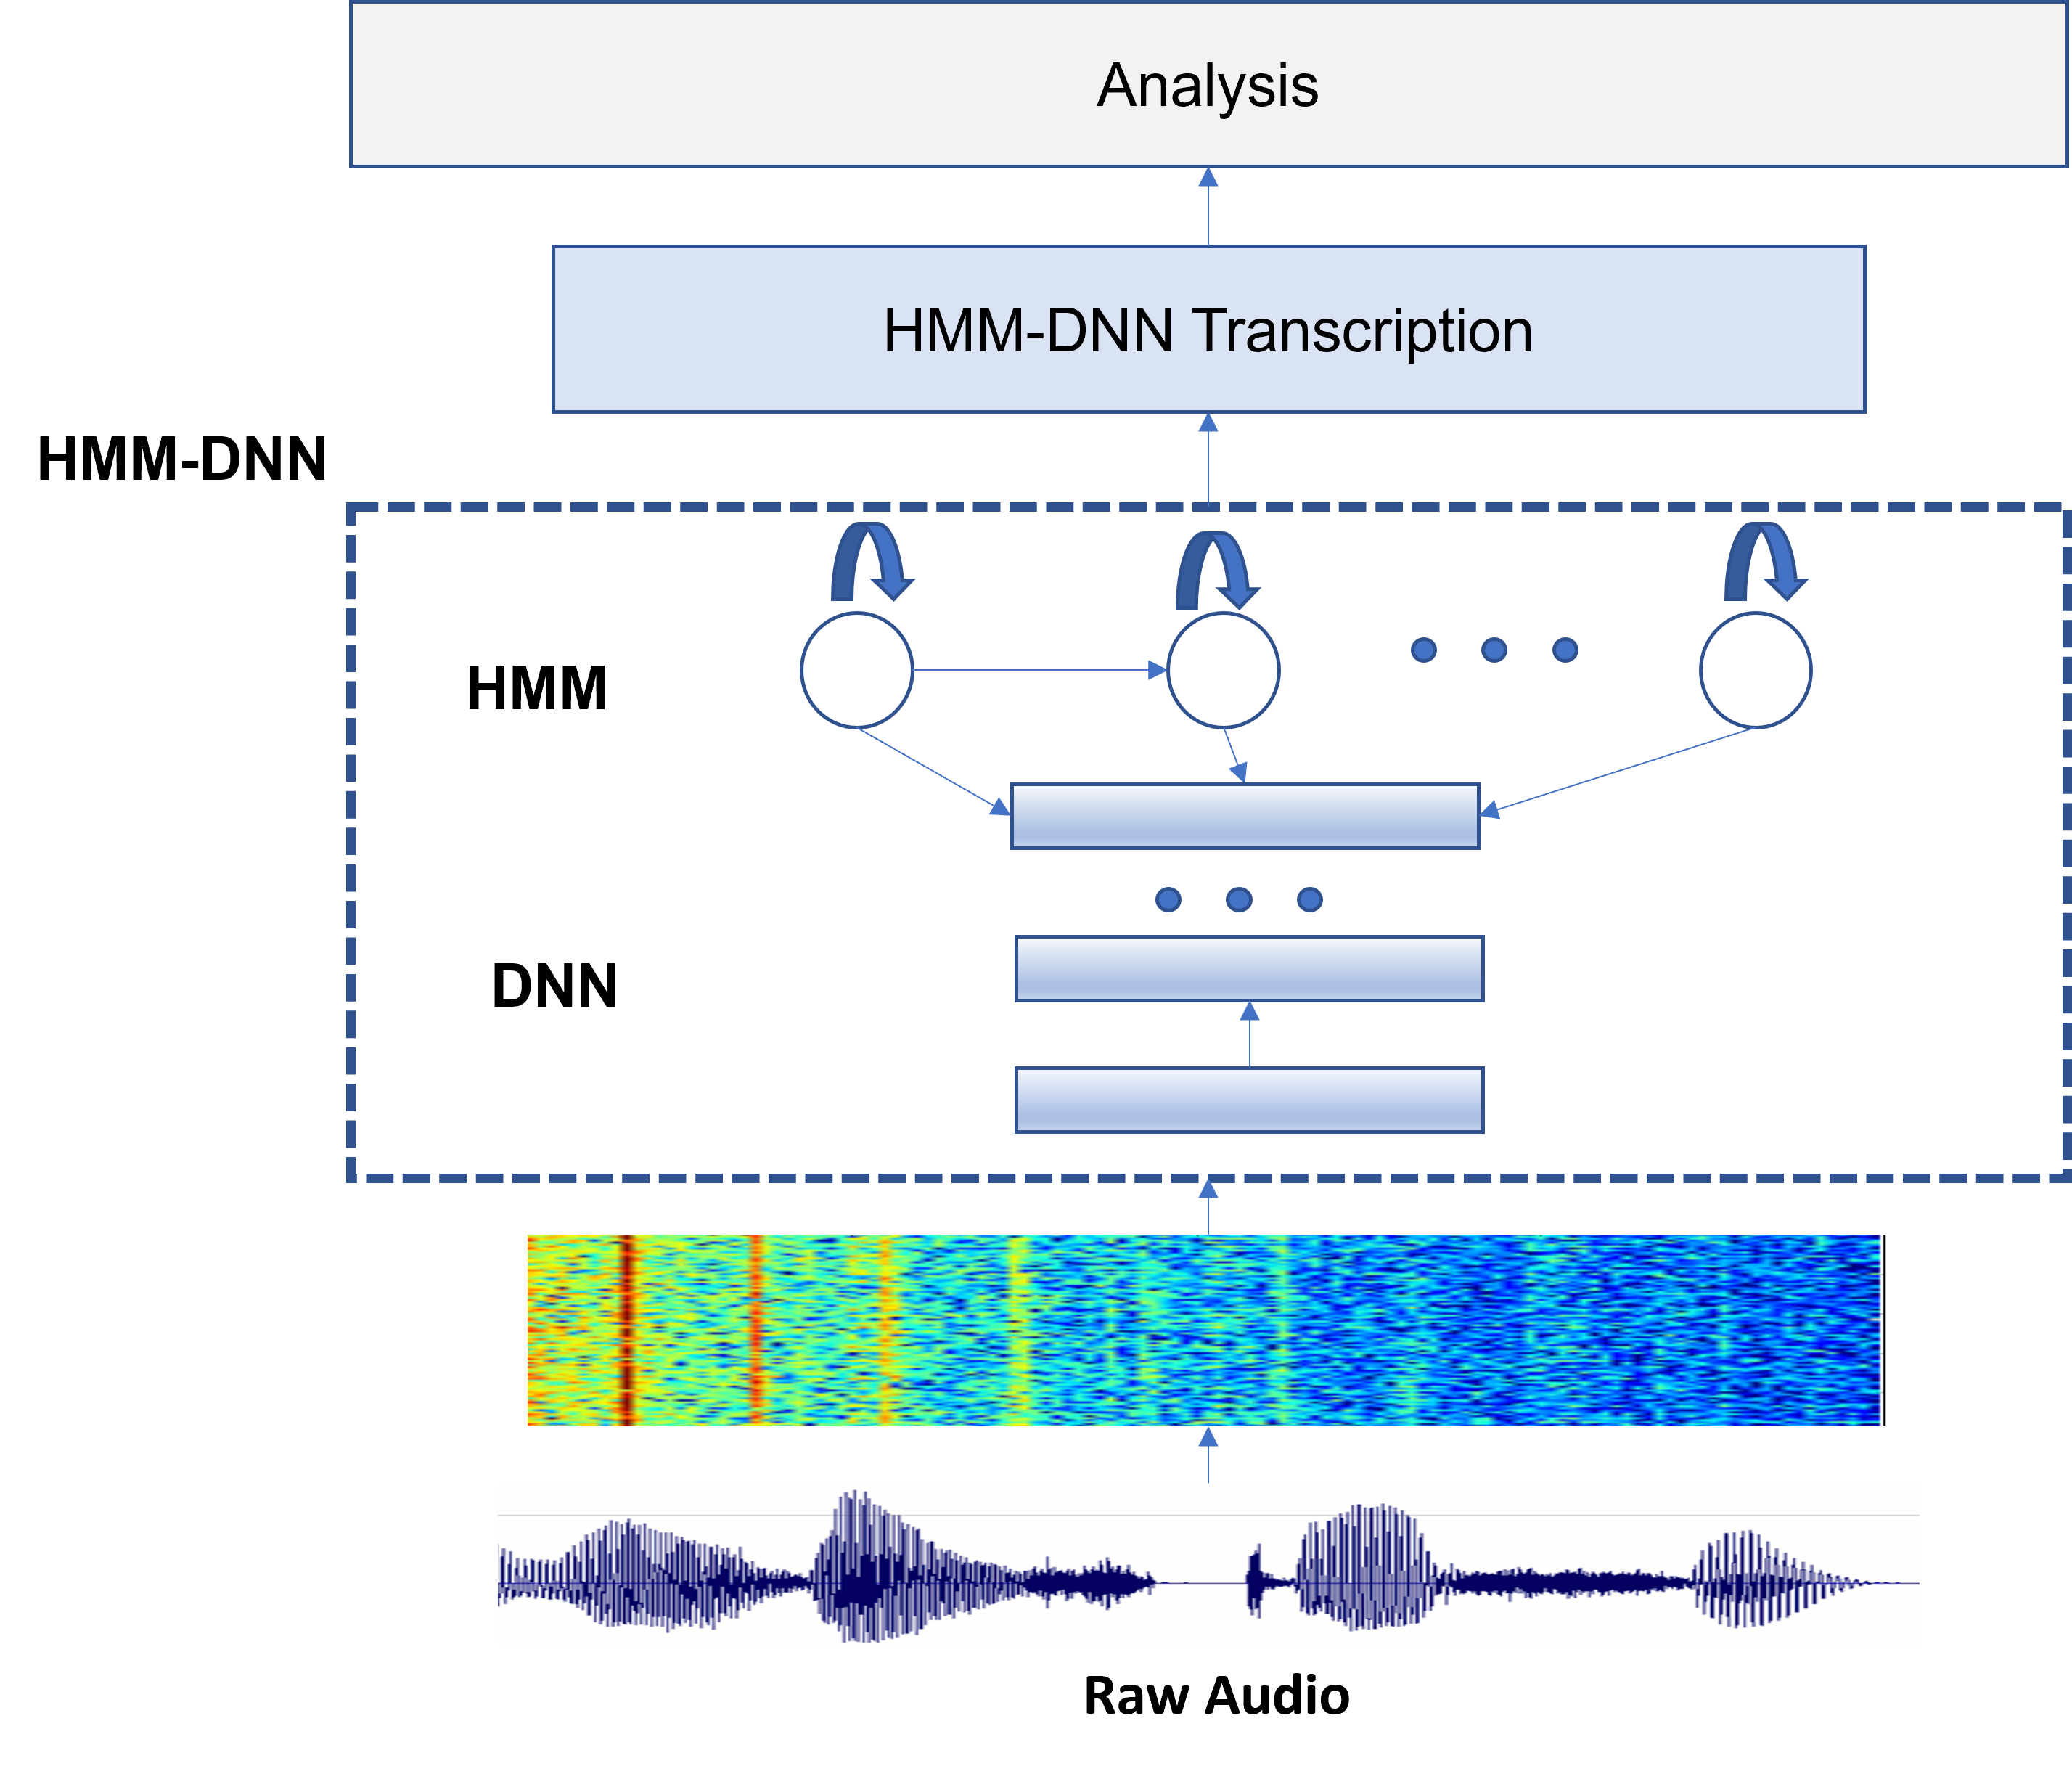
\includegraphics[width=0.5\textwidth]{img/HMM-DNN.png}
    \caption{HMM-DNN Architecture}
    \label{fig:Hmm-dnn-arch}
\end{figure}

One of the first application of HMM–DNN hybrid approach was by Dahl Et al 2012 \cite{dahl_context-dependent_2012} in which Deep neural network model replaced GMM which increased accuracy compared to traditional HMM-GMM legacy system in LVCSR. Many DNN architectures were explored for the acoustic modeling, including Recurrent Neural Networks (RNNs), Bidirectional RNNs (BDRNNs), and deep conditional random fields \cite{graves_speech_2013, hifny_unified_2015}. \cite{vijayaditya_time_2015} proposed a time delay neural network (TDNN) which gave improved results in learning wider temporal dependencies in comparison to models based on DNN or RNN. 

Various studies \cite{smit_advances_2021, li_hybrid_2013, ochiai_speaker_2016} modeled the acoustic component of ASR system using Deep Neural Networks, referred to as Hybrid DNN-HMM approach. Rectified Linear Units (ReLU) and maxout units are commonly used in ASR systems as activation functions to model non-linearity in DNN \cite{backstrom_introduction_2022}. 

\begin{figure}[h]
    \centering
    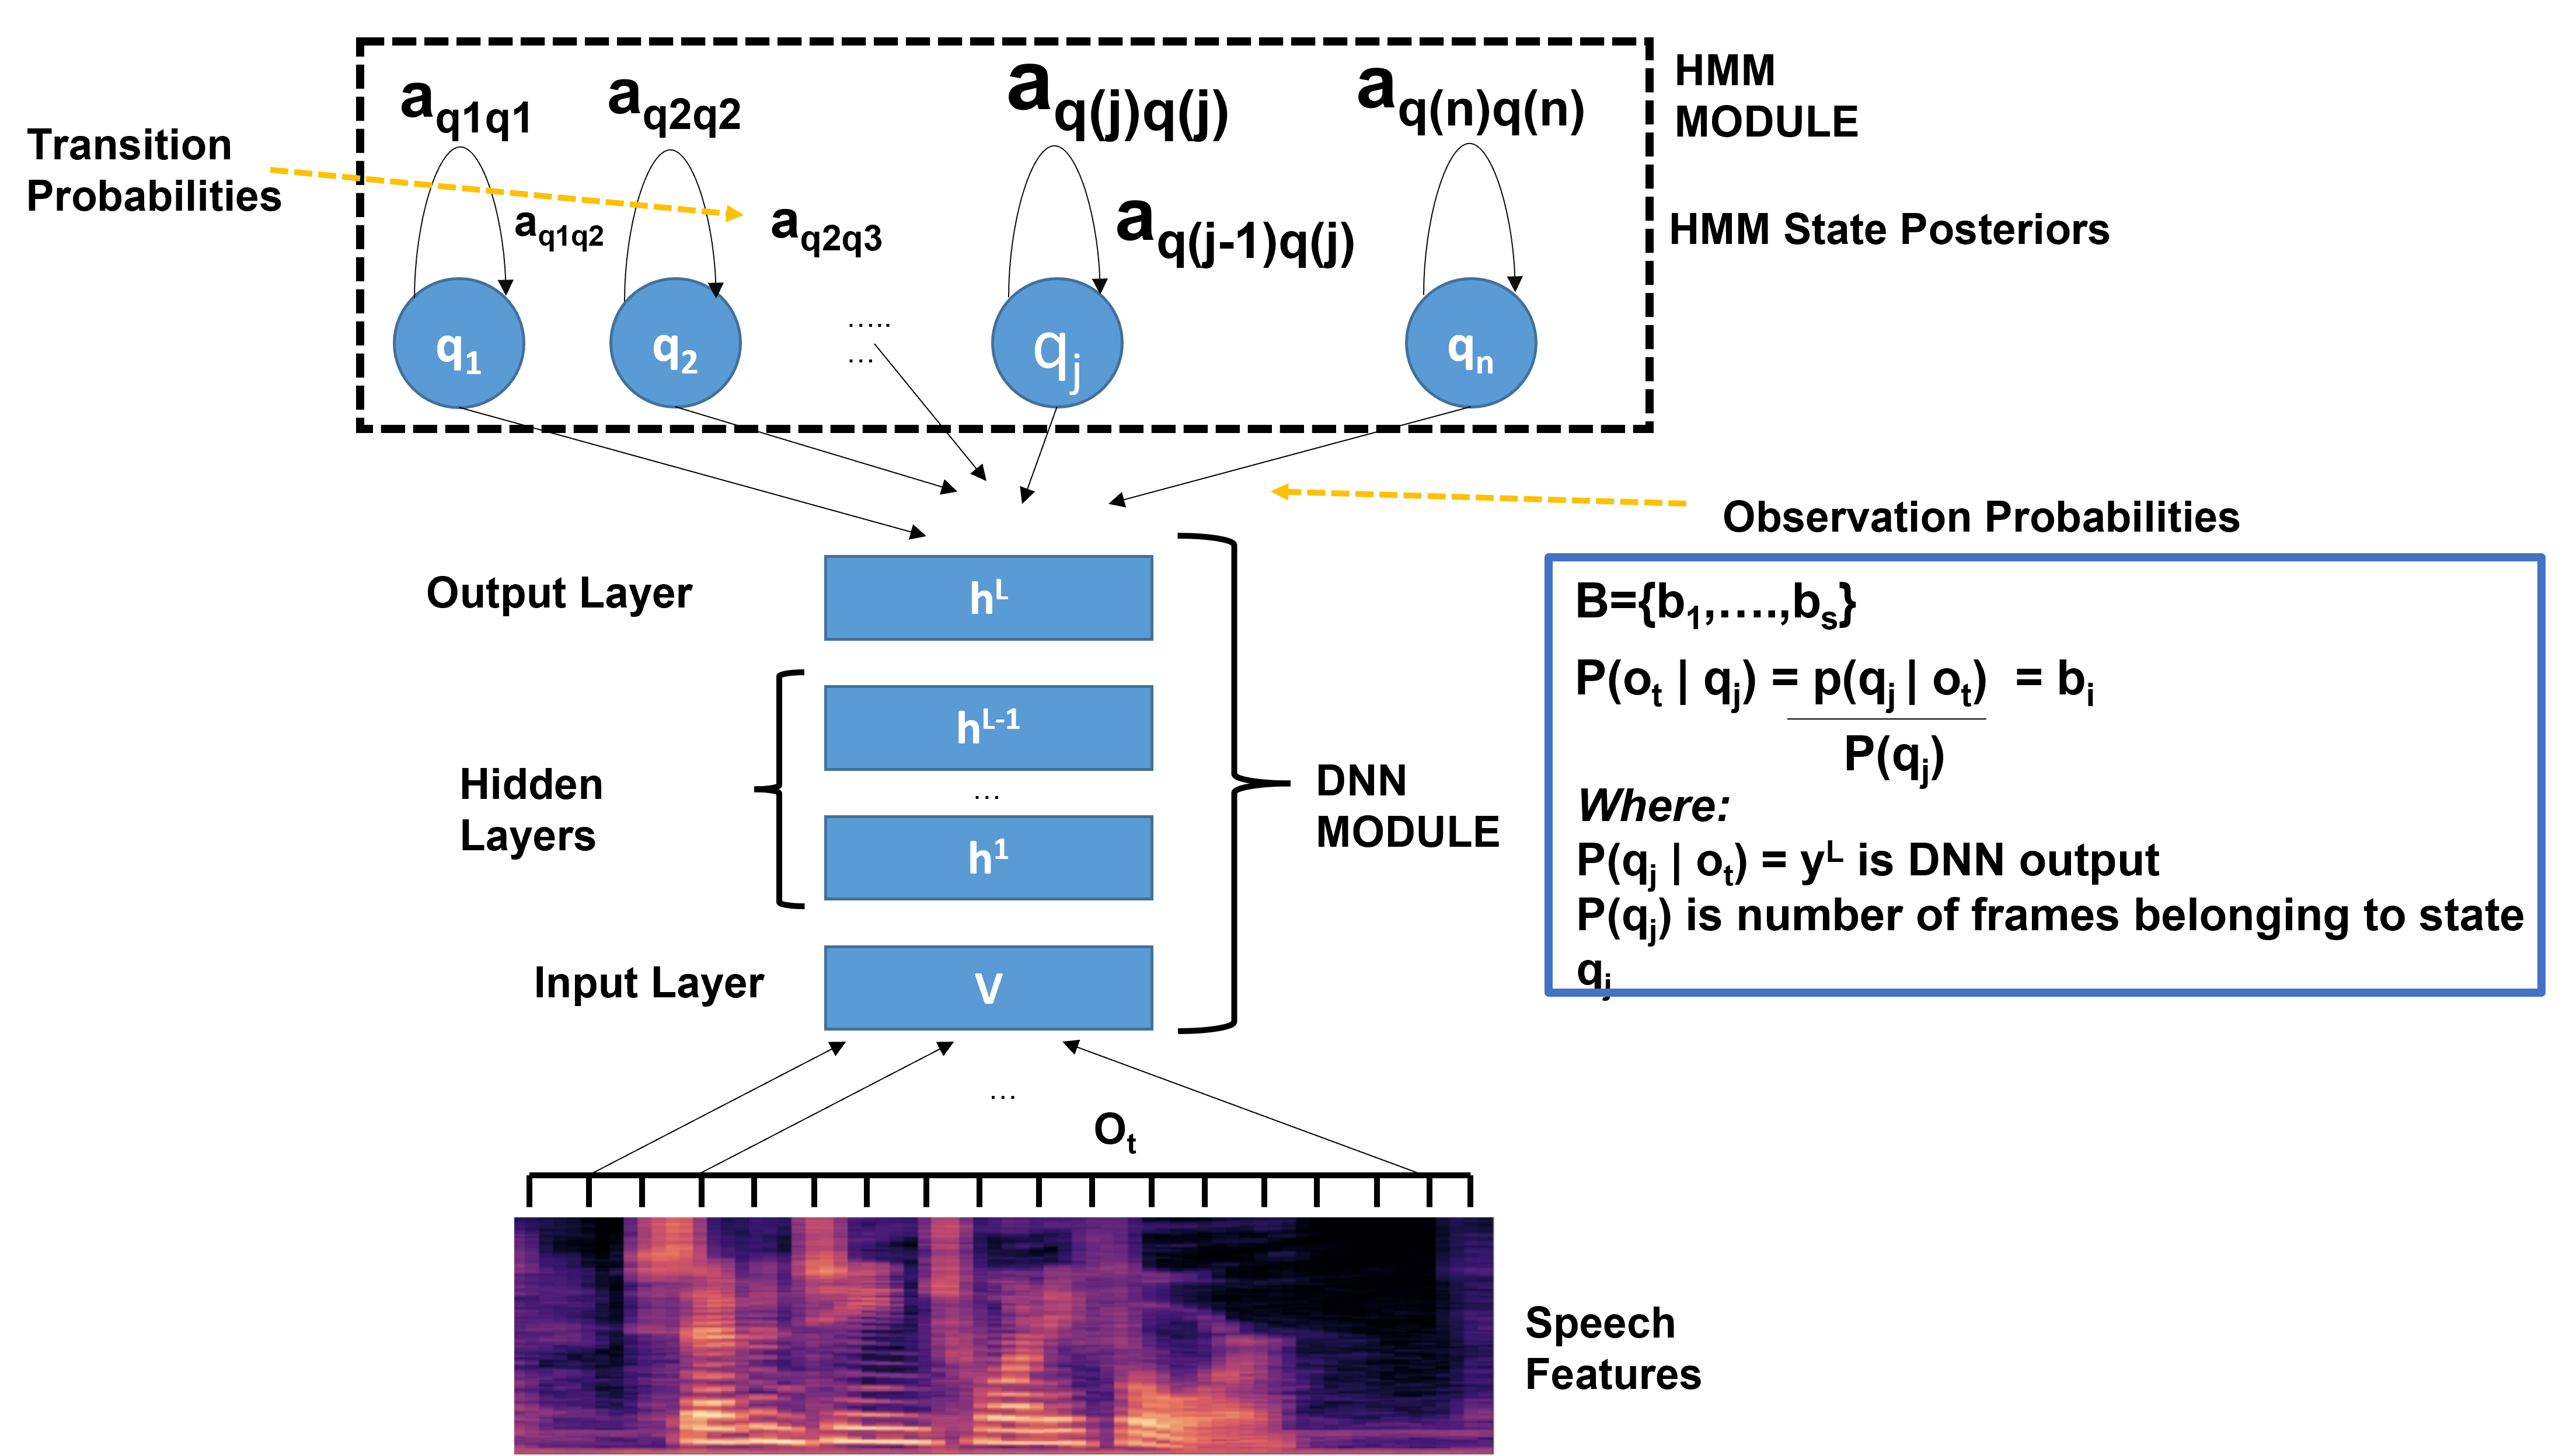
\includegraphics[width=0.95\textwidth]{img/generic-Hmm-DNN.png}
    \caption{Working of HMM-DNN ASR}
    \label{fig:working-hmm-dnn}
\end{figure}

In HMM DNN System audio is broken into segments and frames and features are taken as input in the input layer. This input is passed via Hidden layers into output Layer on which we apply HMM state posteriors attained from observation and Transition Probabilities. DNN models the scaled observation likelihood of all senones or tied Triphone states, while HMM models the sequential property of speech signals. The same DNN is replicated at various points in time \cite{hussein_arabic_2022}.

Hidden units complicate training weights because each hidden unit indirectly affects the error function via all output units. Credit assignment problem 
involves determining hidden unit error and the importance of the input-hidden weight to the output unit which is solved by back-propagating gradients through the network - the gradient for a hidden unit output with respect to error can be calculated as the weighted sum of the deltas of the connected output units (Propagate the values backwards through the network). The back-propagation of error or back-prop algorithm allows the propagation of error gradients through a deep network in order to perform gradient descent training \cite{dahl_context-dependent_2012}.

%\begin{figure}[h!]
%    \centering
%    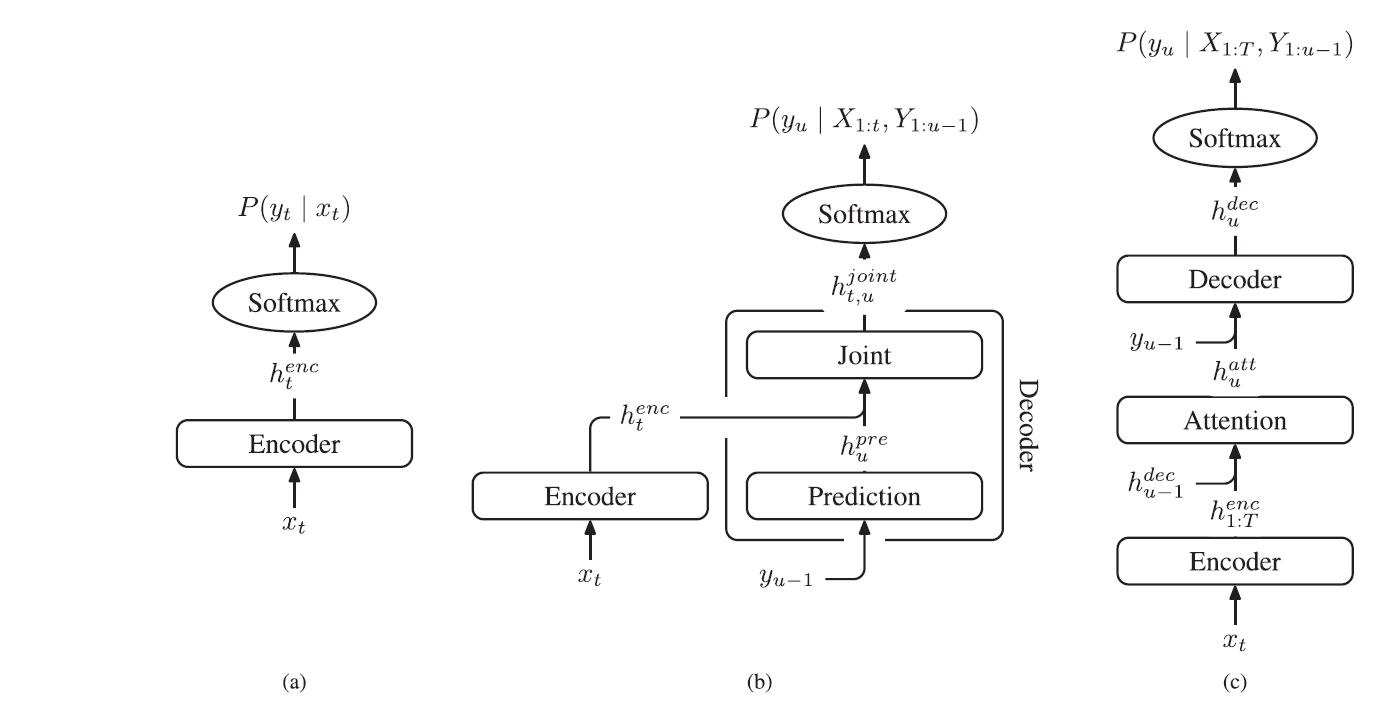
\includegraphics[width=0.9\textwidth]{img/hybridande2e.png}
%    \caption{NN architectures for Hybrid NN/HMM and E2E}
%    \label{fig:hybrid-e2e}
%\end{figure}

%Figure \ref{fig:hybrid-e2e} shows NN architectures used for hybrid NN/HMM and end-to-end (CTC, RNN-T, AED) speech recognition systems:
%\begin{enumerate}[label=(\alph*)]
%    \item Scheme of NN in NN/HMM hybrid systems and CTC
%    \item RNN Transducer (RNN-T) architecture
%    \item Attention based encoder-decoder (AED) end-to-end systems architecture in which $x_{t}$ denotes input acoustic feature vectors; $h_{t}$ and $h_{u}$ denotes hidden layers, and $y_{t}$, $y_{u}$ denotes output labels, depends if they are indexed by time \textit{t} in hybrid and CTC systems or only by output label \textit{u} in parts of RNN-T and AED systems. The encoders use a wide temporal context as input, in practice, even the whole acoustic sequence in the case of most CTC and AED models.
%\end{enumerate}

%\subsection{Context Dependent Hybrid HMM-DNN}
Context-dependent HMM/GMM system is trained on the same data for a Context-Dependent Hybrid HMM-DNN, using a phonetic decision tree to determine the HMM tied states. Then, using the trained HMM/GMM and the training data, Viterbi alignment is performed after which a neural network is trained to map the input speech features to a label representing a context-dependent tied HMM states \cite{dahl_context-dependent_2012}. 

\begin{figure}[h]
    \centering
    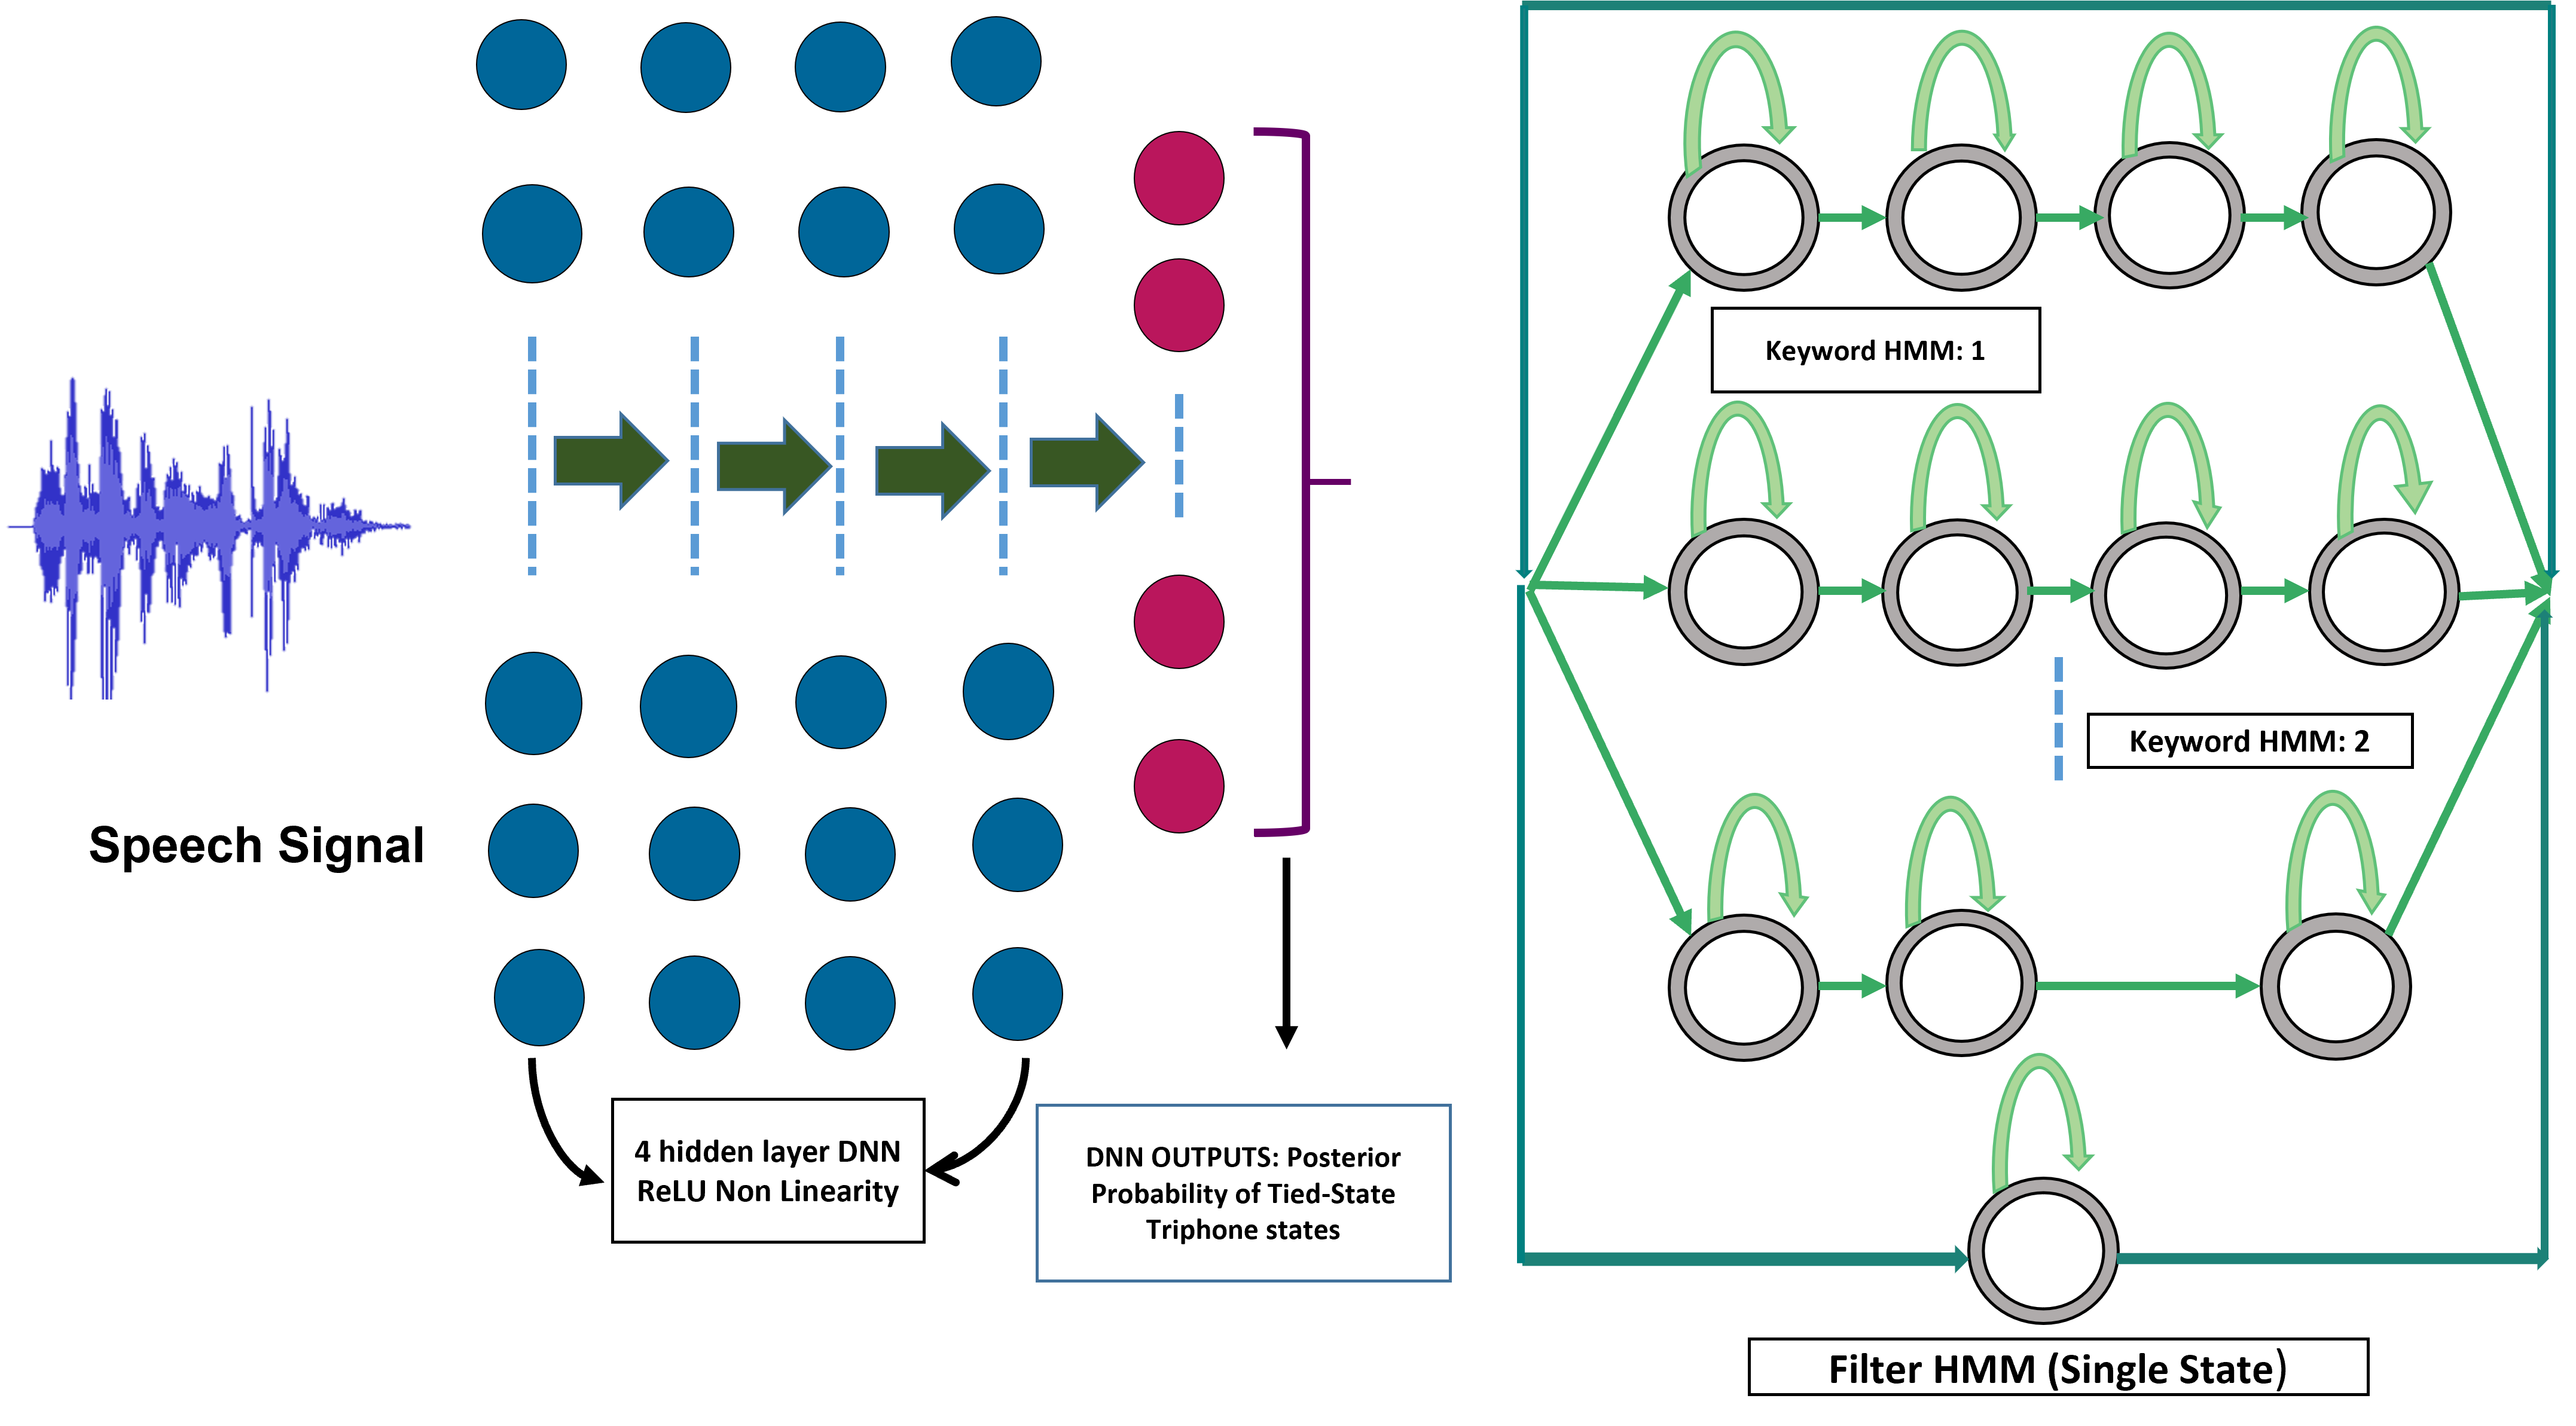
\includegraphics[width=0.95\textwidth]{img/CDHMMDNN.png}
    \caption{Context Dependent HMM-DNN}
    \label{fig:CDHMMDNN}
\end{figure}

The label set is thousands (number of context-dependent tied states) rather than tens of thousands (number of context-independent phones). The Viterbi aligned tied state is then assigned to each frame. Using gradient descent as usual we  train the neural network and decode using the neural network's context-dependent scaled likelihoods \cite{seide_feature_2011}.

\subsection{Benefits of combining HMM and Neural Networks}

Advantages of using HMM-DNN models include:
\begin{itemize}
     \item It is a practical and effective method for ASR deployment on Low Computational Resources compared to Deep Learning Methods. 
     \item It takes less time to train in contrast to Deep Learning Methods \cite{naeem_subspace_2020}.
    \item Maintains the Structure that is required for a Language and Speech Processing System based on which the computer can understand the language better \cite{kincaid_state_2018}. Hence this works better in an environment where the context of speech is of the essence and has been applied for Continuous Speech Recognition as well \cite{backstrom_introduction_2022, morgan_continuous_1995}. 
    \item DNN-HMM can extend the labelling ability of GMM-HMM when the hidden layer and hidden unit numbers are set up properly in comparison to GMM-HMMs, shallow-NN-HMMs, and Multi-layer Perceptrons HMMs (MLPHMMs). Thus, DNN-HMMs with discriminative pre-training can produce good results in our scenario as well \cite{li_hybrid_2013}.
    \item HMM–DNN (especially TDNN) is streamable while E2E-transformer is not \cite{ritter_neural_2019}. 
    \item Computationally intensive compared to E2E Systems \cite{kincaid_brief_2018}.
    \item E2E modelling is less mature than hybrid modelling, and much of the research on E2E modelling is focused on improving general modelling technology \cite{backstrom_introduction_2022}. 
    \item Easily models correlated features like spectral features and input context includes multiple data-frames at input \cite{backstrom_introduction_2022}. 
    \item Because E2E models typically contain sub-networks corresponding to the acoustic model and language model in hybrid models, most adaptation technologies successfully applied to hybrid models by adapting acoustic model or language model can also work well for E2E models \cite{backstrom_introduction_2022}. %Most adaptation technologies successfully applied to hybrid models by adapting acoustic model or language model can also work well for E2E models \cite{backstrom_introduction_2022} since E2E models typically contain sub-networks corresponding to the acoustic model and language model in hybrid models.
    \item Greater flexibility than GMMs because it is not made of nearly local components since GMMs are inefficient for non-linear class boundaries \cite{bell_adaptation_2021}.
    \item NNs can simultaneously model multiple events in the input compared to GMMs, i.e. different sets of hidden units modelling each event, whereas GMMs assume generation of each from by a single mixture component \cite{hussein_arabic_2022}.
    \item NNs can learn more complex representations compared to GMMs and higher-level features such as tandem, posteriorgrams, bottleneck features (like in TDNN) etc \cite{liu_time_2019}.
    \item Components in hybrid HMM-DNN models are optimised separately, whereas E2E models use a single objective function which is why E2E models tend to memorise the training data more, making generalisation or robustness to unseen data difficult for E2E models. Thus, adaptation to a new environment or domain is critical to the large-scale application of E2E models \cite{backstrom_introduction_2022}. 
\end{itemize}

However, HMM–DNN models have some drawbacks like model complexity i.e. complicated to implement since it deploys a modular design, separately training different modules for acoustic modeling, pronunciation lexicon, and language modeling,  requiring of linguistic resources \cite{hussein_arabic_2022}. But as a trade-off for performance, data-set and computation requirement, in our scenario, Using HMM-DNN makes the most sense \cite{georgescu_performance_2021}.

\subsection{Using Maximum Mutual Information Model for HMM-DNN Systems}

Discriminative objective functions like Maximum Mutual Information (MMI) or Maximum Conditional Likelihood Estimation objective functions are trained to maximize the gap between the correct and incorrect answers, or to differentiate between right and wrong answers instead of assigning high weights values to the correct sequences which helps training model to improve the correct output sequence prediction, while making incorrect sequences less likely \cite{povey_purely_2016}. 

Deep networks excel in feature extraction and discovering correlation among them which allows exploitation of contents in making predictions. DNN can be used in ASR to classify phones based on the features extracted in acoustic frames. It is treated like a classifier using softmax to output the probability distribution $P(phone | x_{i})$. The softmax pulls up the ground truth while pulls down the others which is the same concept as Maximum Mutual Information Estimation \cite{wiesner_lattice_2020}.

\begin{equation}
 p_{i} = \frac{e^{score_{i}}}{\sum_{c \in y} e^{score_c}}
\end{equation}

Maximum Likelihood Estimation uses sequence training but it is not discriminative. The softmax function is discriminative here. The term Sequence means that the objective considers the entire utterance rather than "frame-level" objectives such as cross-entropy. The term discriminative refers to the use of an objective function that supposedly optimises some task-related criteria, and then directly minimising that objective using gradient-based methods \cite{noauthor_lattice_nodate}.

To turn MLE into a discriminative sequence training, the classifier is trained by minimizing the cross-entropy and the model is utilized to generate alignments and lattices which is called the discriminative training phase. 

The second phase is the sequence training. Since both the deep network and the lattice are network objects, they can be trained together. This model is then used to calculate the MMIE or Minimum Phone Error objective with the forward-backward algorithm followed by back-propagation to learn the model parameter \cite{wiesner_lattice_2020}.

MMI objective for ASR can be expressed as \cite{noauthor_lattice_nodate}:
\begin{equation}
    F_{MMI}(\theta) = \sum_{r=1}^{R} log \frac{P_{\theta}((O_{r}|M_{Wr})P(w_{r})}{\sum_{\hat{w}}P_{\theta}(O_{r}|M_{\hat{w}})P(\hat{w})} 
\end{equation}

Where $M_{w}$ is HMM that corresponds to transcription \textit{w}. To normalise the numerator, the objective function accounts for the log-probability of complete utterance in the numerator dividing it by the log probability of all possible utterances in the denominator. Thus, the distributions with the subscript $\theta$ are trained parameterized distributions \cite{wiesner_lattice_2020}.

%\begin{figure}[h]
%    \centering
%    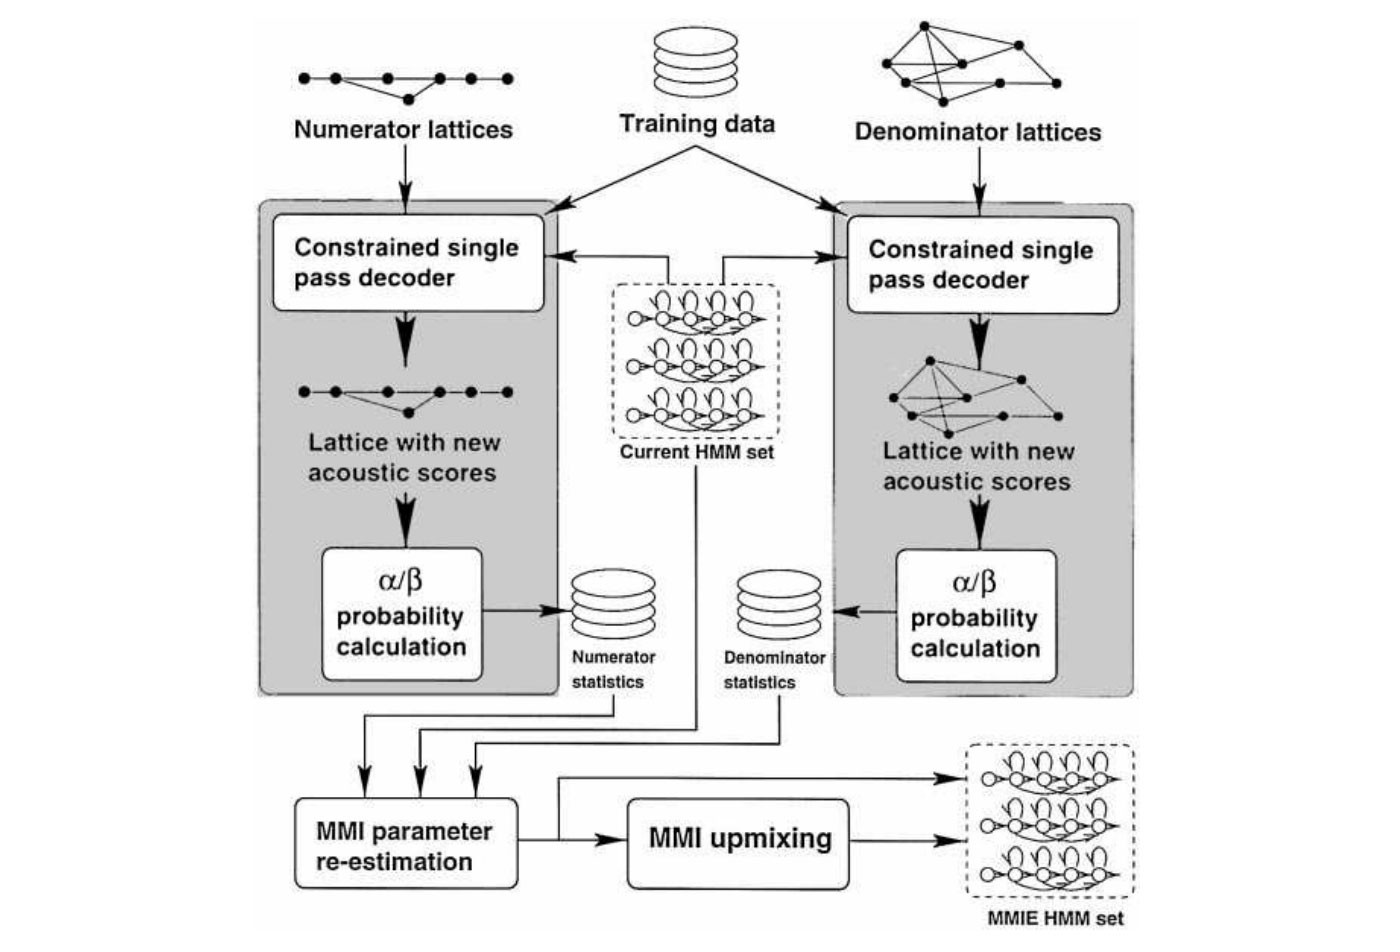
\includegraphics[width=0.9\textwidth]{img/LatticsbasedMMI.jpeg}
%    \caption{Lattice Based MMI system}
%    \label{fig:latt-based-mmi-sys}
%\end{figure}

MMI requires First order Gradient based methods for optimization, such as Stochastic Gradient descent, which requires knowledge of the gradient of the MMI objective with respect to the parameter $\theta$. The neural network function performs forward propagation, while back-propagation computes the corresponding gradient. The state occupancies for the numerator and denominator terms must be computed for the gradient overall objective \cite{daniel_povey_kaldi_nodate}.

Calculating the denominator sum requires summing over an exponentially large amount of word-sequences, which is impractical. Two methods can be used to approximate the sum \cite{noauthor_lattice_nodate}:

\begin{enumerate}
    \item \textbf{N-best list:} This less used and crude method of approximation is computed once and used for all utterances. 
    \item \textbf{Lattice structure:} It can be a word or phone based structure. A path through the lattice denotes a probable phone or word sequence. Lattices require initialization with a trained model which is a drawback, and cross-entropy trained systems are usually used for this purpose. 
\end{enumerate}

%\begin{figure}[h]
%    \centering
%    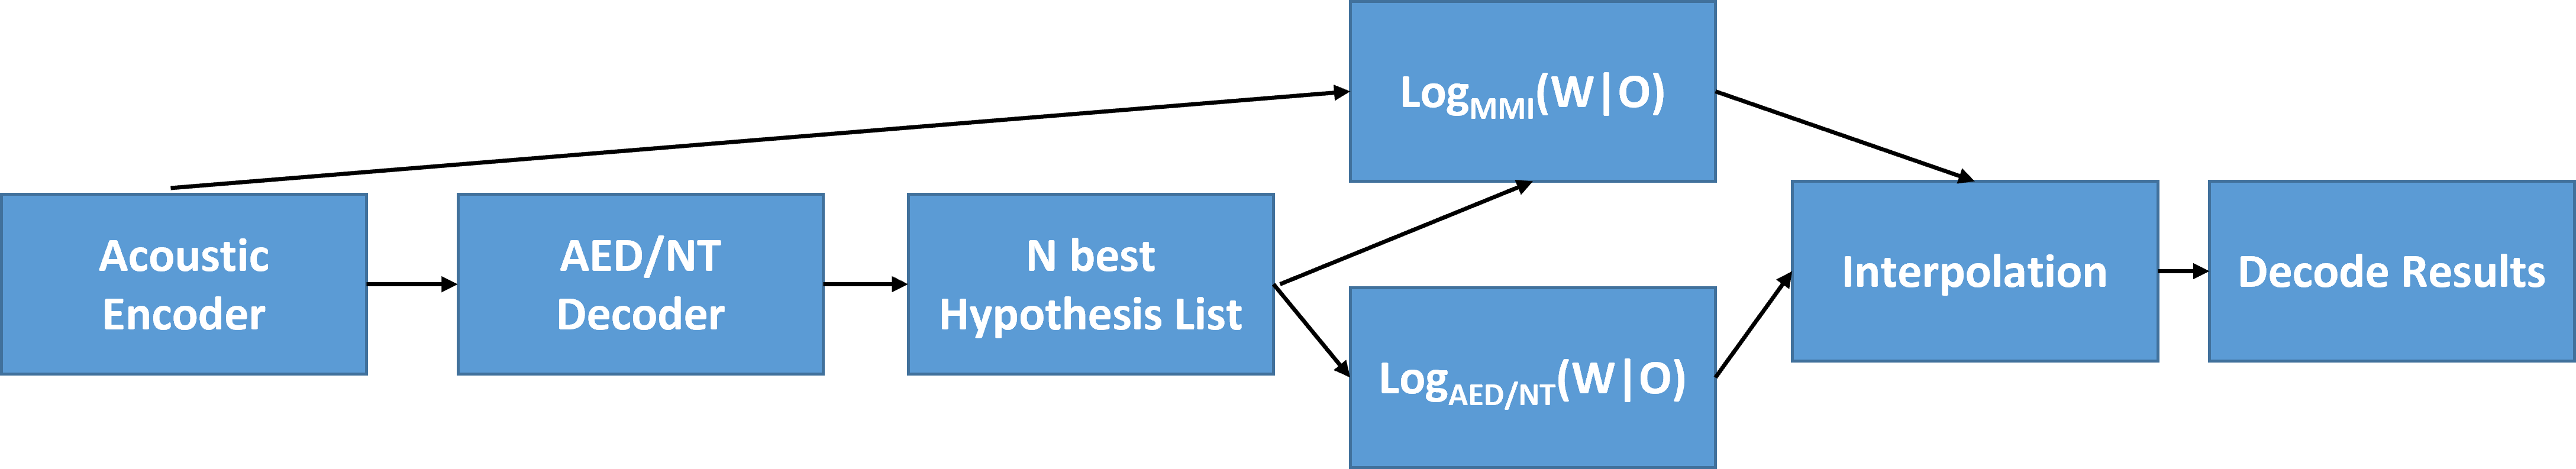
\includegraphics[width=0.9\textwidth]{img/MMISCORING.png}
%    \caption{MMI Scoring}
%    \label{fig:MMI-scoring}
%\end{figure}

The denominator in a lattice-based MMI is first identified by the word lattice. Classifying phones with Deep Learning requires pre-training a deep neural network with cross-entropy. The scaling fudge factor $kappa$ must also be used to correct the overestimation. While training a Deep Neural Network everything seems adhoc but this can be avoided \cite{wiesner_lattice_2020}.

%A composed transducer is generally used in Traditional ASR called H ◦ C ◦ L ◦ G to decode audio. It is a WFST and can be integrated with the deep network classifier. It is a big complex network which can be trained like DNN or DL using back-propagation without the requirement of introduction of a lattice for denominator approximation. Pdf-ids are numerical values of context dependent states given by decoding graphs formed by the decoding algorithms which uses WFSTs to provide graph operations used in acoustic modelling. WFST are used in HMM-GMM models and can also be used along with Deep Neural Network Classifiers.

\begin{figure}[h]
    \centering
    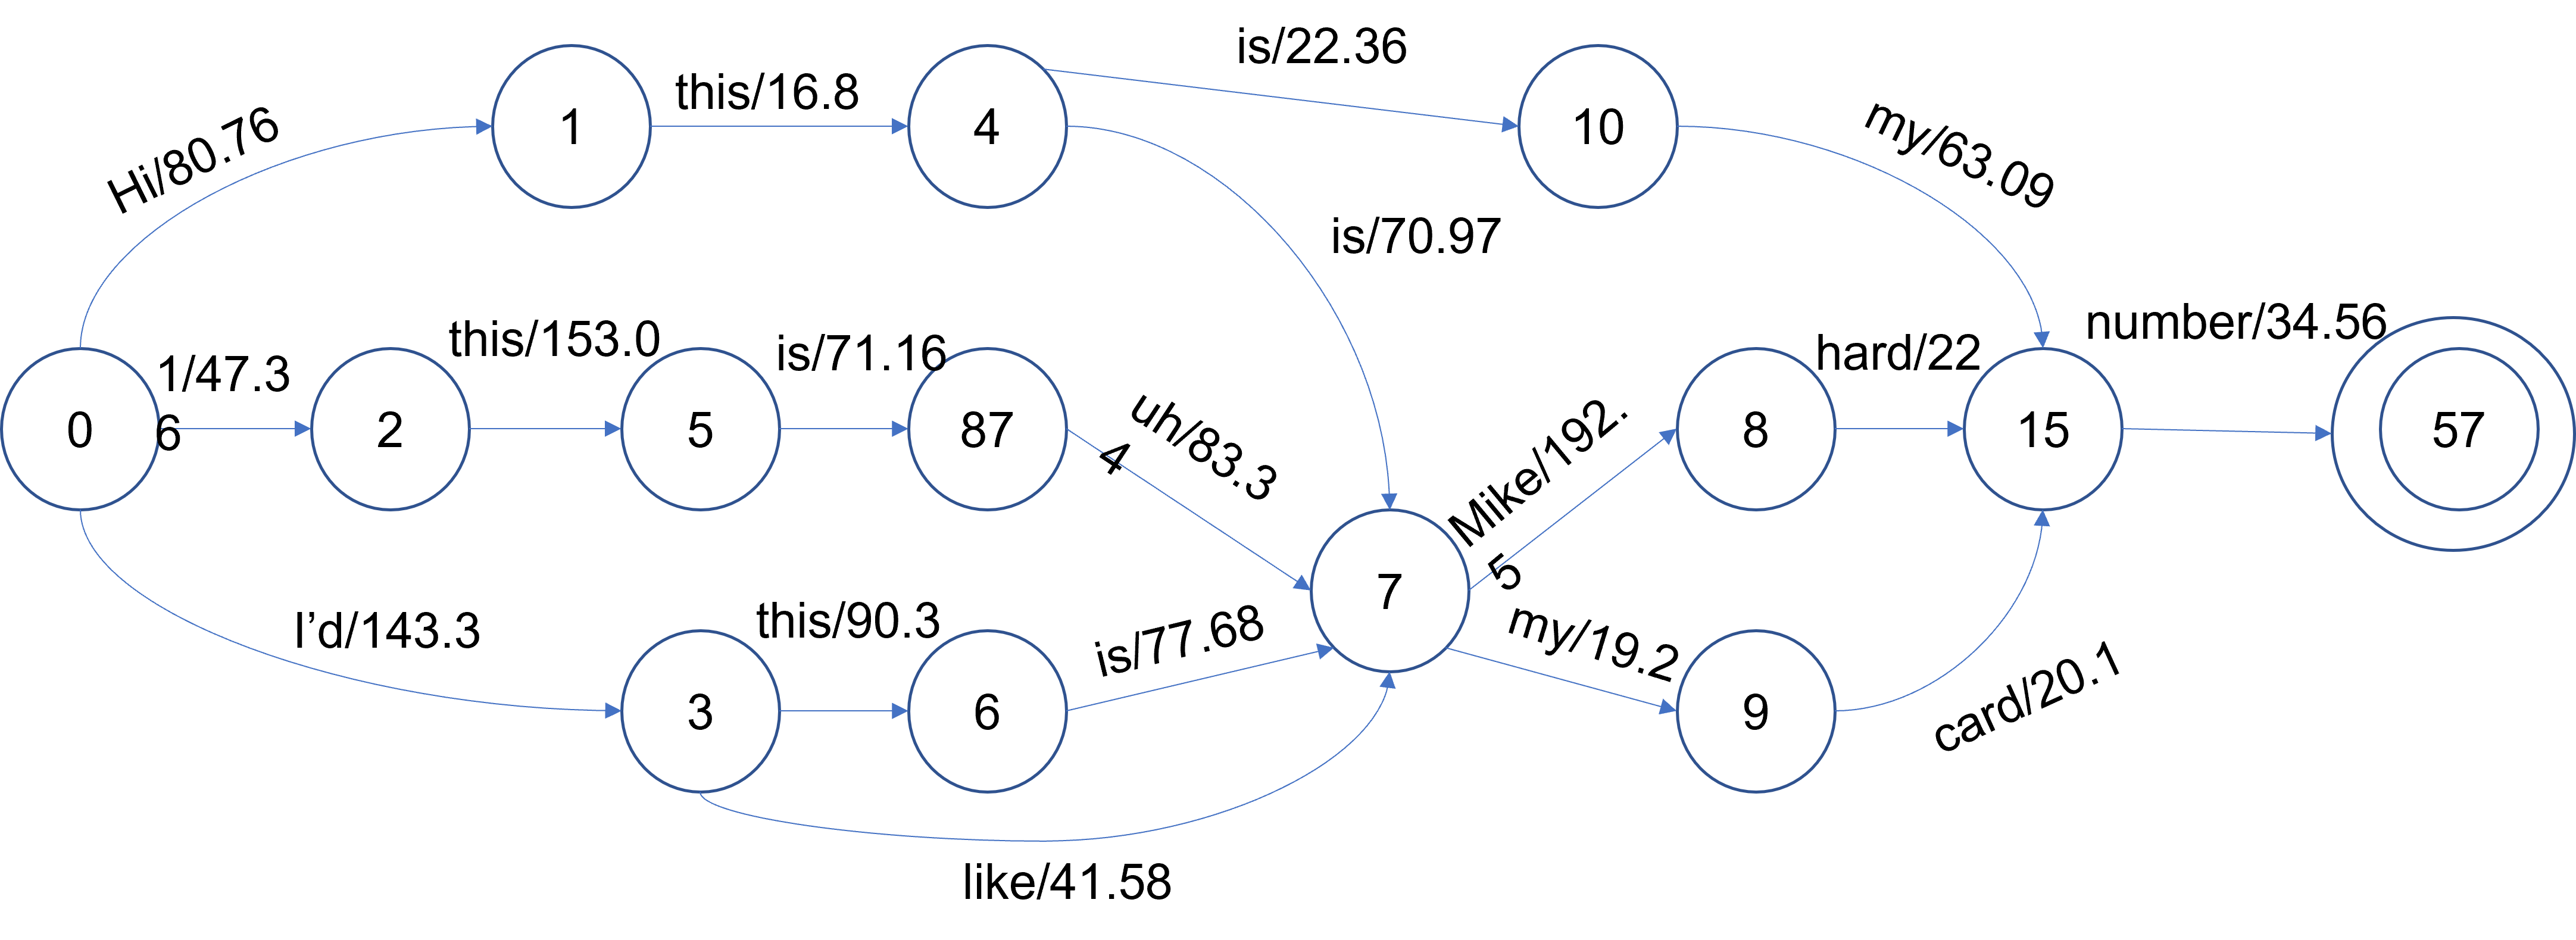
\includegraphics[width=0.9\textwidth]{img/LatticsMMI.png}
    \caption{Lattice formation}
    \label{fig:Lattice formation}
\end{figure}

Lattice-based methods were proposed prior to GPU era. It is not possible to train this deep network without a GPU but with Deep Learning in 2012 on GPUs, new possibilities emerged but the physical limitations, particularly, memory consumption problem remained. To fit the method into the GPU's memory, for example, we chop the training utterances into 1 to 1.5 second chunks which is not enough. GPU allows one GPU instruction to be run on multiple data sets one at a time. We must avoid branching to get the most benefit out of the GPU and pruned tree search does not seem so appealing with GPU which is why a smaller model is required \cite{povey_purely_2016}.

\subsection{Bypassing Lattices through Chain Model for \\ Improving Efficiency}
With the advent of E2E models, the need of a trained system for lattice initialization became a disadvantage of lattice-based MMI. Hence, comes the concept of Lattice Free MMI \cite{povey_purely_2016, ghahremani_investigation_2017} which is purely sequence trained requiring no no cross-entropy training as it does not use a lattice allowing it to exactly compute the sum instead of just approximating it \cite{noauthor_lattice_nodate}. The LF-MMI objective function is the modified form of MMI discriminative  objective function which enables ASR Training on GPU in HMM-DNN ASR Approach. 

The \textit{chain} or LFMMI models are a different form of HMM-DNN model. It uses Neural Networks \cite{daniel_povey_kaldi_nodate} which are a different point of design in the space of acoustic models compared to Traditional ASR models. It uses a three times smaller frame rate at the Neural Network output which reduces the computational requirements significantly in test-time, making decoding in real-time  much simpler. 

\begin{figure}[h]
    \centering
    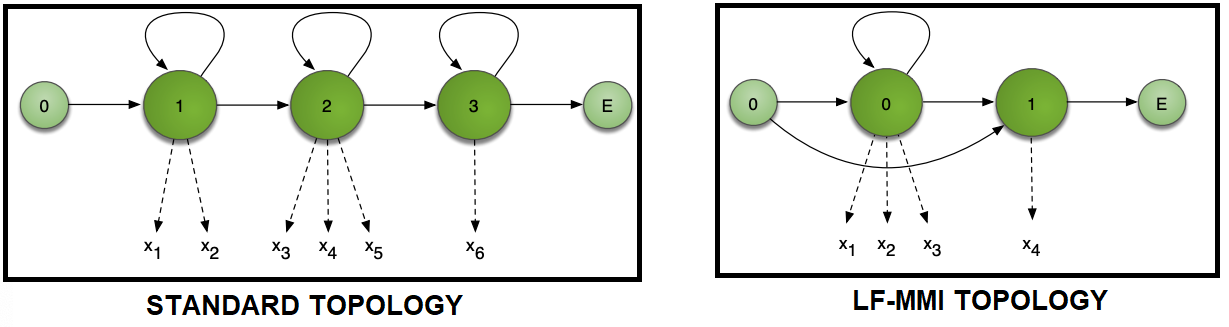
\includegraphics[width=0.8\textwidth]{img/LFMMI1.png}
    \caption{Standard vs LF-MMI Topology}
    \label{fig:LFMMI-topology}
\end{figure}

Due to the reduced frame rate, unconventional HMM topologies must be used to enable one-state HMM traversal. The chain model employs HMM's fixed transition probabilities but does not train it actually. Neural-net output probabilities can typically serve the same purpose as transition probabilities depending on the topology \cite{daniel_povey_kaldi_nodate}.

Models are trained with a sequence-level objective function, i.e. the log-probability of the correct sequence, from the start. It is implemented in an MMI-based system without lattices on GPU by performing a complete forward-backward computation on a decoding graph derived from a phone-based n-gram language model \cite{povey_purely_2016}. 

\begin{figure}[h]
    \centering
    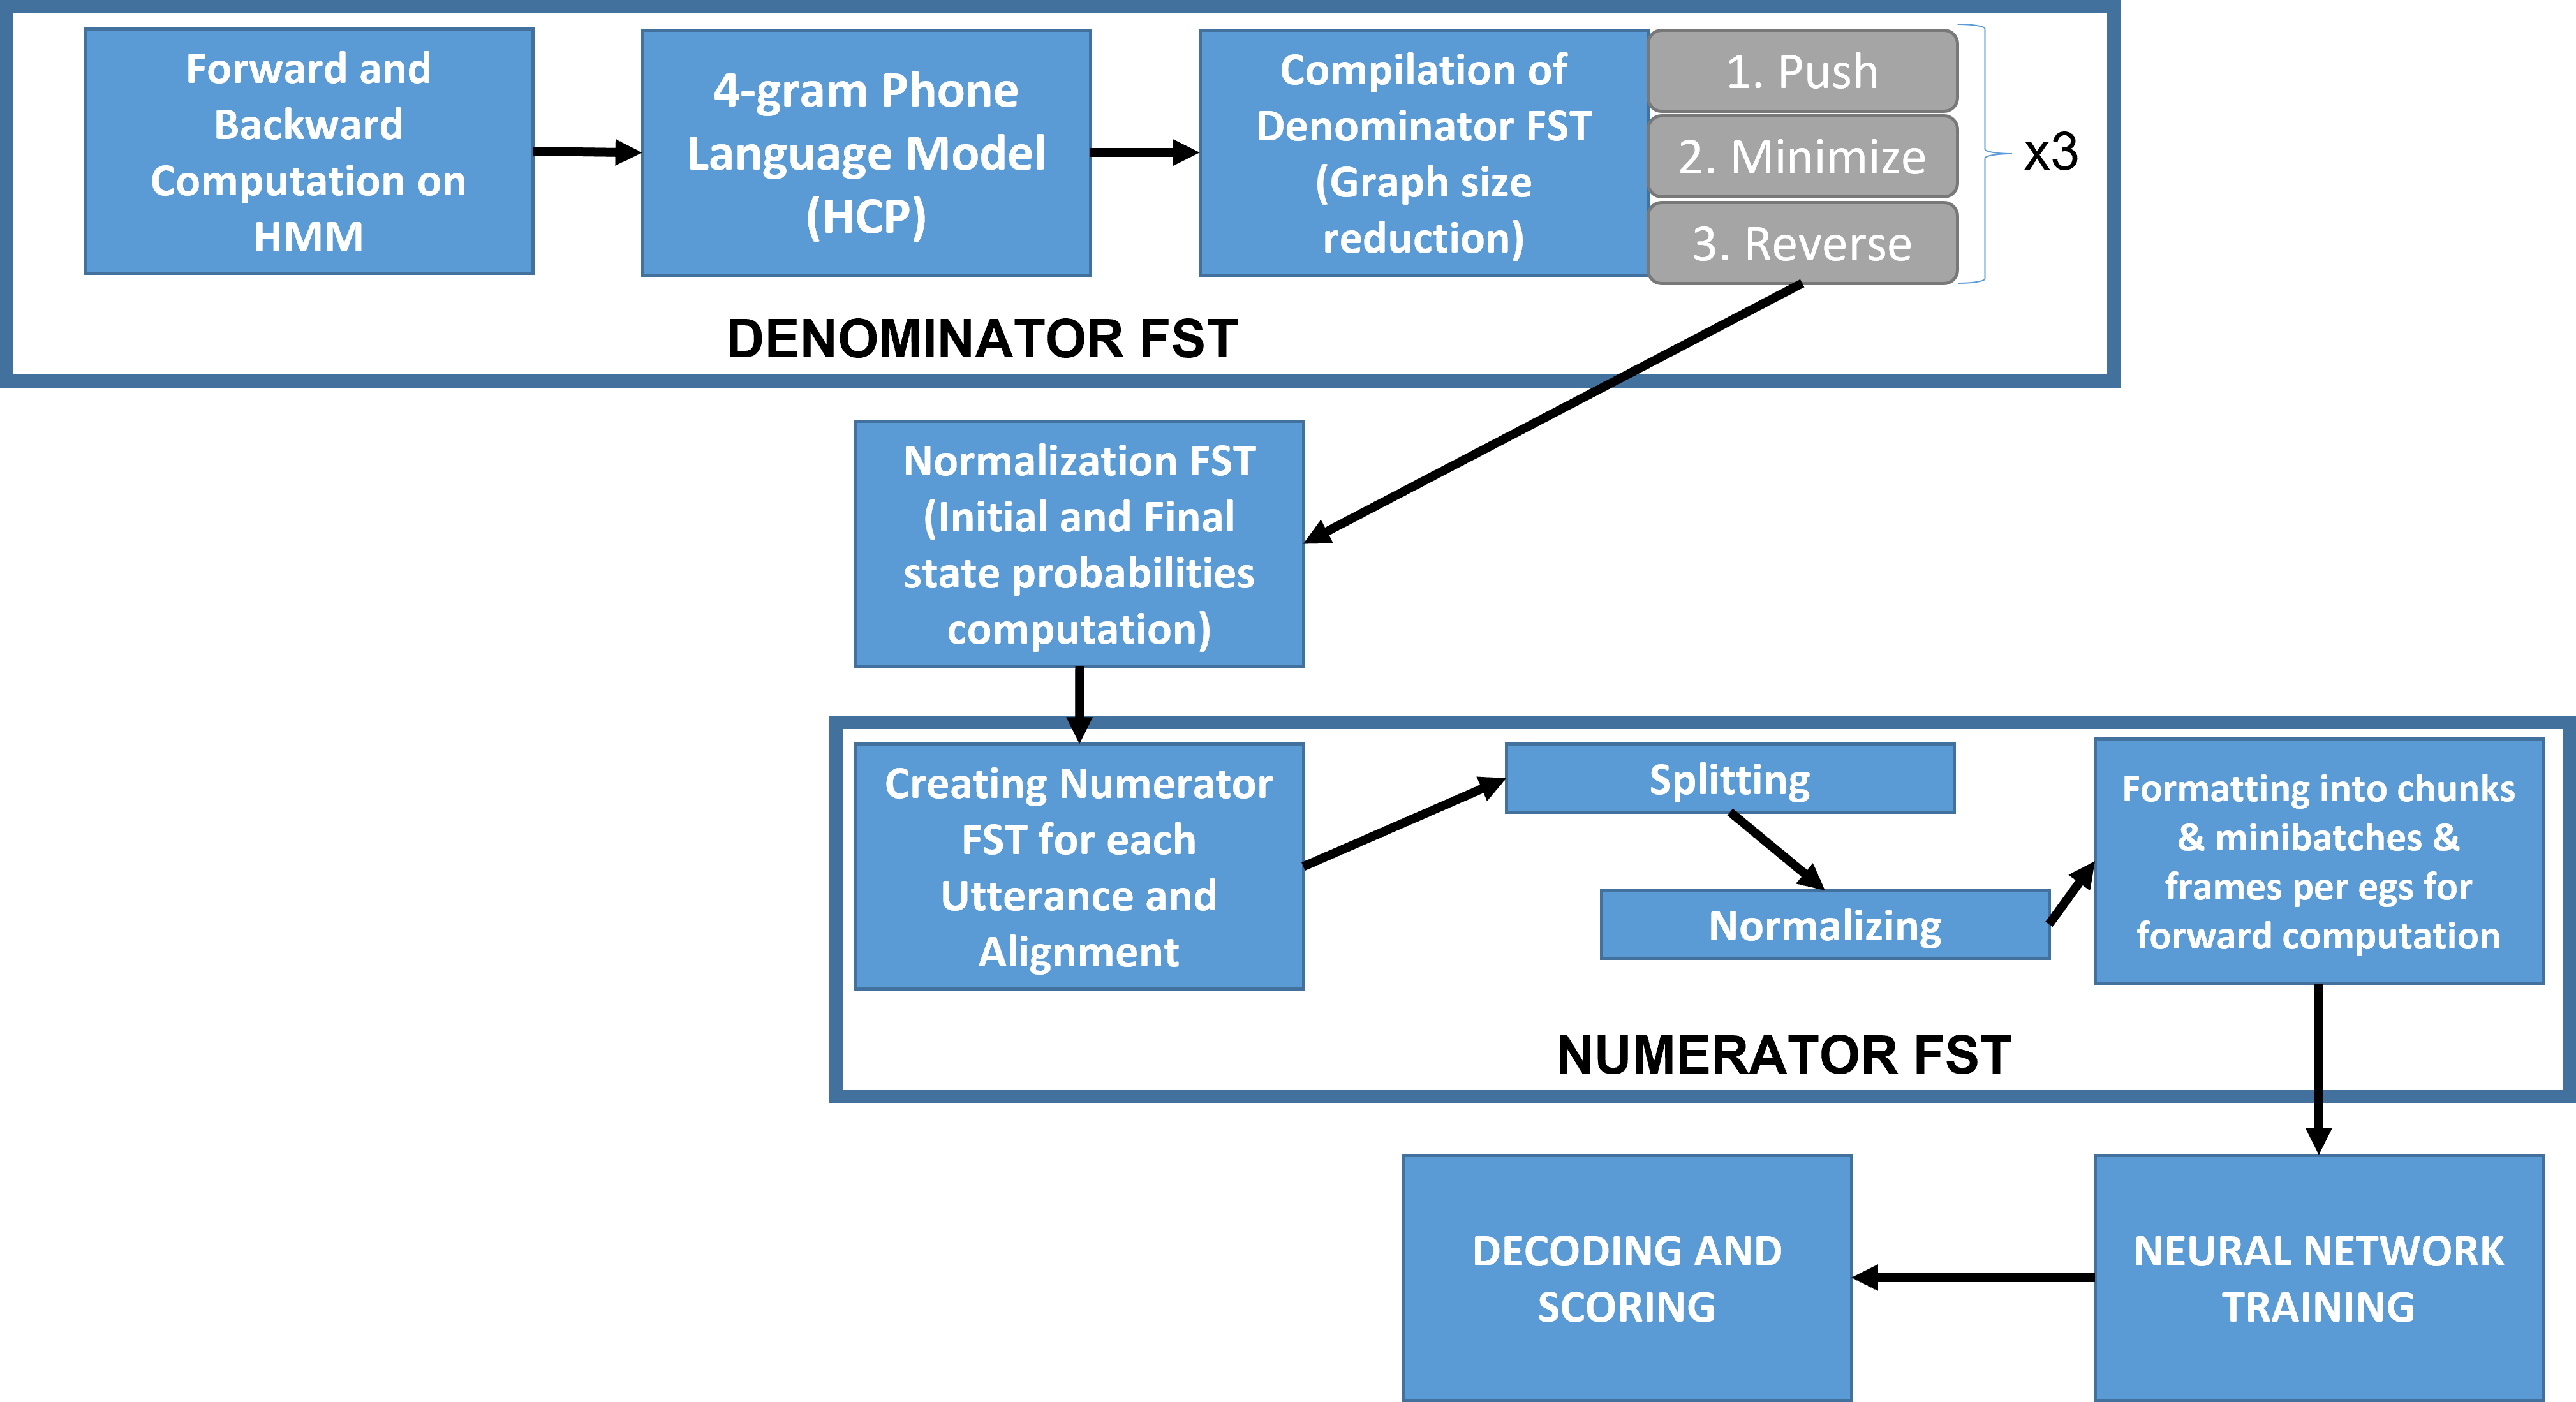
\includegraphics[width=0.9\textwidth]{img/ChainTrg.png}
    \caption{Chain Model Overview}
    \label{fig:chain-overview}
\end{figure}

%https://slideplayer.com/slide/17724439/
%https://jonathan-hui.medium.com/speech-recognition-maximum-mutual-information-estimation-mmie-a0db565764aa

If the denominator is represented as a graph and it is fitted in the GPU allowing computations to be efficiently performed for which following modifications are done \cite{noauthor_lattice_nodate, wiesner_lattice_2020}:

\begin{enumerate}
    \item Using Phone LM instead of Word-based LM to reduce size of graph significantly because there are far fewer possible phones than there are words.
    \item There are three times fewer outputs for any utterance to compute because DNN outputs are computed at a third of the standard frame-rate \cite{povey_purely_2016} which is done by decreasing the frame-shift to 30ms from traditional 10ms which means that the standard 3-state left-to-right HMM topology, commonly used in ASR, cannot be used since the entire HMM is required to be traversed in a single frame. Training such a system using the MMI objective requires the objective and its derivative to be computed effectively. 
    
\end{enumerate}

We have very limited transcribed data available for training purposes but we do have a huge amount of Call Center Data available. If we only have only a small amount of data transcribed, but much more un-transcribed data best is to train a seed model and use it to transcribe more data. But also don't want to train further on incorrect captions. So we apply data filtering based on confidence scores to select out the harder data that is most useful for refining the system. One of the solutions can be \cite{ghahremani_investigation_2017} to use a lattice to incorporate uncertainty about the transcription, and train with the LF-MMI criterion but that requires a strong language model for the best performance\cite{wallington_learning_2021}.

LF-MMI has shown to achieve better performance on various data-sets like Aspire using various different HMM-DNN and E2E ASR frameworks \cite{ghahremani_investigation_2017, tian_consistent_2022} compared to lattice based MMI model.






